% !TEX TS-program = xelatex
% Command for running this example (needs latexmkrc file):
%    latexmk -bibtex -pdf main.tex

%	نمونه پایان‌نامه آماده شده با استفاده از کلاس tehran-thesis، نگارش 1
%	سینا ممکن، دانشگاه تهران 
%	https://github.com/sinamomken/tehran-thesis
%	گروه پارسی‌لاتک
%	http://www.parsilatex.com
%	این نسخه، بر اساس نسخه‌ 0.1 از کلاس IUST-Thesis آقای محمود امین‌طوسی آماده شده است.
%        http://profsite.sttu.ac.ir/mamintoosi

%----------------------------------------------------------------------------------------------
% اگر قصد نوشتن پروژه کارشناسی را دارید، در خط زیر به جای msc، کلمه bsc و اگر قصد نوشتن رساله دکترا را دارید، کلمه phd را قرار دهید. کلیه تنظیمات لازم، به طور خودکار، اعمال می‌شود.

% اگر مایلید پایان‌نامه شما دورو باشد به جای oneside در خط زیر از twoside استفاده کنید.

% برای حاشیه‌نویسی و کم کردن صفحات ابتدایی، گزینه draft را وارد و برای نسخه نهایی آن را حذف کنید.

% برای استفاده از قلم‌های سری IR Series گزینه irfonts را وارد و برای استفاده از قلم‌های X Series 2 آن را حذف کنید.

\documentclass[
twoside
,openany
,msc
,irfonts
% ,draft
]{./tex/tehran-thesis}

% فایل commands.tex را مطالعه کنید؛ چون دستورات مربوط به فراخوانی بسته‌ها، فونت و دستورات خاص در این فایل قرار دارد.
% در این فایل، دستورها و تنظیمات مورد نیاز، آورده شده است.
%-------------------------------------------------------------------------------------------------------------------
% دستوراتی که پوشه پیش‌فرض زیرفایل‌های tex را مشخص می‌کند.
%\makeatletter
%\def\input@path{{./tex/}}
%\makeatother
% در ورژن جدید زی‌پرشین برای تایپ متن‌های ریاضی، این سه بسته، حتماً باید فراخوانی شود
\usepackage{amsthm,amssymb,amsmath}
% بسته‌ای برای تنطیم حاشیه‌های بالا، پایین، چپ و راست صفحه
\usepackage[a4paper, top=40mm, bottom=40mm, outer=25mm, inner=35mm]{geometry}
% بسته‌‌ای برای ظاهر شدن شکل‌ها و تعیین آدرس تصاویر
\usepackage[final]{graphicx}
\graphicspath{{./img/}}
% بسته‌های مورد نیاز برای نوشتن کدها، رنگ‌آمیزی آنها و تعیین پوشهٔ کدها
\usepackage[final]{listings}
\usepackage[usenames,dvipsnames,svgnames,table]{xcolor}
\lstset{inputpath=./code/}
% بسته‌ای برای رسم کادر
\usepackage{framed} 
\usepackage{tabularx}
% بسته برای هایلایت
\usepackage{soul}
% بسته‌‌ای برای چاپ شدن خودکار تعداد صفحات در صفحه «معرفی پایان‌نامه»
\usepackage{lastpage}
% بسته‌ٔ لازم برای: ۱. تغییر شماره‌گذاری صفحات پیوست. ۲. تصحیح باگ آدرس وب حاوی '%' در مراجع
\usepackage{etoolbox}

%%%%%%%%%%%%%%%%%%%%%%%%%%%%%%%%%%%%
%%% دستورات وابسته به استیل مراجع:
%% اگر از استیل‌های natbib (plainnat-fa، asa-fa، chicago-fa) استفاده می‌کنید، خط زیر را فعال و بعدی‌اش را غیرفعال کنید.
%\usepackage{natbib}
%\newcommand{\citelatin}[1]{\cite{#1}\LTRfootnote{\citeauthor*{#1}}}
%\newcommand{\citeplatin}[1]{\citep{#1}\LTRfootnote{\citeauthor*{#1}}}
%% اگر از سایر استیل‌ها استفاده می‌کنید، خط بالا را غیرفعال و خط‌های زیر را فعال کنید.
\let\citep\cite
\let\citelatin\cite
\let\citeplatin\cite
%%%%%%%%%%%%
% بررسی حالت پیش نویس
\usepackage{ifdraft}
\ifdraft
{%
	% بسته‌ٔ ایجاد لینک‌های رنگی با امکان جهش
	\usepackage[unicode=true,pagebackref=true,
colorlinks,linkcolor=blue,citecolor=blue,final]{hyperref}
	%\usepackage{todonotes}
	\usepackage[firstpage]{draftwatermark}
	\SetWatermarkText{\ \ \ \rl{پیش‌نویس}}
	\SetWatermarkScale{1.2}
}
{ 
	\usepackage[pagebackref=false]{hyperref}
	%\usepackage[disable]{todonotes} % final without TODOs
}

\usepackage[obeyDraft]{todonotes}
\setlength{\marginparwidth}{2cm}

%%%%%%%%%%%%
%%% تصحیح باگ: اگر در مراجع، آدرس وب حاوی '%' بوده و pagebackref فعال باشد، دستورات زیر باید بیایند:
%% برای استیل‌های natbib مثل plainnat-fa، asa-fa، chicago-fa
\makeatletter
\let\ORIG@BR@@lbibitem\BR@@lbibitem
\apptocmd\ORIG@BR@@lbibitem{\endgroup}{}{}
\def\BR@@lbibitem{\begingroup\catcode`\%=12 \ORIG@BR@@lbibitem}
\makeatother
%% برای سایر استیل‌ها
\makeatletter
\let\ORIG@BR@@bibitem\BR@@bibitem
\apptocmd\ORIG@BR@@bibitem{\endgroup}{}{}
\def\BR@@bibitem{\begingroup\catcode`\%=12 \ORIG@BR@@bibitem}
\makeatother
%%%%%%%%%%%%%%%%%%%%%%%%%%%%%%%%%%%%

% بسته‌ لازم برای تنظیم سربرگ‌ها
\usepackage{fancyhdr}
%\usepackage{enumitem}
\usepackage{setspace}
% بسته‌های لازم برای نوشتن الگوریتم
\usepackage{algorithm}
\usepackage{algorithmic}
% بسته‌های لازم برای رسم بهتر جداول
\usepackage{tabulary}
\usepackage{tabularx}
\usepackage{rotating}
% بسته‌های لازم برای رسم تنظیم بهتر شکل‌ها و زیرشکل‌ها
\usepackage[export]{adjustbox}
\usepackage{subfig}
\usepackage[subfigure]{tocloft}
% بسته‌ای برای رسم نمودارها و نیز صفحه مالکیت اثر
\usepackage{tikz}
% رسم بهتر جدول
\usepackage{booktabs} % برای خطوط نازک تر
\usepackage{makecell} % برای تنظیم متن داخل سلول ها
% بسته‌ای برای ظاهر شدن «مراجع» و «نمایه» در فهرست مطالب
\usepackage[nottoc]{tocbibind}
% دستورات مربوط به ایجاد نمایه
\usepackage{makeidx}
\makeindex
%%% بسته ایجاد واژه‌نامه با xindy
\usepackage[xindy,toc,acronym,nonumberlist=true]{glossaries}

% بسته‌ای برای افزودن تورفتگی به ابتدای اولین پاراگراف هر بخش
\usepackage{indentfirst}

% بسته زیر باگ ناشی از فراخوانی بسته‌های زیاد را برطرف می‌کند.
\usepackage{morewrites}
%%%%%%%%%%%%%%%%%%%%%%%%%%
\usepackage{fontspec}
\usepackage{bidi}

% فراخوانی بسته زی‌پرشین (باید آخرین بسته باشد)
\usepackage[extrafootnotefeatures, localise=on, displaymathdigits=persian,perpagefootnote=on]{xepersian}




\makeatletter
% تعریف قلم فارسی و انگلیسی و مکان قلم‌ها
\if@irfonts
\settextfont[Path={./font/}, BoldFont={IRLotusICEE_Bold.ttf}, BoldItalicFont={IRLotusICEE_BoldIranic.ttf}, ItalicFont={IRLotusICEE_Iranic.ttf},Scale=1.2]{IRLotusICEE.ttf}
% LiberationSerif or FreeSerif as free equivalents of Times New Roman
\setlatintextfont[Path={./font/}, BoldFont={LiberationSerif-Bold.ttf}, BoldItalicFont={LiberationSerif-BoldItalic.ttf}, ItalicFont={LiberationSerif-Italic.ttf},Scale=1]{LiberationSerif-Regular.ttf}
% چنانچه می‌خواهید اعداد در فرمول‌ها، انگلیسی باشد، خط زیر را غیرفعال کنید
% و گزینهٔ displaymathdigits=persian را از خط ۱۰۹ حذف کنید.
\setdigitfont[Path={./font/}, Scale=1.2]{IRLotusICEE.ttf}
% تعریف قلم‌های فارسی و انگلیسی اضافی برای استفاده در بعضی از قسمت‌های متن
\setiranicfont[Path={./font/}, Scale=1.3]{IRLotusICEE_Iranic.ttf}				% ایرانیک، خوابیده به چپ
\setmathsfdigitfont[Path={./font/}]{IRTitr.ttf}
\defpersianfont\titlefont[Path={./font/}, Scale=1]{IRTitr.ttf}
% برای تعریف یک قلم خاص عنوان لاتین، خط بعد را فعال و ویرایش کنید و خط بعد از آن را غیرفعال کنید.
% \deflatinfont\latintitlefont[Scale=1]{LiberationSerif}
\font\latintitlefont=cmssbx10 scaled 2300 %cmssbx10 scaled 2300
\else
\settextfont{XB Niloofar}
\setlatintextfont{Junicode}
% چنانچه می‌خواهید اعداد در فرمول‌ها، انگلیسی باشد، خط زیر را غیرفعال کنید
% و گزینهٔ displaymathdigits=persian را از خط ۱۰۹ حذف کنید.
\setdigitfont{XB Niloofar}
% تعریف قلم‌های فارسی و انگلیسی اضافی برای استفاده در بعضی از قسمت‌های متن
% \setmathsfdigitfont{XB Titre}
\defpersianfont\titlefont{XB Titre}
\deflatinfont\latintitlefont[Scale=1.1]{Junicode}
\fi
\makeatother

% برای استفاده از قلم نستعلیق خط بعد را فعال کنید.
% \defpersianfont\nastaliq[Scale=1.2]{IranNastaliq}


%%%%%%%%%%%%%%%%%%%%%%%%%%
% راستچین شدن todonotes
\presetkeys{todonotes}{align=right,textdirection=righttoleft}{}
\makeatletter
\providecommand\@dotsep{5}
\def\listtodoname{فهرست کارهای باقیمانده}
\def\listoftodos{\noindent{\Large\vspace{10mm}\textbf{\listtodoname}}\@starttoc{tdo}}
\renewcommand{\@todonotes@MissingFigureText}{شکل}
\renewcommand{\@todonotes@MissingFigureUp}{شکل}
\renewcommand{\@todonotes@MissingFigureDown}{جاافتاده}
\makeatother
%کد رسم جدول
\newcommand\mrh{\color{white}\bfseries}
\newcommand\mrc[1]{\begin{tabular}{@{}l@{}} #1 \end{tabular}}
\setlength\arrayrulewidth{0.8pt}
% دستوری برای حذف کلمه «چکیده»
% \renewcommand{\abstractname}{}
% دستوری برای حذف کلمه «abstract»
%\renewcommand{\latinabstract}{}
% دستوری برای تغییر نام کلمه «اثبات» به «برهان»
\renewcommand\proofname{\textbf{برهان}}
% دستوری برای تغییر نام کلمه «کتاب‌نامه» به «مراجع»
\renewcommand{\bibname}{مراجع}
% دستوری برای تعریف واژه‌نامه انگلیسی به فارسی
\newcommand\persiangloss[2]{#1\dotfill\lr{#2}\\}
% دستوری برای تعریف واژه‌نامه فارسی به انگلیسی 
\newcommand\englishgloss[2]{#2\dotfill\lr{#1}\\}
% تعریف دستور جدید «\پ» برای خلاصه‌نویسی جهت نوشتن عبارت «پروژه/پایان‌نامه/رساله»
\newcommand{\پ}{پروژه/پایان‌نامه/رساله }

%\newcommand\BackSlash{\char`\\}

%%%%%%%%%%%%%%%%%%%%%%%%%%
% \SepMark{-}

% تعریف و نحوه ظاهر شدن عنوان قضیه‌ها، تعریف‌ها، مثال‌ها و ...
\theoremstyle{definition}
\newtheorem{definition}{تعریف}[section]
\theoremstyle{theorem}
\newtheorem{theorem}[definition]{قضیه}
\newtheorem{lemma}[definition]{لم}
\newtheorem{proposition}[definition]{گزاره}
\newtheorem{corollary}[definition]{نتیجه}
\newtheorem{remark}[definition]{ملاحظه}
\theoremstyle{definition}
\newtheorem{example}[definition]{مثال}

%\renewcommand{\theequation}{\thechapter-\arabic{equation}}
%\def\bibname{مراجع}
\numberwithin{algorithm}{chapter}
%\def\listalgorithmname{فهرست الگوریتم‌ها}
\def\listfigurename{فهرست تصاویر}
%\def\listtablename{فهرست جداول}

% دستور های لازم برای تعریف ترجمهٔ دستورات الگوریتم
\makeatletter
\renewcommand{\algorithmicrequire}{\if@RTL\textbf{ورودی:}\else\textbf{Require:}\fi}
\renewcommand{\algorithmicensure}{\if@RTL\textbf{خروجی:}\else\textbf{Ensure:}\fi}
\renewcommand{\algorithmicend}{\if@RTL\textbf{پایان}\else\textbf{end}\fi}
\renewcommand{\algorithmicif}{\if@RTL\textbf{اگر}\else\textbf{if}\fi}
\renewcommand{\algorithmicthen}{\if@RTL\textbf{آنگاه}\else\textbf{then}\fi}
\renewcommand{\algorithmicelse}{\if@RTL\textbf{وگرنه}\else\textbf{else}\fi}
\renewcommand{\algorithmicfor}{\if@RTL\textbf{برای}\else\textbf{for}\fi}
\renewcommand{\algorithmicforall}{\if@RTL\textbf{برای هر}\else\textbf{for all}\fi}
\renewcommand{\algorithmicdo}{\if@RTL\textbf{انجام بده}\else\textbf{do}\fi}
\renewcommand{\algorithmicwhile}{\if@RTL\textbf{تا زمانی که}\else\textbf{while}\fi}
\renewcommand{\algorithmicloop}{\if@RTL\textbf{تکرار کن}\else\textbf{loop}\fi}
\renewcommand{\algorithmicrepeat}{\if@RTL\textbf{تکرار کن}\else\textbf{repeat}\fi}
\renewcommand{\algorithmicuntil}{\if@RTL\textbf{تا زمانی که}\else\textbf{until}\fi}
\renewcommand{\algorithmicprint}{\if@RTL\textbf{چاپ کن}\else\textbf{print}\fi}
\renewcommand{\algorithmicreturn}{\if@RTL\textbf{بازگردان}\else\textbf{return}\fi}
\renewcommand{\algorithmicand}{\if@RTL\textbf{و}\else\textbf{and}\fi}
\renewcommand{\algorithmicor}{\if@RTL\textbf{و یا}\else\textbf{or}\fi} % TODO add better translate
\renewcommand{\algorithmicxor}{\if@RTL\textbf{یا}\else\textbf{xor}\fi} % TODO add better translate
\renewcommand{\algorithmicnot}{\if@RTL\textbf{نقیض}\else\textbf{not}\fi}
\renewcommand{\algorithmicto}{\if@RTL\textbf{تا}\else\textbf{to}\fi}
\renewcommand{\algorithmicinputs}{\if@RTL\textbf{ورودی‌ها}\else\textbf{inputs}\fi}
\renewcommand{\algorithmicoutputs}{\if@RTL\textbf{خروجی‌ها}\else\textbf{outputs}\fi}
\renewcommand{\algorithmicglobals}{\if@RTL\textbf{متغیرهای عمومی}\else\textbf{globals}\fi}
\renewcommand{\algorithmicbody}{\if@RTL\textbf{انجام بده}\else\textbf{do}\fi}
\renewcommand{\algorithmictrue}{\if@RTL\textbf{درست}\else\textbf{true}\fi}
\renewcommand{\algorithmicfalse}{\if@RTL\textbf{نادرست}\else\textbf{false}\fi}
\renewcommand{\algorithmicendif}{\algorithmicend\textbf{ شرط }\algorithmicif}
\renewcommand{\algorithmicendfor}{\algorithmicend\textbf{ حلقهٔ }\algorithmicfor}
\renewcommand{\algorithmicendwhile}{\algorithmicend\textbf{ حلقهٔ }\algorithmicwhile}
\renewcommand{\algorithmicendloop}{\algorithmicend\textbf{ حلقهٔ }\algorithmicloop}
\renewcommand{\algorithmiccomment}[1]{\{{\itshape #1}\}}
\makeatletter

%%%%%%%%%%%%%%%%%%%%%%%%%%%%
%%% دستورهایی برای سفارشی کردن سربرگ صفحات:
%\newcommand{\SetHeader}[1]{
% دستور زیر معادل با گزینه twoside است.
%\csname@twosidetrue\endcsname
\pagestyle{fancy}
%% دستورات زیر سبک صفحات fancy را تغییر می‌دهد:
% O=Odd, E=Even, L=Left, R=Right
% در صورت oneside بودن، عنوان فصل، سمت چپ ظاهر می‌شود.
\fancyhead{}
\fancyhead[OL]{\small\leftmark}
\fancyhead[ER]{\small\leftmark}
\fancyhead[OR]{\footnotesize\rightmark}
\fancyhead[EL]{\footnotesize\rightmark}
\renewcommand{\headrulewidth}{0.75pt}
% شکل‌دهی شماره و عنوان فصل در سربرگ
\renewcommand{\chaptermark}[1]{\markboth{\@chapapp~\thechapter:\ #1}{}}
\makeatletter
\renewcommand{\rightmark}[1]{\@title}
\makeatother
%}
%%%%%%%%%%%%%%%%%%%%%%%%%%%%
%\def\MATtextbaseline{1.5}
%\renewcommand{\baselinestretch}{\MATtextbaseline}
\doublespacing
%%%%%%%%%%%%%%%%%%%%%%%%%%%%%
% دستوراتی برای اضافه کردن کلمه «فصل» در فهرست مطالب

\newlength\mylenprt
\newlength\mylenchp
\newlength\mylenapp

\renewcommand\cftpartpresnum{\partname~}
\renewcommand\cftchappresnum{\chaptername~}
\renewcommand\cftchapaftersnum{:}

\settowidth\mylenprt{\cftpartfont\cftpartpresnum\cftpartaftersnum}
\settowidth\mylenchp{\cftchapfont\cftchappresnum\cftchapaftersnum}
\settowidth\mylenapp{\cftchapfont\appendixname~\cftchapaftersnum}
\addtolength\mylenprt{\cftpartnumwidth}
\addtolength\mylenchp{\cftchapnumwidth}
\addtolength\mylenapp{\cftchapnumwidth}

\setlength\cftpartnumwidth{\mylenprt}
\setlength\cftchapnumwidth{\mylenchp}	

\makeatletter
{\def\thebibliography#1{\chapter*{\refname\@mkboth
   {\uppercase{\refname}}{\uppercase{\refname}}}\list
   {[\arabic{enumi}]}{\settowidth\labelwidth{[#1]}
   \rightmargin\labelwidth
   \advance\rightmargin\labelsep
   \advance\rightmargin\bibindent
   \itemindent -\bibindent

   \listparindent \itemindent
   \parsep \z@
   \usecounter{enumi}}
   \def\newblock{}
   \sloppy
   \sfcode`\.=1000\relax}}
   
%اگر مایلید در شماره گذاری حرفی و ابجد به جای آ از الف استفاده شود دستورات زیر را فعال کنید.   
%\def\@Abjad#1{%
%  \ifcase#1\or الف\or ب\or ج\or د%
%           \or هـ\or و\or ز\or ح\or ط%
%           \or ی\or ک\or ل\or م\or ن%
%           \or س\or ع\or ف\or ص%
%           \or ق\or ر\or ش\or ت\or ث%
%            \or خ\or ذ\or ض\or ظ\or غ%
%            \else\@ctrerr\fi}
%
% \def\abj@num@i#1{%
%   \ifcase#1\or الف\or ب\or ج\or د%
%            \or هـ‍\or و\or ز\or ح\or ط\fi

%   \ifnum#1=\z@\abjad@zero\fi}   
%  
%   \def\@harfi#1{\ifcase#1\or الف\or ب\or پ\or ت\or ث\or

% ج\or چ\or ح\or خ\or د\or ذ\or ر\or ز\or ژ\or س\or ش\or ص\or ض\or ط\or ظ\or ع\or غ\or

% ف\or ق\or ک\or گ\or ل\or م\or ن\or و\or ه\or ی\else\@ctrerr\fi}

%
\makeatother

%%% امکان درج کد در سند
% در این قسمت رنگ، قلم و قالب‌بندی قسمت‌های مختلف یک کد تعیین می‌شود. 
\lstdefinestyle{myStyle}{
	basicstyle=\ttfamily, % whole listing /w verbatim font
	keywordstyle=\color{blue}\bfseries, % bold black keywords
	identifierstyle=, % nothing happens
	commentstyle=\color{LimeGreen}, % green comments
	stringstyle=\ttfamily\color{red}, % red typewriter font for strings
	showstringspaces=false % no special string spaces
	breaklines=true,
	breakatwhitespace=false,
	numbers=right, % line number formats
	numberstyle=\footnotesize\lr,
	numbersep=-10pt,
	frame=single,
	captionpos=b,
	captiondirection=RTL
}
\lstset{style=myStyle} % command to set default style
\def\lstlistingname{\rl{برنامهٔ}}
\def\lstlistlistingname{\rl{فهرست برنامه‌ها}}


% for numbering subsubsections
\setcounter{secnumdepth}{3}
%to include subsubsections in the table of contents
\setcounter{tocdepth}{3}


\makeatletter
\renewcommand{\p@subfigure}{\thefigure.}
\makeatother

% مشخصات پایان‌نامه را در فایلهای faTitle و enTitle وارد نمایید.
% !TeX root=../main.tex
% در این فایل، عنوان پایان‌نامه، مشخصات خود، متن تقدیمی‌، ستایش، سپاس‌گزاری و چکیده پایان‌نامه را به فارسی، وارد کنید.
% توجه داشته باشید که جدول حاوی مشخصات پروژه/پایان‌نامه/رساله و همچنین، مشخصات داخل آن، به طور خودکار، درج می‌شود.
%%%%%%%%%%%%%%%%%%%%%%%%%%%%%%%%%%%%
% دانشگاه خود را وارد کنید
\university{دانشگاه تبریز}
% دانشکده، آموزشکده و یا پژوهشکده  خود را وارد کنید
\faculty{دانشکدهٔ مهندسی برق و کامپیوتر}
% گروه آموزشی خود را وارد کنید (در صورت نیاز)
\department{گروه مهندسی کامپیوتر}
% رشته تحصیلی خود را وارد کنید
\subject{مهندسی کامپیوتر}
% گرایش خود را وارد کنید
\field{معماری سیستم های کامپیوتری}
% عنوان پایان‌نامه را وارد کنید
\title{شبکه ارتباط سنج انسان-اشیاء و انسان-ژست برای تشخیص فعالیت انسان در تک تصویر }
% نام استاد(ان) راهنما را وارد کنید
\firstsupervisor{دکتر عبدالحمید معلمی خیاوی}
\firstsupervisorrank{استادیار}
%\secondsupervisor{دکتر راهنمای دوم}
%\secondsupervisorrank{استادیار}
% نام استاد(دان) مشاور را وارد کنید. چنانچه استاد مشاور ندارید، دستورات پایین را غیرفعال کنید.
\firstadvisor{دکتر علیرضا سخندان سرخابی}
\firstadvisorrank{استادیار}
%\secondadvisor{دکتر مشاور دوم}
% نام داوران داخلی و خارجی خود را وارد نمایید.
\internaljudge{دکتر داور داخلی}
\internaljudgerank{دانشیار}
\externaljudge{دکتر داور خارجی}
\externaljudgerank{دانشیار}
\externaljudgeuniversity{دانشگاه داور خارجی}
% نام نماینده کمیته تحصیلات تکمیلی در دانشکده \ گروه
\graduatedeputy{دکتر نماینده}
\graduatedeputyrank{دانشیار}
% نام دانشجو را وارد کنید
\name{مهران}
% نام خانوادگی دانشجو را وارد کنید
\surname{شاه محمدی}
% شماره دانشجویی دانشجو را وارد کنید
\studentID{999482103}
% تاریخ پایان‌نامه را وارد کنید
\thesisdate{بهمن 1402}
% به صورت پیش‌فرض برای پایان‌نامه‌های کارشناسی تا دکترا به ترتیب از عبارات «پروژه»، «پایان‌نامه» و «رساله» استفاده می‌شود؛ اگر  نمی‌پسندید هر عنوانی را که مایلید در دستور زیر قرار داده و آنرا از حالت توضیح خارج کنید.
%\projectLabel{پایان‌نامه}

% به صورت پیش‌فرض برای عناوین مقاطع تحصیلی کارشناسی تا دکترا به ترتیب از عبارت «کارشناسی»، «کارشناسی ارشد» و «دکتری» استفاده می‌شود؛ اگر نمی‌پسندید هر عنوانی را که مایلید در دستور زیر قرار داده و آنرا از حالت توضیح خارج کنید.
%\degree{}
%%%%%%%%%%%%%%%%%%%%%%%%%%%%%%%%%%%%%%%%%%%%%%%%%%%%
%% پایان‌نامه خود را تقدیم کنید! %%
\dedication
{
{\Large تقدیم به:}\\
\begin{flushleft}{
	\huge
	پدر و مادرم
}
\end{flushleft}
}
%% متن قدردانی %%
%% ترجیحا با توجه به ذوق و سلیقه خود متن قدردانی را تغییر دهید.
\acknowledgement{
سپاس خداوندگار حکیم را که با لطف بی‌کران خود، آدمی را به زیور عقل آراست.

در آغاز وظیفه‌  خود  می‌دانم از زحمات بی‌دریغ اساتید  راهنمای خود،  جناب آقای دکتر \textbf{عبدالحمید معلمی خیاوی} صمیمانه تشکر و  قدردانی کنم که در طول انجام این پایان‌نامه با نهایت صبوری همواره راهنما و مشوق من بودند و قطعاً بدون راهنمایی‌های ارزنده‌ ایشان، این مجموعه به انجام نمی‌رسید.

از جناب آقای دکتر \textbf{علیرضا سخندان} که  زحمت مشاوره‌، بازبینی و تصحیح این پایان‌نامه را تقبل فرمودند کمال امتنان را دارم.

و در پایان، بوسه می‌زنم بر دستان خداوندگاران مهر و مهربانی، پدر و مادر عزیزم و بعد از خدا، ستایش می‌کنم وجود مقدس‌شان را و تشکر می‌کنم از خانواده عزیزم به پاس عاطفه سرشار و گرمای امیدبخش وجودشان، که بهترین پشتیبان من بودند.
}
%%%%%%%%%%%%%%%%%%%%%%%%%%%%%%%%%%%%
%چکیده پایان‌نامه را وارد کنید
\fa-abstract{
به دلیل عدم وجود اطلاعات زمانی در تک تصویر، استفاده از روشهای متداول پردازش ویدیو برای شناسایی و تشخیص نوع فعالیت انسانی امکان پذیر نمی‌باشد و در نتیجه تشخیص این اطلاعات در تک تصویر با چالش‌های فراوانی روبرو است. برای جبران عدم وجود اطلاعات زمانی، تمرکز روی اطلاعات جانبی تصویر و پس‌زمینه کارآمد است. از تک تصویر می‌توان اطلاعاتی ازجمله شکل ظاهری انسان، ژست و اشیاء مرتبط با انسان را استخراج کرد. شکل ظاهری انسان، ژست و اشیاء مرتبط با انسان شامل اطلاعات مهمی از فعالیت انسان است، امروزه جهت استخراج این ویژگی‌ها از شبکه های عصبی عمیق  استفاده می‌شود. همچنین شبکه ترنسفرمر و مکانیزم توجه که نخست درکاربرد پردازش متن استفاده می‌شد ولی امروزه در زمینه بینایی کامپیوتر نیز بسیار مورد استفاده قرارمی‌گیرد. تشخیص فعالیت انسان در تک تصویر کاربردهای متنوعی دارد ازجمله نظارت، صنعت رباتیک، برنامه‌های تعامل انسان و کامپیوتر، برچسب گذاری فریم ها و غیره. دراین پایان نامه با استفاده از شبکه‌های عصبی عمیق، ابتدا ویژگی‌های مهم تصویر استخراج می‌شود، سپس این ویژگی‌ها با کمک مکانیزم توجه با یکدیگر ترکیب شده تا یک ارتباط‌سنجی انجام شود و رابطه بین انسان و ژست، و همچنین رابطه انسان و اشیاء مرتبط مشخص شود و شبکه نسبت به این نتایج ارتباط‌سنجی شده، فعالیت را تخمین بزند. برای ترکیب ژست با انسان از توصیف کننده زاویه بدن جهت استخراج ویژگی ژست استفاده شده است. دو مجموعه داده %
\lr{VOC‌ 2012}
 و 
\lr{Stanford40}
 در زمینه فعالیت انسان برای ارزیابی کارایی مدل و آموزش شبکه مورد استفاده قرار می‌گیرد. نتیجه مدل  پیشنهادی توصیف کننده زاویه بدن در ترکیب با خروجی بخش ارتباط‌سنج روی مجموعه داده %
\lr{VOC‌ 2012}
 دقت %
 \lr{92.33\%}
را بدست آورده است.
}
% کلمات کلیدی پایان‌نامه را وارد کنید
\keywords{تشخیص فعالیت انسان در تک تصویر، یادگیری عمیق، مکانیزم توجه، تخمین ژست، شناسایی اشیاء}
% انتهای وارد کردن فیلد‌ها
%%%%%%%%%%%%%%%%%%%%%%%%%%%%%%%%%%%%%%%%%%%%%%%%%%%%%%

% مشخصات انگلیسی پایان‌نامه
% !TeX root=../main.tex
% در این فایل، عنوان پایان‌نامه، مشخصات خود و چکیده پایان‌نامه را به انگلیسی، وارد کنید.

%%%%%%%%%%%%%%%%%%%%%%%%%%%%%%%%%%%%
\latinuniversity{University of Tabriz}
\latinfaculty{Faculty of Electrical and Computer Engineering}
\latindepartment{Computer Engineering Group}
\latinsubject{Computer Engineering}
\latinfield{Computer Systems Architecture}
\latintitle{Human-Object and Human-Pose relation network for human action recognition in still images}
\firstlatinsupervisor{Dr. Abdolhamid Moallemi Khiavi}
%\secondlatinsupervisor{Dr. Alireza Sokhandan Sorkhabi}
\firstlatinadvisor{Dr. Alireza Sokhandan Sorkhabi}
%\secondlatinadvisor{Second Advisor}
\latinname{Mehran}
\latinsurname{Shahmohammadi}
\latinthesisdate{May 2023}
\latinkeywords{
Human Action Recognition in Still Image, Deep Learning, Attention Mechanism, Pose Estimation, Object Detection}
\en-abstract{
The identification and recognition of human activities from a single image pose significant challenges due to the absence of temporal information. Conventional video processing methods are ineffective in this context. To address these challenges, we propose a novel image-based Human Action Recognition (HAR) method that utilizes both Deep Neural Networks (DNNs) and Transformers. Our method effectively compensates for the lack of temporal information by focusing on the image's auxiliary and contextual information.
From a single image, information such as human appearance, pose and objects related to humans can be extracted. These pieces of information encompass crucial details of human actions and deep neural networks are commonly employed today to extract these features.
The Transformer network and Attention Mechanism, initially used in text processing, are now widely utilized in computer vision as well. Recognizing human action in a still image has various applications including surveillance, robotics industry, human-computer interaction programs, frame tagging, and more. In this thesis, important image features are first extracted using deep neural networks. Then, these features are combined with each other using the attention mechanism to perform relational reasoning. The relationship between human and pose, as well as the relationship between human and relevant objects, is identified. The network estimates action based on these relational results. To combine pose with human, limb angle descriptors are used to extract pose features. The VOC 2012 and Stanford40 datasets in the field of human action are used to evaluate the model's performance and train the network. The proposed model's result, combining limb angle descriptors with the output of the relational reasoning component, achieves an accuracy of 92.33\% on the VOC 2012 dataset.
}


% تنظیمات و تعاریف واژه‌نامه و اختصارات
%%% تنظیمات مربوط به بسته  glossaries
%%% تعریف استایل برای واژه‌نامه فارسی به انگلیسی، در این استایل واژه‌های فارسی در سمت راست و واژه‌های انگلیسی در سمت چپ خواهند آمد. از حالت گروه ‌بندی استفاده می‌کنیم، 
%%% یعنی واژه‌ها در گروه‌هایی به ترتیب حروف الفبا مرتب می‌شوند، مثلا:
%%% الف
%%% افتصاد ................................... Economy
%%% اشکال ........................................ Failure
%%% ش
%%% شبکه ...................................... Network
\newglossarystyle{myFaToEn}{%
	\renewenvironment{theglossary}{}{}
	\renewcommand*{\glsgroupskip}{\vskip 10mm}
	\renewcommand*{\glsgroupheading}[1]{\subsection*{\glsgetgrouptitle{##1}}}
	\renewcommand*{\glossentry}[2]{\noindent\glsentryname{##1}\dotfill\space \glsentrytext{##1}
		
	}
}

%% % تعریف استایل برای واژه‌نامه انگلیسی به فارسی، در این استایل واژه‌های فارسی در سمت راست و واژه‌های انگلیسی در سمت چپ خواهند آمد. از حالت گروه ‌بندی استفاده می‌کنیم، 
%% % یعنی واژه‌ها در گروه‌هایی به ترتیب حروف الفبا مرتب می‌شوند، مثلا:
%% % E
%%% Economy ............................... اقتصاد
%% % F
%% % Failure................................... اشکال
%% %N
%% % Network ................................. شبکه

\newglossarystyle{myEntoFa}{%
	%%% این دستور در حقیقت عملیات گروه‌بندی را انجام می‌دهد. بدین صورت که واژه‌ها در بخش‌های جداگانه گروه‌بندی می‌شوند، 
	%%% عنوان بخش همان نام حرفی است که هر واژه در آن گروه با آن شروع شده است. 
	\renewenvironment{theglossary}{}{}
	\renewcommand*{\glsgroupskip}{\vskip 10mm}
	\renewcommand*{\glsgroupheading}[1]{\begin{LTR} \subsection*{\glsgetgrouptitle{##1}} \end{LTR}}
	%%% در این دستور نحوه نمایش واژه‌ها می‌آید. در این جا واژه فارسی در سمت راست و واژه انگلیسی در سمت چپ قرار داده شده است، و بین آن با نقطه پر می‌شود. 
	\renewcommand*{\glossentry}[2]{\noindent\glsentrytext{##1}\dotfill\space \glsentryname{##1}
		
	}
}

%%% تعیین استایل برای فهرست اختصارات
\newglossarystyle{myAbbrlist}{%
	%%% این دستور در حقیقت عملیات گروه‌بندی را انجام می‌دهد. بدین صورت که اختصارات‌ در بخش‌های جداگانه گروه‌بندی می‌شوند، 
	%%% عنوان بخش همان نام حرفی است که هر اختصار در آن گروه با آن شروع شده است. 
	\renewenvironment{theglossary}{}{}
	\renewcommand*{\glsgroupskip}{\vskip 10mm}
	\renewcommand*{\glsgroupheading}[1]{\begin{LTR} \subsection*{\glsgetgrouptitle{##1}} \end{LTR}}
	%%% در این دستور نحوه نمایش اختصارات می‌آید. در این جا حالت کوچک اختصار در سمت چپ و حالت بزرگ در سمت راست قرار داده شده است، و بین آن با نقطه پر می‌شود. 
	\renewcommand*{\glossentry}[2]{\noindent\Glsentrylong{##1}\dotfill\space \glsentrytext{##1} 
		
	}
	%%% تغییر نام محیط abbreviation به فهرست اختصارات
	\renewcommand*{\acronymname}{\rl{فهرست اختصارات}}
}

%%% برای اجرا xindy بر روی فایل .tex و تولید واژه‌نامه‌ها و فهرست اختصارات و فهرست نمادها یکسری  فایل تعریف شده است.‌ Latex داده های مربوط به واژه‌نامه و .. را در این 
%%%  فایل‌ها نگهداری می‌کند. مهم‌ترین option‌ این قسمت این است که 
%%% عنوان واژه‌نامه‌ها و یا فهرست اختصارات و یا فهرست نمادها را می‌توانید در این‌جا مشخص کنید. 
%%% در این جا عباراتی مثل glg، gls، glo و ... پسوند فایل‌هایی است که برای xindy بکار می‌روند. 
\newglossary[glg]{english}{gls}{glo}{واژه‌نامهٔ انگلیسی به فارسی}
\newglossary[blg]{persian}{bls}{blo}{واژه‌نامهٔ فارسی به انگلیسی}
\makeglossaries
\glsdisablehyper
%%% تعاریف مربوط به تولید واژه‌نامه و فهرست اختصارات و فهرست نمادها
%%%  در این فایل یکسری دستورات عمومی برای وارد کردن واژه‌نامه آمده است.
%%%  به دلیل این‌که قرار است این دستورات پایه‌ای را بازنویسی کنیم در این‌جا تعریف می‌کنیم. 
\let\oldgls\gls
\let\oldglspl\glspl

\makeatletter

\renewrobustcmd*{\gls}{\@ifstar\@msgls\@mgls}
\newcommand*{\@mgls}[1] {\ifthenelse{\equal{\glsentrytype{#1}}{english}}{\oldgls{#1}\glsuseri{f-#1}}{\lr{\oldgls{#1}}}}
\newcommand*{\@msgls}[1]{\ifthenelse{\equal{\glsentrytype{#1}}{english}}{\glstext{#1}\glsuseri{f-#1}}{\lr{\glsentryname{#1}}}}

\renewrobustcmd*{\glspl}{\@ifstar\@msglspl\@mglspl}
\newcommand*{\@mglspl}[1] {\ifthenelse{\equal{\glsentrytype{#1}}{english}}{\oldglspl{#1}\glsuseri{f-#1}}{\oldglspl{#1}}}
\newcommand*{\@msglspl}[1]{\ifthenelse{\equal{\glsentrytype{#1}}{english}}{\glsplural{#1}\glsuseri{f-#1}}{\glsentryplural{#1}}}

\makeatother

\newcommand{\newword}[4]{
	\newglossaryentry{#1}     {type={english},name={\lr{#2}},plural={#4},text={#3},description={}}
	\newglossaryentry{f-#1} {type={persian},name={#3},text={\lr{#2}},description={}}
}

%%% بر طبق این دستور، در اولین باری که واژه مورد نظر از واژه‌نامه وارد شود، پاورقی زده می‌شود. 
\defglsentryfmt[english]{\glsgenentryfmt\ifglsused{\glslabel}{}{\LTRfootnote{\glsentryname{\glslabel}}}}

%%% بر طبق این دستور، در اولین باری که واژه مورد نظر از فهرست اختصارات وارد شود، پاورقی زده می‌شود. 
\defglsentryfmt[acronym]{\glsentryname{\glslabel}\ifglsused{\glslabel}{}{\footnote{\glsentrydesc{\glslabel}}}}


%%%%%% ============================================================================================================

%%============================ دستور برای قرار دادن فهرست اختصارات 
\newcommand{\printabbreviation}{
	%\cleardoublepage
	%\phantomsection
	\baselineskip=.75cm
	\setglossarystyle{myAbbrlist}
	%\begin{LTR}
		\Oldprintglossary[type=acronym]	
	%\end{LTR}
	\clearpage
}%

\newcommand{\printacronyms}{\printabbreviation}
%%% در این جا محیط هر دو واژه‌نامه را باز تعریف کرده ایم، تا اولا مشکل قرار دادن صفحه اضافی را حل کنیم، ثانیا عنوان واژه‌نامه ها را با دستور addcontentlist وارد فهرست مطالب کرده ایم.
\let\Oldprintglossary\printglossary
\renewcommand{\printglossary}{
	\let\appendix\relax
	%% تنظیم کننده فاصله بین خطوط در این قسمت
	\clearpage
	%\phantomsection
	%% این دستور موجب این می‌شود که واژه‌نامه‌ها در  حالت دو ستونی نوشته شود. 
	\twocolumn{}
	\setglossarystyle{myFaToEn}
	\Oldprintglossary[type=persian]
	\clearpage
	%\phantomsection
	\setglossarystyle{myEntoFa}
	\Oldprintglossary[type=english]	
	\onecolumn{}
}%
%%%%%%

%%%% A
\newword{Video-based}{Video-based}
{ویدیو محور}{}
\newword{Image-based}{Image-based}
{تصویر محور}{}
\newword{ImageAnnotation}{Image Annotation}
{علامت‌گذاری تصویر}{}
\newword{FrameTagging}{Frame Tagging}
{برچسب‌گذاری فریم ها}{}
\newword{DeepNeuralNetworks}{Deep Neural Networks}
{شبکه‌های عصبی عمیق}{}
\newword{DeepLearning}{Deep Learning}
{یادگیری عمیق}{}
\newword{Accuracy}{Accuracy}
{دقت}{}
\newword{AttentionMechanism}{Attention Mechanism}
{مکانیزم توجه}{}
\newword{Classification}{Classification}
{طبقه بندی}{}
\newword{EnsembleLearning}{Ensemble Learning}
{یادگیری تجمیعی}{}
\newword{TransferLearning}{Transfer Learning}
{یادگیری انتقالی}{}
\newword{Teacher-Student}{Teacher-Student}
{معلم دانش‌آموز}{}
\newword{KnowledgeDistillation}{Knowledge Distillation}
{تقطیع دانش}{}
\newword{Loss}{Loss}
{خطا}{خطاهای}
\newword{BoundingBox}{Bounding Box}
{ناحیه احاطه‌کننده}{ناحیه‌های احاطه‌کننده}
\newword{Background}{Background}
{پس زمینه}{}
\newword{Self-Attention}{Self-Attention}
{توجه-به-خود}{}
\newword{Keypoints}{Keypoints}
{نقاط کلیدی}{}
\newword{Label}{Label}
{برچسب}{}
\newword{Feature}{Feature}
{ویژگی}{ویژگی‌ها}
\newword{MutliResolution}{Mutli Resolution}
{چندین وضوح}{}
\newword{Analysis}{Analysis}
{تجزیه و تحلیل}{}
\newword{UnifiedStructure}{Unified Structure}
{ساختار متحد}{}
\newword{Skeleton}{Skeleton}
{استخوان بندی}{}
\newword{Global}{Global}
{جامع و کلی}{}
\newword{LimbAngleDescriptor}{Limb Angle Descriptor}
{توصیف‌کننده زاویه بدن}{}
\newword{StructuralBodyParts}{Structural Body Parts}
{اجزاء ساختارمند بدن}{}
\newword{Local}{Local}
{محلی}{}
\newword{Thresholding}{Thresholding}
{آستانه‌گیری}{}
\newword{ActionClassification}{Action Classification}
{طبقه‌بندی فعالیت}{}
\newword{Attributes}{Attributes}
{خصیصه‌ها}{}
\newword{Parts}{Parts}
{اجزاء}{}
\newword{SupportVectorMachine}{Support Vector Machine}
{ماشین بردار پشتیبان}{}
\newword{Classifier}{Classifier}
{طبقه‌بند}{}
\newword{Dataset}{Dataset}
{مجموعه داده}{}
\newword{Contextual}{Contextual}
{جانبی}{}
\newword{Sence}{Sence}
{صحنه}{}
\newword{BodyStructureExploration}{Body Structure Exploration}
{کاوش ساختار بدن}{}
\newword{Function}{Function}
{تابع}{}
\newword{Occlusion}{Occlusion}
{انسداد}{}
\newword{LearningRate}{Learning Rate}
{نرخ یادگیری}{}
\newword{BatchNormalization}{Batch Normalization}
{نرمال‌سازی دسته‌ای}{}
\newword{VanishingGradients}{Vanishing Gradients}
{محو گرادیان‌ها}{}
\newword{ExplodingGradients}{Exploding Gradients}
{انفجار گرادیان‌ها}{}
\newword{DataAugmentation}{Data Augmentation}
{افزایش داده}{}
\newword{Overfitting}{Overfitting}
{بیش برازش}{}
\newword{Rotation}{Rotation}
{چرخش}{}
\newword{Scaling}{Scaling}
{تغییر اندازه}{}
\newword{HVFlip}{Horizontal/Vertical Flip}
{انعکاس (افقی/عمودی)}{}
\newword{ColorJittering}{Color Jittering}
{تغییر رنگ}{}
\newword{High-Level}{High-Level}
{سطح بالا}{}
\newword{ScalingFactor}{Scaling Factor}
{ظریب مقیاس}{}
\newword{PositionEmbedding}{Position Embedding}
{موقعیت سنجی}{}
\newword{FullyConnected}{Fully Connected}
{کاملاً متصل}{}
\newword{MultHeadAttention}{Multi-Head Attention}
{توجه چند لایه}{}
\newword{Concatenate}{Concatenate}
{متصل}{}
\newword{Positive}{Positive}
{مثبت}{}
\newword{Negative}{Negative}
{منفی}{}
\newword{Translation}{Translation}
{انتقال}{}
\newword{Precision}{Precision}
{دقت (ظرافت)}{}
\newword{Recall}{Recall}
{فرآخوانی}{}
\newword{ConfusionMatrix}{Confusion Matrix}
{ماتریس درهم ریختگی}{}
\newword{StochasticGradientDescent}{Stochastic Gradient Descent}
{گرادیان کاهشی تصادفی}{}
\newword{Momentum}{Momentum}
{تکانه}{}
\newword{RelationModule}{Relation Module}
{ماژول ارتباط‌سنج}{}
\newacronym{a}{$a$}{\rl{شتاب ($m/s^2$)}}
\newacronym{F}{$F$}{\rl{نیرو ($N$)}}


\begin{document}

\pagenumbering{adadi} % یک، دو، ...
% ابتدای درج صفحات مختلف
\coverPage
% بررسی حالت پیش‌نویس
\ifoptiondraft{}{% 
    \besmPage
    \titlePage
    \davaranPage
%%%%%%%%%%%%%%%%%%%%%%%%%%%
    \esalatPage
    \mojavezPage
% چنانچه مایل به چاپ صفحات «تقدیم»، «نیایش» و «سپاس‌گزاری» در خروجی نیستید، خط‌های زیر را با گذاشتن ٪  در ابتدای آنها غیرفعال کنید.
    \ghadrdaniPage
} % end ifoptiondraft
\abstractPage
% شروع درج فهرست‌ها
\newpage\cleardoublepage
\pagenumbering{harfi} % آ، ب، ...
\tableofcontents \clearpage
% بررسی حالت پیش‌نویس برای بقیه فهرست‌ها
\ifoptiondraft{
    \listoftodos
}{%
    \listoffigures \clearpage
    \listoftables  \clearpage
} % end ifoptiondraft

\pagestyle{fancy}
\pagenumbering{arabic} % 1, 2, ...


% !TeX root=../main.tex

\chapter{مقدمه}
% دستور زیر باعث عدم‌نمایش شماره صفحه در اولین صفحهٔ این فصل می‌شود.
%\thispagestyle{empty}
\section{معرفی و بیان مسئله تشخیص فعالیت انسان}
تشخیص فعالیت انسان یک زمینه تحقیقاتی فعال در زمینه بینایی ماشین و تشخیص الگو است که درتلاش است به صورت خودکار فعالیت انجام شده توسط انسان در ویدیو و یا در تصویر را شناسایی کند و با بهره‌گیری از اطلاعات بدست آمده، فعالیت را تشخیص داده و دسته بندی انجام دهد.

این حوزه در دهه 1980 با تحقیقات مرتبط با بینایی ماشین و پردازش تصویر شروع شد.‌ روش‌های اولیه که شامل دستیابی به ویژگی هایی از تصاویر برای تخشیص الگوهای خاص در فعالیت انسانی بود، درنهایت به استفاده از مدل‌های یادگیری ماشین در دوره‌های بعدی منجر می شود.
با گسترش یادگیری 
\gls{DeepNeuralNetworks}
 و تکنولوژی های مرتبط با سنسورها برای ثبت حرکات انسان، این زمینه نیز شاهد رشد چشمگیر و افزایش توجه بوده است.

اهمیت این حوزه در سطح بینایی ماشین، نه تنها به توسعه تکنولوژی‌های پیشرفته مرتبط با تشخیص و نظارت بر رفتار انسانی اشاره دارد، بلکه در زمینه‌های متعددی از جمله سلامت، ورزش و امنیت تاثیرگذار است. با توجه به افزایش روزافزون دوربین‌های مداربسته و افزایش قدرت سیستم‌های پردازشی، این تکنیک‌ها می‌توانند به صورت موثر و کارا به تحلیل و شناسایی فعالیت‌های روزمره انسانی در تصاویر بپردازند.

به صورت کلی دو مسیر در تشخیص فعالیت انسان وجود دارد:
\vspace{-4pt}
\begin{itemize}
	\setlength\itemsep{-1pt}
	\item تشخیص فعالیت انسان در ویدیو
	\item تشخیص فعالیت انسان در تک تصویر
\end{itemize}
\subsection{تشخیص فعالیت انسان در تصویر}
تشخیص فعالیت انسان از روی تک تصویر، یک شاخه مهم و درعین حال چالش برانگیز است که فعالیت انسان با استفاده از تک تصویر تشخیص داده می‌شود.
برخلاف تشخیص فعالیت %
\gls{Video-based}
، در تک تصویر اطلاعات زمانی و حرکتی وجود ندارد و برای تشخیص فعالیت باید از اطلاعات داخل تصویر استفاده شود. درعین حال تشخیص فعالیت %
\gls{Image-based}
 نسبت به ویدیو محور، محاسبات ساده تری دارد و همچنین حافظه کمتری اشغال می‌شود که این عامل باعث شده است در کاربرد‌های دنیای واقعی مانند % 
\gls{ImageAnnotation}
 مورد استفاده قرار گیرد.
 دربسیاری از مواقع تصویر به خودی خود می‌تواند اطلاعات فعالیت مورد نظر را انتقال می‌دهد. حتی در بسیاری از مواقع انسان قادر به تشخیص فعالیت درحال انجام، از روی تصویر است. این ها شواهدی هستند که نشان می‌دهند با استفاده از محاسبات و الگوریتم ها فعالیت انسان را در تک تصویر تشخیص داد.
 
برای تشخیص فعالیت در تصویر باید از اطلاعات موجود در تصویر بهره برد. باید در نظر داشت که فقط اطلاعات کلی تصویر برای پیش بینی درست کافی نیست و باید یک سری اطلاعات اضافی از تصویر استخراج گردد که پیش بینی دقیق تری از فعالیت انجام شود.
شکل
\ref{fig:humanActionM1}
چند نمونه از تصاویر که حاوی یک فعالیت از فرد است را نشان می‌دهد.

تشخیص فعالیت تصویر محور کاربردهای متنوعی دارد.در نظارت، برنامه های رباتیک،‌ برنامه های تعامل انسان و کامپیوتر، برچسب زدن تصاویر از روی فعل‌ها، جستجو در پایگاه داده با استفاده از فعل‌ها، %
\gls{FrameTagging}
،جستجو در ویدیوها و فهمیدن عملکرد یک شیء و چندین کاربرد متنوع دیگر، مورد استفاده قرار می‌گیرد.
\cite{UnderstandingActionRecogAll}

\begin{figure}[ht]
	\centerline{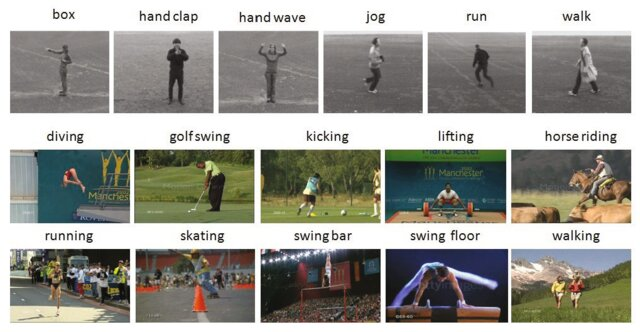
\includegraphics[width=0.8\textwidth]{sample_action_m1}}
	\caption{چندین نمونه از تصاویر فعالیت انسان
		\cite{tasvirAvalChapterYek}
	}
	\label{fig:humanActionM1}
\end{figure}
\subsection{تشخیص فعالیت از نقطه دید انسان}
زمانی که یک اتفاق یا فعالیت که عامل آن انسان است و انسان در به وقوع پیوستن آن عمل نقش دارد را مشاهده می‌کنیم، اولین عاملی که به آن توجه می‌کنیم خود شخص یا موقعیت بدنی شخص است. موقعیت بدنی به عنوان اولین عامل در توجه ما به آن فعالیت یا عمل نقش دارد.

عامل دومی که توجه انسان به آن جلب می‌شود، اشیاء مرتبط با انسان است. برای مثال ممکن است لیوانی که شخص در دست گرفته به ما این مفهوم را القا کند که شخص درحال نوشیدن است. پس اشیاء در فهمیدن یک عمل نقش بسیار مهمی دارند.

عامل بعدی که ناخودآگاه به آن توجه می‌شود، ژست شخص است. برای مثال شخصی درحال دویدن یک ژست و نحوه ایستادن خاصی دارد که انسان با یک نگاه متوجه فعالیتی که شخص درحال انجام آن است می‌شود. این عامل به خصوص در تشخیص فعالیت های ورزشی بسیار مهم است.

شبکه های عصبی عمیق از دل ساختار مغز انسان بیرون آمده و رشد کرده اند. پس طبیعی است که این طرز دید انسان می‌تواند در شبکه های عصبی جای گیرد و باعث شود شبکه درک بهتری از فعالیت داشته باشد. بنابراین از این سه عامل به عنوان عوامل اصلی تشخیص فعالیت انسان در شبکه های عصبی بهره برده می‌شود.

\section{انواع فعالیت های انسان}

فعالیت های انسان به ارتباط بین اشخاص، تعامل با اشیاء و محیطی که درآن زندگی می‌کنیم ربط پیدا می‌کند. این فعالیت ها به اعضای بدن یا حرکات کل بدن اشاره دارد و از چندین عمل ابتدایی که به ترتیب متوالی زمانی انجام می شوند تشکیل شده است. آنها می‌توانند توسط یک فرد یا گروهی از افراد انجام شوند. در این بخش سلسله مراتبی از فعالیت‌های انسانی را بسته به پیچیدگی آنها ارائه می‌شود که از اقدام ساده به رویدادهای پیچیده‌تر مقیاس بندی شده است. شکل
\ref{fig:kinds_human_acions}
این سلسله مراتب را نشان می دهد.

\vspace{8pt}
\begin{figure}[ht]
	\centerline{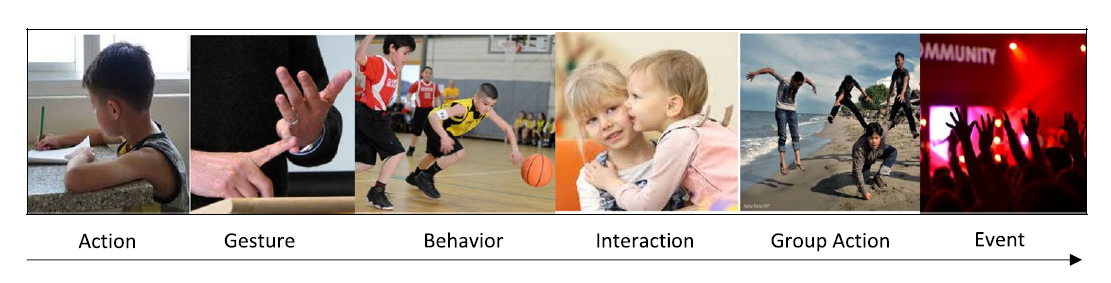
\includegraphics[width=0.8\textwidth]{kinds_human_acions}}
	\caption{انواع فعالیت های انسان از آسان به پیچیده (چپ به راست)
		\cite{HumanActionReviewMogadame}
	}ُ
	\label{fig:kinds_human_acions}
\end{figure}
\begin{itemize}
	\item \textbf{فعالیت اولیه انسان}\\
این شامل فعالیت‌های ساده است که نشان‌دهنده حرکات ارادی و/یا عمدی بدن است که مبنایی برای ایجاد سایر اقدامات پیچیده‌تر مانند «بالا بردن دست چپ» یا «راه رفتن» است. تشخیص این فعالیت ها آسان است و در ابتدا حول این نوع فعالیت ها،‌ تحقیق های زیادی صورت گرفت.
	
	\item \textbf{ژست}\\
 به طور معمول، ژست بخشی از ارتباط غیرکلامی است که می تواند برای بیان ایده ها یا دستورات مهم به کار رود. ژست‌ها نوع دوم فعالیت‌هایی هستند که ممکن است آگاهانه مانند «تشویق کردن» و ناخودآگاه مانند «پنهان کردن صورت با دست هنگام خجالتی شدن» یا «بیرون کشیدن دست هنگام لمس مواد داغ» باشند. برخی از ژست ها جهانی هستند، در حالی که برخی دیگر به زمینه های اجتماعی و فرهنگی کاملاً خاص مربوط می شوند. 
 
 \vspace{10pt}
	\item \textbf{رفتارها}\\
 مجموعه ای از کنش ها و واکنش های فیزیکی افراد در موقعیت های خاص را که از بیرون قابل مشاهده است و با عواطف و حالات روانی آنها مرتبط است، توصیف می کند.

	\item \textbf{فعالیت تعاملی}\\
کنش‌ها یا مبادلات متقابل بین دو نهاد یا بیشتر هستند که رفتار افراد یا اشیاء درگیر در تعامل را تغییر می‌دهند. آنها به طور کلی دو نوع فعالیت پیچیده هستند: انسان به انسان مانند "بوسیدن" یا انسان به شی مانند "آشپزی" که شامل ظروف مختلف در آشپزخانه است.

	\item \textbf{فعالیت گروهی}\\
 فعالیت هایی را تشکیل می دهد که توسط گروهی از افراد انجام می شود مانند "نوازش کردن". این فعالیت ها کم و بیش پیچیده هستند و شناسایی یا تشخیص آنها به دلیل وجود افراز زیاد و شلوغی، دشوار است. 

\end{itemize}

\section{تحلیل موقعیت بدنی در تشخیص فعالیت انسان} 

تحلیل موقعیت بدنی، به عنوان یکی از عوامل اصلی در تشخیص فعالیت انسان در تصاویر، اطلاعات غنی و بی‌نظیری را ارائه می‌دهد. این تحلیل نه تنها موقعیت دقیق دست‌ها و پاها را نشان می‌دهد بلکه به تحلیل زاویه و جهت این اجزاء ارزشمند نیز می‌پردازد. به عبارت دیگر، اطلاعات به دست آمده از تحلیل موقعیت بدنی می‌توانند نقش بسیار موثری در تفسیر رفتار و فعالیت‌های انسانی ایفا کنند.

بررسی مکان قرارگیری پاها و نحوه ایستادن یا حرکت نیز از اهمیت ویژه‌ای برخوردار است. این تحلیل می‌تواند بیشتر اطلاعاتی راجع به نوع فعالیت، مثل ایستادن در یک جا یا حرکت به سمت یک هدف، ارائه دهد. زاویه پاها نیز می‌تواند تصویر کلانی از حرکت انسان در یک لحظه خاص را ارائه کند و به تمیز بین افراد کمک کند.

علاوه بر این، تحلیل موقعیت بدنی به شناخت زاویه و جهت دست‌ها نیز کمک می‌کند. این اطلاعات می‌توانند نشان دهنده اهمیت و چگونگی حرکت دست‌ها باشند، مانند نگه داشتن یک شیء، انجام حرکات آزاد یا انجام حرکات خاص. این اطلاعات ممکن است از انواع فعالیت‌های روزمره مانند نوشیدن یا دست‌کاری با اشیاء گرفته تا فعالیت‌های پیچیده‌تر مثل ورزش‌های ویژه باشد.

نیاز به ترکیب تحلیل موقعیت بدنی با سایر عوامل مانند ژست‌ها و اشیاء از اهمیت خاصی برخوردار است. این ترکیب می‌تواند تفسیرهای دقیق‌تری از رفتار انسانی در تصویر فراهم کند.

در نهایت، تحلیل موقعیت بدنی، با ترکیب اطلاعات مکانی و حرکات اجزاء بدن، به شبکه‌های عصبی عمیق این امکان را می‌دهد تا با دقت بیشتری اقدام به تشخیص فعالیت‌های انسانی در یک تصویر نماید. این تحلیل نه تنها به ارتقاء دقت تشخیص بلکه به بهبود درک از رفتار انسان و نقش آن در تصویر کمک می‌کند.
\section{تحلیل اشیاء مرتبط با انسان در تشخیص فعالیت انسان}
تحلیل اشیاء مرتبط با انسان در تصاویر اطلاعات مهمی را در ارتباط با نوع فعالیت و تعامل انسان با محیط اطراف ارائه می‌دهد. این تحلیل با بررسی نوع و ویژگی‌های اشیاء، امکان تفسیر دقیق‌تر و سودمندتری از فعالیت درحال‌ انجام را فراهم می‌کند. برای مثال، ویژگی‌های یک لیوان در دست انسان می‌تواند نشان‌دهنده فعالیت نوشیدن باشد، در حالی‌که حضور یک دستگاه ورزشی نشان‌دهنده فعالیت ورزشی می‌باشد.
\subsection{تحلیل مکان قرارگیری اشیاء}
ارتباط مکانی اشیاء با انسان نقش اساسی در تعیین تفاوت‌ها و ارتباطات بین انسان و محیط دارد. بررسی مکان وضعیت اشیاء می‌تواند نشان‌دهنده تفصیلاتی از تعاملات و ارتباطات آنها با محیط باشد. به عنوان مثال، حضور یک شال در دست انسان ممکن است نشانگر فعالیتی خاص باشد، مانند خروج در هوای سرد.
\subsection{تمایز بین اشیاء مختلف}
تمایز بین اشیاء مختلف اطلاعات ارزشمندی از نوع و تأثیر اشیاء بر فعالیت انسان ارائه می‌دهد. این تمایز می‌تواند نقش بسزایی در تحلیل تعاملات و تفسیر اثرات مختلف اشیاء داشته باشد. به عنوان مثال، تفاوت میان یک کتاب و یک دستگاه موبایل در دست انسان.
\subsection{ارتباط با اعمال انسان}
بررسی تأثیر اشیاء بر اعمال انسان می‌تواند ما را به سوی درک بهتری از نحوه استفاده و تأثیر اشیاء بر رفتار انسان هدایت کند. این تحلیل می‌تواند نشان‌دهنده نقش یک ابزار ورزشی یا اشیاء کاری باشد که تعامل آن با انسان در تصویر نمایان است.
\subsection{تداخل با اجزاء بدن}
تداخل و تعامل اشیاء با اجزاء بدن اطلاعات اضافی را فراهم می‌کند. این تحلیل می‌تواند ما را به درک بهتری از نحوه استفاده انسان از اشیاء و تأثیر آن بر حرکات بدن هدایت کند. به عنوان مثال، نحوه نگه‌داشتن یک فنجان در دست انسان.
\subsection{ارتباط با دیگر عوامل}
ترکیب تحلیل اشیاء مرتبط با انسان با دیگر عوامل مانند موقعیت بدنی و ژست‌ها امکان تفسیر دقیق‌تر و جامع‌تری از رفتار انسان در تصویر را فراهم می‌کند. این ترکیب می‌تواند به بهبود دقت در تشخیص فعالیت‌های انسانی در تصاویر کمک کند.

تحلیل اشیاء مرتبط با انسان نیز با در نظر گرفتن نقش اشیاء در محیط اطراف انسان، به شبکه‌های عصبی عمیق این امکان را می‌دهد تا با دقت بیشتری نوع فعالیت‌ها و تعاملات انسان با اشیاء را در یک تصویر تشخیص دهد. این تحلیل به گسترش دامنه تفسیر و تشخیص تصاویر کمک کرده و در درک بهتر از فعالیت‌های انسانی در محیط اطراف را نشان می‌دهد. همچنین این تحلیل ما را به سوی یک نگرش جامع تر نسبت به رفتارهای انسانی هدایت می‌کند و اطلاعات ارزشمندی را از جنبه‌های مختلف فیزیکی و روانی ارائه می‌دهد. با پیشرفت تکنولوژی و توسعه الگوریتم‌های هوش مصنوعی، تحلیل ژست‌ها می‌تواند به یک ابزار مؤثر در زمینه‌های مختلف از پزشکی تا رابط‌های کاربری تبدیل شود.
\section{تحلیل ژست در تشخیص فعالیت انسان}
ژست‌ها به عنوان یک جنبه اساسی در تشخیص فعالیت انسان از اهمیت بالایی برخوردارند. تحلیل دقیق این ژست‌ها به ما امکان می‌دهد تا نه تنها نوع فعالیت انسان را شناسایی کنیم بلکه درک عمیق‌تری از رفتارهای جسمی و ذهنی او نیز پیدا کنیم. در ادامه به بررسی اجمالی از تحلیل ژست در تشخیص فعالیت انسان می‌پردازیم و مراحل مختلف این تحلیل را معرفی می‌کنیم.
\subsection{تفکیک ژست‌ها بر اساس نوع فعالیت}
تحلیل ژست‌ها بر اساس نوع فعالیت انسان ابتدا با شناخت پتانسیل پیام‌های مختلف این ژست‌ها شروع می‌شود. به عبارت دیگر، این بخش از تحلیل به درک چگونگی انتقال اطلاعات در جهت تشخیص نوع فعالیت کمک می‌کند. به عنوان مثال، ژستی که به همراه یک وسیله ورزشی صورت گیرد، اطلاعاتی از نوع ورزش درحال انجام را منتقل می‌کند.
\subsection{تحلیل جنبه‌های حرکتی ژست}
در این مرحله، جنبه‌های حرکتی ژست‌ها با دقت بیشتری مورد بررسی قرار می‌گیرند. سرعت، نحوه انجام حرکات، و حتی نقاطی که در طول ژست تاکید شده‌اند، اطلاعات مفیدی در خصوص نحوه اجرای فعالیت انسانی را ارائه می‌دهند. برای مثال، ژست با حرکات متنوع و شتاب‌دار ممکن است به فعالیت ورزشی یا فعالیت‌های پویا اشاره داشته باشد.

\subsection{تحلیل انعکاس ژست در فعالیت}

این مرحله به بررسی انعکاس‌های روحی و فیزیکی ژست‌ها می‌پردازد. انعکاس‌های روحی می‌توانند در بیان حالت هیجانی، شادابی یا حتی استرس شخصیت انسان تاثیرگذار باشند. انعکاس‌های فیزیکی نیز ممکن است جزئیاتی از سلامت و نشاط بدنی را نمایش دهند. این تحلیل به ما کمک می‌کند تا فراتر از سطح ژست، به اطلاعات ضمنی در مورد فعالیت انسانی دست یابیم.

\subsection{تحلیل معناشناسی ژست‌ها}

در این بخش، تحلیل معناشناسی ژست‌ها بیشتر به افق‌های فرهنگی و ارتباطات اجتماعی گسترده می‌شود. هر ژست ممکن است پیام‌های زیادی ارسال کند که باید در سیاق فرهنگ و محیط اجتماعی قرار گیرد. مثلاً، یک ژست معین ممکن است در یک جامعه به معنای احترام و در دیگر جا به معنای خوشحالی باشد. درحالی که درتصویر نمی‌توان تمایزی بین این ها قائل شد لذا این یک عامل انحرافی در شناسایی فعالیت می‌تواند به شمار برود.

\subsection{تفاوت‌ها در ژست‌ها بر اساس فرهنگ}

در این مرحله، تحلیل تفاوت‌های فرهنگی در تشخیص ژست‌ها بررسی می‌شود. هر جامعه و فرهنگ ممکن است ژست‌ها را با تفاوت‌های معنایی خود تفسیر کند. این بررسی به ما کمک می‌کند تا در طراحی سیستم‌های تشخیص ژست، به تفاوت‌های فرهنگی توجه کنیم و جلوی ابهامات در تفسیر ژست‌ها را بگیریم.

\begin{itemize}
	\item
	حال ترکیب سه عامل موقعیت بدنی، اشیاء مرتبط با انسان و ژست به ما این امکان را می‌دهد تا یک تحلیل جامع از فعالیت انسانی داشته باشیم. برای مثال اگر شخصی با یک لیوان در دست، در موقعیت بدنی که نشانگر نشستن است و با ژستی که به حرکات آرامشی اشاره دارد، را مشاهده کنیم، می‌توانیم به احتمال زیاد نتیجه بگیریم که او در حال نشسته و در حال لذت بردن از یک نوشیدنی است. این ترکیب اطلاعات از موقعیت بدنی، اشیاء مرتبط با انسان و ژست به ما اطلاعات دقیق‌تر و گسترده‌تری از فعالیت انسانی ارائه می‌دهد. 
\ref{fig:human_three_amel_mog}
دو نمونه از ارتباط موقعیت بدنی، اشیاء مرتبط و ژست را در فهم فعالیتی که در حال انجام است، نشان می‌دهد. در تصویر سمت  راست"لپ تاپ" و "موس" به عنوان اشیاء، "طرز نشستن افراد" به عنوان ژست و کل ناحیه بدن شخص به عنوان یک موقعیت بدنی نشان می‌دهد که درحال کار با لپ تاپ هستند. در تصویر سمت چپ نیز "لیوان" در تشخیص فعالیت "نوشیدن" و طرز نگه داشتن لیوان در دست نشان می‌دهد که فقط لیوان در دست دارند و درحالی نوشیدن نیستند. پس ژست در اینجا یک عامل کمک کننده است.
\end{itemize}
\vspace{8pt}
\begin{figure}[ht]
	\centerline{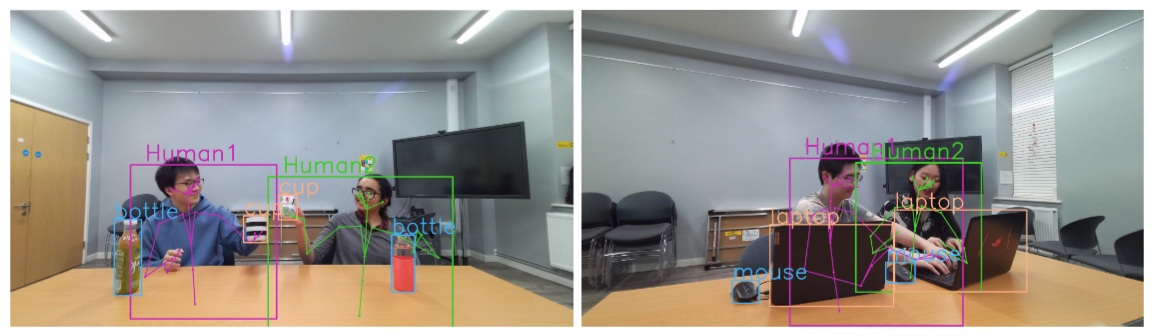
\includegraphics[width=0.8\textwidth]{human_three_amel_mog}}
	\caption{دو نمونه تصویر از تأثیر سه عامل ژست، اشیاء و موقعیت انسان در درک فعالیت
		\cite{tasvirSevomChapterYek}
	}ُ
	\label{fig:human_three_amel_mog}
\end{figure}
\vspace{20pt}

\section{شبکه‌های عصبی عمیق و تشخیص فعالیت انسان در تصویر}

\gls{DeepNeuralNetworks}
 یکی از مفاهیم مهم در زمینه %
\gls{DeepLearning}
  هستند. این ایده از تلاش برای شبیه‌سازی عملکرد مغز انسان و افزایش توانایی یادگیری ماشین در حضور داده‌های بزرگ مشتق شده است.

شبکه‌های عصبی عمیق از ابتدا ایده‌آل محسوب نمی‌شدند ولی با پیشرفت‌های در حوزه پردازش تصویر و صوت، افزایش توانایی محاسباتی، و استفاده از الگوریتم‌های بهبود یافته در آموزش شبکه‌ها، معماری عصبی عمیق به یک ابزار قدرتمند برای حل مسائل یادگیری ماشین تبدیل شده است.

شبکه‌های عصبی عمیق می‌توانند به صورت خودکار و بدون نیاز به تعریف دستی از ویژگی‌ها، اطلاعات مهم را از داده‌ها استخراج کرده و الگوهای مختلف مرتبط با فعالیت‌های انسانی را تشخیص دهند. این مزیت از اهمیت زیادی در حوزه تشخیص و تفسیر تصاویر می‌باشد.

به عنوان مثال، در تشخیص فعالیت انسان در تصاویر، این شبکه‌ها می‌توانند به طور خودکار اجزای مرتبط با افراد، اشیاء، حرکات، و موقعیت‌های مکانی را تشخیص داده و اطلاعات بهتری برای تصمیم‌گیری در مورد نوع فعالیت انسانی فراهم کنند.
استفاده از شبکه‌های عصبی عمیق در این حوزه امکانات جدیدی را برای تحقیقات و کاربردهای عملی فراهم کرده و می‌تواند بهبود قابل توجهی در دقت و کارایی مدل‌ها برای تشخیص فعالیت انسان در تک تصویر داشته باشد. شکل %
\ref{fig:neural_network_action_first}
یک نمونه از چارچوب شبکه عصبی عمیق برای تشخیص فعالیت انسان است. البته دراینجا ورودی چندین سیگنال از فعالیت‌های مختلف است که به شبکه عصبی عمیق داده شده است. درکاربرد مشابه می‌توان ورودی را یک تصویر نیز درنظر گرفت.
\begin{figure}[ht]
	\centerline{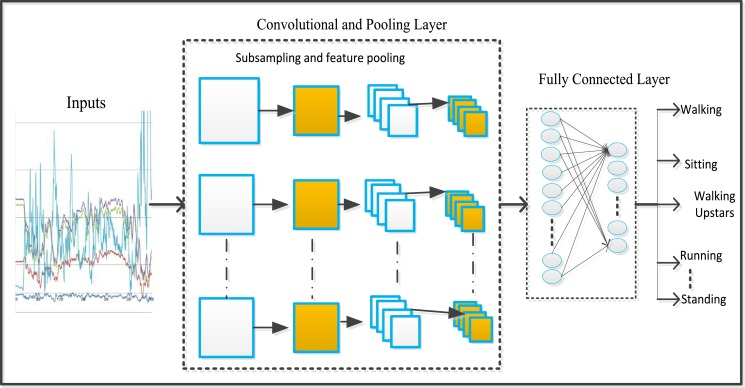
\includegraphics[width=0.7\textwidth]{neural_network_action}}
	\caption{
		مثالی از یک چارچوب شبکه عصبی عمیق برای تشخیص نوع فعالیت
		\cite{WinNT}
	}
	\label{fig:neural_network_action_first}
\end{figure}

در این پایان‌نامه، ما با بهره‌مندی از نقش شبکه‌های عصبی عمیق در فرایند تشخیص فعالیت انسان در تک تصویر به طراحی شبکه و الگوریتم جهت تشخیص فعالیت انسانی، اقدام خواهیم کرد. در زیر به یک سری از مزیت های مهم شبکه‌های عصبی عمیق اشاره شده است:
\begin{itemize}
	\item \textbf{پیچیدگی معماری شبکه‌های عصبی عمیق:}\\
از معماری‌های مختلف شبکه‌های عصبی در این زمینه استفاده می‌شود. معماری مناسب با ویژگی‌های فعالیت‌های انسانی در تصاویر انتخاب و بهینه‌سازی می‌شود. معماری کانوولوشنی%
\LTRfootnote{Convolutional Neural Networks (CNN)}
اغلب در این کاربرد به دلیل استخراج ویژگی‌های متفاوت در سطوح مختلف، مورد استفاده قرار می‌گیرد. 

	\item \textbf{آموزش با مجموعه داده متنوع:}\\
آموزش شبکه‌های عصبی عمیق با استفاده از مجموعه داده‌های متنوع و جامع از تصاویر مختلف، از جمله فعالیت‌های انسانی در شرایط مختلف، اطمینان از عملکرد مدل در شرایط واقعی را افزایش می‌دهد.

\item \textbf{قابلیت یادگیری از داده‌های پیچیده:}\\
شبکه‌های عصبی عمیق به عنوان یک الگوریتم یادگیری ماشین با قابلیت یادگیری از داده‌های پیچیده شناخته می‌شوند. این بدان معناست که با تغییرات در شرایط نورپردازی، زاویه دید، وضوح، و تنوع دیگر در تصاویر، این شبکه‌ها قادرند الگوها و ویژگی‌های مفید را به صورت خودکار استخراج کنند.
\end{itemize}

\section{شبکه ترنسفرمر و مکانیزم توجه}

شبکه‌های ترنسفرمر یکی از معماری‌های بسیار قوی در زمینه یادگیری عمیق هستند که ابتدا برای پردازش دنباله‌ها (مثل متون) طراحی شدند.
\cite{AttentionIsAllNeed}
 اما در ادامه، نشان دادند که به عنوان یک راهکار کارآمد می‌توانند در حوزه تشخیص تصاویر و ویدئوها نیز مؤثر باشند. در داخل ترنسفرمر از %
\gls{AttentionMechanism}
استفاده می‌شود.
مکانیزم توجه به شبکه این امکان را می‌دهد تا توجه بیشتری به بخش‌های مهم تصاویر بدهد. این مکانیزم با محاسبه وزن‌های مختلف برای اجزای مختلف تصاویر، اطلاعات مهم را برجسته می‌کند. 

شبکه‌های ترنسفرمر به دلیل قابلیت بررسی دنباله‌های بلند و انتقال اطلاعات بین ورودی‌ها، در تشخیص الگوهای پیچیده مانند فعالیت‌های انسانی در تصاویر مؤثر هستند. این شبکه‌ها با استفاده از لایه‌های توجه، می‌توانند بهترین ویژگی‌ها را از تصاویر استخراج کرده و تمرکز را به بخش‌های مهمتر تصویر معطوف نمایند.

با استفاده از این مکانیزم توجه، حساسیت به جزئیات فعالیت‌های انسانی در تصاویر بهبود یافته و اطلاعات دقیق‌تری در فرآیند تشخیص مورد استفاده قرار می‌گیرد.
شکل%
\ref{fig:transformer_whole_struc}
 ساختار شبکه ترنسفرمر که در کاربرد متن معرفی شده است را نشان می‌دهد. شکل%
\ref{fig:self_attention_struc}
 ساختار
\gls{Self-Attention}
که به عنوان بخش اصلی ترنسفرمر شناخته می‌شود را نشان می‌دهد. هدف از ساختن این نوع معماری مقایسه دوتا بردار باهم است که مشخص شود این دو بردار چقدر با یکدیگر تشابه دارند و به همان میزان باهمدیگر ترکیب شوند تا خروجی معنادار و ارتباط‌دهی شده تولید کند.
\begin{figure}
	\centering
	
	\subfloat[شکل کامل از یک شبکه ترنسفرمر]{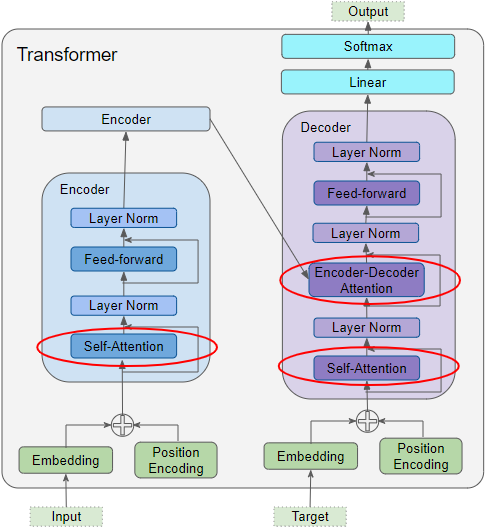
\includegraphics[width=0.5\textwidth]{transformer_whole_struc}\label{fig:transformer_whole_struc}}
	\hfill
	\subfloat[Attention Self داخل ترنسفرمر]{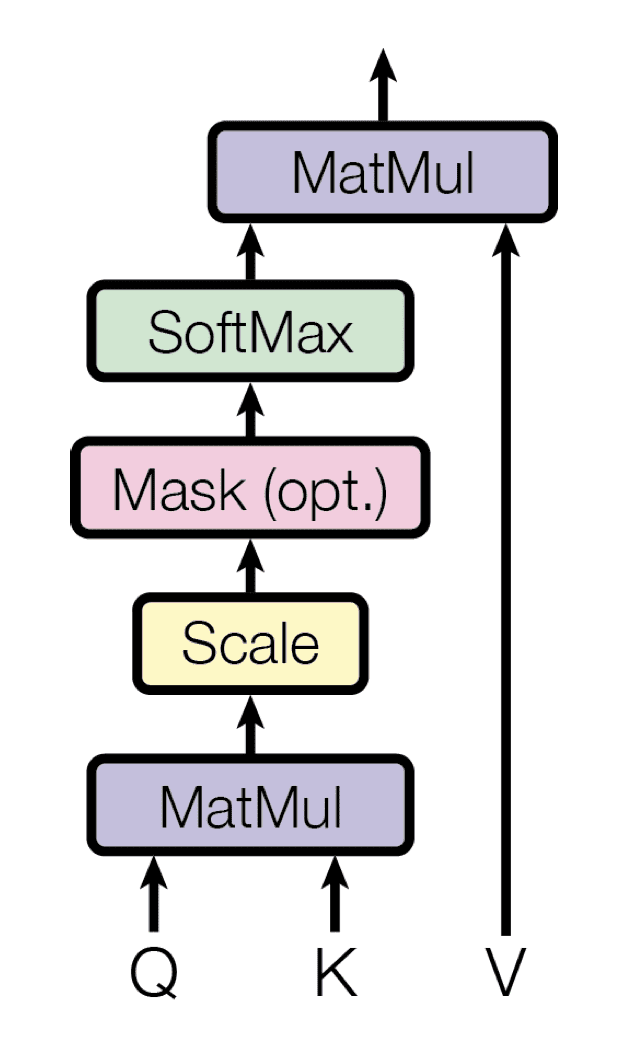
\includegraphics[width=0.3\textwidth]{self_attention_struc}\label{fig:self_attention_struc}}
	
	\caption{ساختار کلی شبکه ترنسفرمر و مکانیزم توجه
		\cite{AttentionIsAllNeed}
	}
	\label{fig:mainfigure}
\end{figure}

\subsection{بهره‌مندی از معماری \gls{Self-Attention}}

از مکانیزم %
\gls{Self-Attention}
 به عنوان یک ابزار قوی برای تحلیل و استخراج ویژگی‌های تصاویر به منظور شناسایی فعالیت‌های انسانی نیز استفاده می‌شود.
\gls{Self-Attention}
یکی از عناصر اصلی معماری ترنسفرمرها است که توانایی بررسی تمام نقاط ورودی را دارد و در فرایند تصمیم‌گیری بر روی این نقاط تأکید می‌کند.
\gls{Self-Attention}
یک رویکرد در یادگیری عمیق است که به شبکه‌ها این امکان را می‌دهد تا با توجه به اهمیت نقاط مختلف ورودی، وزن‌های مختلفی را به آن‌ها تخصیص دهند.
در مدل %
\gls{Self-Attention}
،هر نقطه ورودی با ویژگی‌های مختلفی از نقاط دیگر ترکیب می‌شود و این امر اطلاعات بسیار غنی‌تری را برای هر نقطه فراهم می‌کند.

\begin{itemize}
	\item \textbf{عملکرد \gls{Self-Attention}در شناسایی فعالیت‌های انسانی}\\
\gls{Self-Attention}
 این امکان را فراهم می‌کند تا شبکه به صورت هوشمندانه بر روی نقاط مهم تصاویر تمرکز کند. این ویژگی می‌تواند در شناسایی افراد، اشیاء، و حرکات مرتبط با فعالیت‌های انسانی بهبود بخشیده و به دقت مدل کمک کند.\\
 همچنین %
\gls{Self-Attention}
  به شبکه این امکان را می‌دهد تا اطلاعات را به صورت همزمان از تمام فضای زمانی تصویر درنظر بگیرد. این ویژگی می‌تواند در تشخیص فعالیت‌های زمانی و توالی‌های مرتبط با انسان کمک کننده باشد. البته چون فعالیت های قابل شناسایی در تک تصویر هستند، به جای توالی‌های زمانی ورودی های دیگری که از تصویر به دست می‌آید را درنظر خواهیم گرفت.
  	\item \textbf{آموزش \gls{Self-Attention}}\\
	\gls{Self-Attention}
  با استفاده از مجموعه داده‌های بزرگ و متنوع، می‌تواند الگوها و اطلاعات مرتبط با فعالیت‌های انسانی را یاد بگیرد. استفاده از یادگیری انتقالی و بهره‌گیری از مدل‌های از پیش‌آموزش دیده شده نیز می‌تواند به بهبود یادگیری در موارد مشابه کمک کند.
    	\item \textbf{ترکیب \gls{Self-Attention} با شبکه های عصبی عمیق}\\
	\gls{Self-Attention}
 به عنوان یک عنصر اصلی در مدل‌های ترنسفرمر، به شبکه‌های عصبی عمیق این امکان را می‌دهد تا در فرایند تصمیم‌گیری و شناسایی فعالیت‌های انسانی از اطلاعات بهتری بهره‌مند شوند.
 ترکیب %
   \gls{Self-Attention}
  با شبکه‌های عصبی عمیق می‌تواند توانایی مدل را در درک و تفسیر تصاویر افزایش دهد و دقت در تشخیص فعالیت‌های انسانی را بهبود بخشد.
\end{itemize}
\section{اهداف پژوهش}
هدف این پایان نامه با درنظر گرفتن موارد گفته شده، تشخیص فعالیت انسان در تصویر می‌باشد که اطلاعات جانبی تصویر در روند تشخیص بکار گرفته می‌شود. این اطلاعات شامل اشیاء مرتبط با فعالیت، ژست انسان و موقعیت بدنی انسان که ناحیه کامل انسان را پوشش است.

در بخش ابتدایی از یک شبکه استفاده می‌شود که ویژگی‌های موجود درتصویر را استخراج کند. این ویژگی‌ها در تعامل با مختصات اشیاء، مختصات ژست و مختصات موقعیت بدنی در یک شبکه ترنسفرمر ترکیب می‌شود که ویژگی‌های مرتبط بهتر مشخص شود. برای توصیف بهتر ژست از مسیر توصیف کننده زاویه بدن استفاده می‌شود که یک بردار توصیف کننده از زاویه اعضای بدن انسان است که یک بردار ویژگی از استخوان بندی بدن را نشان می‌دهد. این مسیر یک مسیر کمک کننده برای شبکه است که از ویژگی‌های نهفته ژست علاوه بر ویژگی‌های ظاهری نیز استفاده شود. هدف نهایی این است که ژست را به نوعی در تشخیص فعالیت دخالت دهیم.

درنهایت مرتبط‌ترین شیء و مرتبط‌ترین ناحیه بدن از ژست انتخاب می‌شود و با خروجی موقعیت بدنی ترکیب می‌شود و یک تشخیص از فعالیت درحال انجام صورت می‌گیرد. پس ورودی شبکه یک تک تصویر و خروجی نهایی یک بردار به طول تعداد دسته‌های موجود در هر مجموعه داده می‌باشد و بسته به تعداد دسته‌بندی‌های مجموعه داده تغییر خواهد کرد. 

ممکن است در برخی از تصاویر کل بدن انسان مشخص نباشد و اصطلاحاً انسداد رخ دهد که کار تشخیص اعضای بدن انسان را برای تشخیص ژست مشکل می‌کند. برای غلبه براین چالش از ناحیه‌های در دسترس انسان استفاده می‌شود که شبکه ورودی بدون مقدار نداشته نباشد که باعث گمراهی شبکه حین آموزش شود. همچنین شرایط نوری در هرتصویر متفاوت است و ممکن است ناحیه انسان به طور واضح قابل دیدن نباشد، بنابراین یک سری پیش پردازش ها جهت بهبود تصویر انجام می‌شود.

برخی مواقع نیز ممکن است مجموعه داده کافی دردسترس نباشد و شبکه با تکرار آموزش روی این مجموعه داده به سمت بیش برازش حرکت کند. درچنین حالتی استفاده از افزایش داده مقداری نتیجه را بهبود می‌دهد و همچنین باعث می‌شود شبکه تنوع تصاویر بیشتری به خود ببیند.
\section{سوالات پژوهشی} 
\begin{enumerate}
	\item 
	آیا استفاده از یک شبکه ترنسفرمر در تعامل با مسیر توصیف کننده برای ژست، می‌تواند با استفاده از مختصات ژست مدل مناسبی برای تشخیص فعالیت انسان باشد؟
	\item
	با توجه به چالش‌های شناسایی نقاط کلیدی بدن در تک تصاویر، کدام یک از نقاط کلیدی انسان در شناسایی ژست تاثیر کمتری داشته و می‌‌تواند نادیده گرفته شود؟
	\item
	آیا استفاده از ژست انسان و ترکیب آن با ویژگی ظاهری انسان می‌تواند منجربه افزایش دقت در شناسایی نوع فعالیت انسان گردد؟
	\item
	آیا استفاده از اطلاعات مکانی اشیاء و موقعیت و نوع آنها نسبت به مکان انسان در تصویر می‌تواند منجر به افزایش دقت در شناسایی نوع فعالیت انسان گردد؟
\end{enumerate}
\section{جمع بندی و ارائه راهکار پیشنهادی} 

طبق مواردی که گفته شد هدف این پایان نامه، تشخیص نوع فعالیت انسان در تصویر است. در تصویر به دلیل نبودن اطلاعات زمانی شناسایی عمل چالش هایی دارد. گفتیم که انسان به صورت ذاتی می‌تواند بسیاری از فعالیت‌های درحال انجام را حتی از روی تصویر تشخیص دهد.

سپس به انواع فعالیت‌های انسانی پرداختیم که سطح بندی های متفاوتی دارد. از فعالیت های اولیه که شامل حرکات ابتدایی انسان مانند راه رفتن،‌ دویدن و... است، تا در آخر که فعالیت های پیچیده مانند یک مهمانی که درافراد زیادی در به وقوع پیوستن این فعالیت مشارکت دارند، اشاره شد.

درادامه به نحوه تشخیص فعالیت های انسانی از روی موقعیت بدنی شخص، اشیاء مرتبط با انسان و ژست شخص قابل شناسایی است،‌ پرداخته شد و انواع آنها نام برده شد و ترکیب اشیاء، ژست و موقعیت بدنی انسان برای تشخیص فعالیت درنظرگرفته شد. شبکه های عصبی و مکانیزم توجه به صورت مختصر توضیح داده شد که به چه صورت در کاربرد شناسایی فعالیت می‌توان بهره‌مند شد.

تشخیص فعالیت انسان از روی تک تصویر،‌ یک مسئله %
\gls{Classification}
 محسوب می‌شود بنابراین از بیشتر الگوریتم ها و ارزیابی‌های مرتبط با طبقه‌بندی دراین کار استفاده می‌شود. معماری پیشنهادی در این پایان استفاده از یک شاخه‌ی دیگر از %
 \gls{Self-Attention}
  به منظور ترکیب ویژگی‌های موقعیت بدنی با ژست انسان است. در این حالت اجزای بدن به صورت جداگانه با کل تصویر فرد ترکیب می‌شود و شبکه به یک درکی از ژست می‌رسد که در شناسایی فعالیت تاثیرگذار است.
  
 به دلیل محدود بودن سیستم محاسباتی و طولانی بودن زمان آموزش و همچنین پیچیدگی محاسباتی زیاد تشخیص فعالیت در ویدیو،‌ ما سراغ تشخیص فعالیت در تک تصویر رفتیم. هدفمان این است که از داده‌ها و اطلاعات موجود استفاده کنیم تا نشان دهیم ترکیب ژست با عواملی مانند موقعیت بدنی چه نتایجی می‌تواند داشته باشد و آیا درنظر گرفتن این فاکتور موجب افزایش دقت می‌شود یا نه.

\section{ساختار پایان نامه} 

فصل دوم مروری از کارهایی که در این زمینه انجام شده، بررسی می‌شود و به بررسی چهار زیرشاخه اساسی از تشخیص تصویر محور پرداخته شده است.

پس از بررسی کارهای گذشته، در فصل سوم روش پیشنهادی بررسی می‌شود. دراین مرحله از پیش پردازش‌ها شروع شده و پس از بررسی آنها به دو روش اصلی استفاده از ژست پرداخته می‌شود و هرکدام از آنها را در قالب یک بخش جداگانه بررسی می‌کنیم.

در فصل چهارم نتایجی که از ارزیابی روش پیشنهادی درمقایسه با یک سری کارهای اصلی گزارش می‌شود. روی دو نمونه از مجموعه ‌داده‌هایی که اغلب در این خوزه کاربرد دارند تست و اجزا می‌شود و نتایج هرکدام در بخش جداگانه گزارش می‌شود.

در فصل آخر نیز به نتیجه‌گیری نهایی و پیشنهادات برای کارهای آتی پرداخته می‌شود.

		% فصل اول: مقدمه
% !TeX root=../main.tex
\chapter{مروری بر کارهای گذشته}

\section{مقدمه}
در فصل اول مفاهیم پایه و اساسی در مسئله شناسایی فعالیت انسان در تک تصویر با استفاده از شبکه‌های عصبی عمیق و مکانیزم توجه مطرح و بررسی شد و توضیحات مختصری از هربخش داده شد. در این فصل تعدادي
از روش‌های شناسایی فعالیت شناخته شده در این حوزه بررسی شده است. در این فصل مقالات و
الگوریتمهایی که این پایان نامه در راستاي مسیر آنها پیش رفته است و ایده‌ي اصلی این تحقیق بر اساس این
روشها شكل گرفته است، به صورت کامل و با جزییات بیشتري توضیح داده شده است.
در نمودار %
\ref{fig:masir_asli_payan}
 الگوریتم‌های تشخیص فعالیت انسان تقسیم بندی شده است. دسته هایی که تحقیق حال حاضر در آن قرار گرفته با رنگ سبز رنگ مشخص شده اند.
\vspace{8pt}
\begin{figure}[ht]
	\centerline{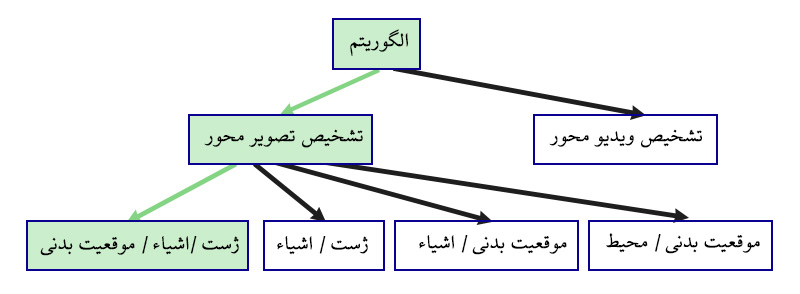
\includegraphics[width=0.8\textwidth]{masir_asli_payan}}
	\caption{دسته بندی الگوریتم های تشخیص فعالیت انسان}
	\label{fig:masir_asli_payan}
\end{figure}
%\vspace{12pt}

\section{تشخیص فعالیت  در تک تصویر}
مطابق با زمینه‌های دیگر در بینایی کامپیوتر، تشخیص فعالیت انسان در تک تصویر از روش‌های سنتی و دستی استخراج ویژگی تکامل یافته تا به روش‌های شبکه عصبی عمیق رسیده است.

در سال 2018 سرلا اس آر و همکارش %
\cite{ActionRec_using_Res_network}
از یک مدل شبکه عصبی عمیق برای کلاس‌‌بندی استفاده کرده اند. آنها بدون درنظر گرفتن هیچ یک از اصلاعات اضافی در تصویر که شامل محیط،‌ ژست و اشیاء می‌باشد، فقط به شکل یک مسئله کلاس‌بندی به موضوع نگاه کرده اند.

در سال 2019 سینا محمدی و همکارانش %
\cite{Ensemble_deep_neu_action_still}
 بهبودی بر شبکه های عصبی با نگاهی به مکانیزم توجه داشته اند. برای غلبه بر کم بود داده ها برای آموزش شبکه‌های کانولوشنی از روش %
\gls{EnsembleLearning}
  استفاده کرده اند. آنها از طریق %
\gls{TransferLearning}
مدل های آموزش دیده قبلی، به مدل های جدید خودشان بهبودی روی دقت داشته اند. همچنین از مکانیزم توجه برای یافتن ارتباط بین اجزای تصاویر در داخل ساختار مدل استفاده شده که موجب افزایش دقت شده است.
 
 در سال 2020 سید سجاد اشرفی و همکارانش %
 \cite{Knowledge_dist_recognition}
 از شبکه %
 \gls{Teacher-Student}
 که جزء روش های %
\gls{KnowledgeDistillation}
 محسوب می‌شود، استفاده کرده اند. در اینکار از یک شبکه بزرگتر برای آموزش یک شبکه کوچکتر کمک گرفته اند. این کار آموزش شبکه کوچکتر را تسریع می‌کند و همچنین باعث می‌شود شبکه در ابتدا مسیر آموزش خود را بداند و از %
\glspl{Loss}
  بزرگ جلوگیری شود. در این کار وابستگی به %
\gls{BoundingBox}
  انسان یا اشیاء وجود ندارد و شبکه می‌تواند بدون درنظر گرفتن %
 \gls{BoundingBox}
   مسیر آموزش خود را طی کند.
  
  در سال 2021 حجت اصغریان و همکارانش %
  \cite{Still_image_action_ensemble}
  مدل یادگیری گروهی بهبود یافته ای که از مکانیزم توجه ویژگی محور بهره می‌برد،‌ استفاده کرده اند. آنها با درنظر گرفتن این واقعیت که مدل روی مجموعه داده‌های کوچکتر، اغلب نتیجه‌ی بهتری نیز می‌دهد، مجموعه داده را به 4 بخش تقسیم کرده اند سپس برای هر بخش یک شبکه کانولوشنی و دسته‌بند جدا درنظر گرفته اند.\\
در کنار این از مکانیزم توجه نیز بهره برده اند که این چهار تا بخش تقسیم شده از مجموعه داده، یکبار باهم مقایسه و ارتباط سنجی شود تا یک ویژگی ترکیب شده از اینها بدست بیاید.

در اغلب این مقالات که ذکر شد، توجه‌ی به ناحیه های کلیدی مانند انسان،‌ اشیاء و ژست به صورت یک بخش مکمل نشده است. اینکار مدنظر ما نیست چون منطقی به نظر نمی‌رسد که اطلاعات مفید تصویر را نادیده بگیریم. بدلیل نداشتن اطلاعات زمانی در تشخیص فعالیت تک تصویر، نادیده گرفتن این اطلاعات دقت تشخیص را کاهش خواهد داد. درهمین‌حین حضور اطلاعات نامرتبط مانند %
\gls{Background}
  و اشیاء نامرتبط منجربه گمراهی شبکه می‌شود.
  
  در سال 2022 پاوان و همکارش %
	\cite{action_sift_key_points}
	از SIFT %
	\LTRfootnote{Scale-Invariant Feature Transform}
	جهت یافتن نقاط کلیدی بدن انسان در تصویر استفاده کردند و از این نقاط بدست آمده برای تشخیص فعالیت بهره بردند.\\
برای شناسایی نقاط برجسته پایدار، تصویر اصلی را با یک تابع گوئسین%
	\LTRfootnote{Guasian}
	ترکیب کردند و لبه‌های مفید از ناحیه انسان را بدست آوردند. از این لبه‌های بدست آمده اطلاعات مهمی بدست ‌می‌آید که در تشخیص فعالیت موثر هستند.این لبه‌ها در تشخیص نقاط اطراف بدن انسان استفاده ‌می‌شود. در نهایت از نقاط کلیدی بدن انسان استفاده کردند تا فاصله اعضای بدن با یکدیگر را محاسبه کنند و درقالب یک بردار ویژگی در روند آموزش ازش استفاده کردند. دراینجا به دلیل استفاده از الگوریتم‌های یادگیری ماشین برای استخراج نقاط،‌ حجم پارامتر‌ها کاهش می‌یابد ولی درعوض دقت چندان مطلوبی بدست نیامده است.
	
	در سال 2023 محمد عبدالهادی %
	\cite{hum_action_behavior_transfer_learning}
	از یادگیری انتقال استفاده کرده است به شکلی که فقط بخشی از شبکه را آموزش دهد و بخش دیگری را قفل کند که وزن‌های مدل در روند آموزش به‌روز نشوند. دراین کار روی مجموعه داده‌ی که برای آموزش استفاده می‌شود بیشتر تمرکز کرده است.\\
	دراین مقاله از یک مجموعه داده‌ی که روی تشخیص فعالیت انسان در ویدیو کارکرد دارد استفاده کرده است و از فریم‌های ویدیو‌‌های این مجموعه داده به عنوان تصاویر جهت آموزش شبکه بهره برده است. درواقع از یک الگوریتمی استفاده کرده است که فریم‌های برتر را از مجموعه داده جدا کند و از آنها در آموزش شبکه استفاده کند. ضعف این مقاله در استفاده از مدل‌های قدیمی برای استخراج ویژگی به جای مدل‌های به روزتر مانند ResNet است.
	
	در سال 2023 آرناب دی و همکارانش %
	\cite{interactions_adaptive_drnet}
	در یک کار متفاوت روی ارتباط انسان با انسان را در یک فریم از ویدیو برای تشخیص فعالیت انسان کار کردند. آنها برای یافتن این ارتباط از یک ماژول توجه AdaptiveDRNet استفاده کردند. سه عدد از این ماژول ها پشت سرهم در داخل بخش استخراج ویژگی قرار دارند تا ترکیب ویژگی‌ها به خوبی صورت گیرد. همچنین در بین لایه‌‌ها از تابع فعال‌ساز Swish استفاده شده است که اصولا همچین تابع فعال‌سازی در اغلب کارها مشاهده نمی‌شود. البته نتایج روی مجموعه ‌داده‌ی %
	\lr{Stanford40}
	چندان رضایت بخش نیست.
	
	در سال 2023 شوآنگ لی یانگ و همکارانش %
	\cite{patch_boxless_action}
	مدلی طراحی کردند که بی نیاز از %
	\glspl{BoundingBox}
	اشیاء و انسان باشد. آنها با قطعه‌بندی تصویر سعی کردند که مدل را طوری آموزش دهند که از خود تصویر اطلاعات ناحیه‌ای که اشیاء یا انسان درآن قرار دارد را درک کند. مراحل استفاده از دو مسیر تشکیل شده است. در مسیر اول ماژول تحریک فعالیت روی کل تصویر اعمال می‌شود که طبق آن،‌ ناحیه‌های مرتبط با فعالیت بازخود بهتری می‌دهند و مقادیر مقادیر بزرگتری تولید می‌کنند. سپس خروجی این بخش روی بخش‌هایی که قطعه‌بندی روی آنها صورت گرفته که به 4 بخش و 16 بخش تقسیم شده اند، اعمال می‌شود. درنهایت خروجی همه این‌ها باهم وارد بخشی می‌شود که قطعه‌‌ها با اندازه‌های متفاوت به صورت دوبه‌دو باهم ارتباط‌سنجی می‌شوند. درنهایت ترکیبی از خروجی‌های پیش‌بینی شده انجام می‌شود و فعالیت مورد‌ نظر تشخیص داده می‌شود.
	
	در سال 2023 ژیارونگ هی و همکارانش %
	\cite{context_enhancment_methodology}
	از یک روش ترکیبی که از مکانیزم %
	\gls{Self-Attention}
	و مکانیزم توجه روی اطلاعات موجود در تصویر بهره می‌برد، استفاده کردند. تصویر پس‌ از استخراج ویژگی وارد ماژول ارتقاء دهنده اطلاعات می‌شود. دراین‌جا ابتدا ماژول %
	\gls{Self-Attention}
	با استفاده از مجموع وزن‌دار،‌ اطلاعات کلی موجود در تصویر را جمع می‌کند و سپس در بخش بعدی از نواحی مختلف که در تعامل باهم هستند، استفاده می‌کند تا ویژگی‌ها را تقویت کند. از این رو، این بخش می‌تواند روی اهمیت هرناحیه از تصویر تاکید کند و جزییات بیشتری از تصویر را کاوش کند. بعد از اینها از دو لایه FC% 
	\LTRfootnote{Fully Connected}
	استفاده کردند که به نتیجه نهایی و تشخیص فعالیت برسند.

\section{روش های مبتنی بر ژست و اشیاء}
این روش ها در این دسته بندی از اطلاعاتی که از ژست انسان و اشیاء در تصویر بدست می‌آید، در تشخیص فعالیت استفاده می‌کنند. استفاده از این اطلاعات می‌تواند بسیار به تشخیص فعالیت کمک کند. کارهای گذشته نشان می‌دهد که بهرمندی از این اطلاعات نتایج مطلوبی به همراه داشته است.

درسال 2010 بنگ پنگ و همکارش %
\cite{ModelingMutual_OB_POSE}
از تعامل بین ژست و اشیاء بهره برده اند. آنها تلاش کرده اند اشیاء که بیشترین ارتباط را با ژست فرد دارد وارد مدل کنند. البته یکسری چالش هایی نیز مطرح شده است. اول اینکه ممکن است اشیاء درتصویر بسیار کوچک باشند و شناسایی این اشیاء کار دشواری است و دوم اشکال مختلف ژست انسان است که بسته به شرایط ممکن است واقعا تشخیص این ژست برای مدل بسیار سخت باشد. با این حال یک مدل گرافیکی از ارتباط بین ژست و اشیاء ارائه داده اند.

در سال 2011 بنگ پنگ و همکارانش %
\cite{HAR_learing_action_part}
از %
\gls{Attributes}
 و %
\gls{Parts}
 مختلف در تصویر استفاده کرده اند. آنها سعی کرده‌اند با ترکیب این دو بخش، مدل یکپارچه را آموزش دهند که به هردو این‌ها توجه کند.\\
 خصصیه، فعل صرف شده آن عمل را نشان می‌دهد. در یک فعالیت مانند "راندن دوچرخه" فعل "راندن" آن خصیصه یا عمل در حال انجام را نشان می‌دهد. "راندن" می‌تواند شامل "راندن موتور" نیز باشد،‌ بنابراین صرف فهمیدن فعل نمی‌تواند به صورت دقیق آن عمل درحال انجام را توصیف کند. بنابراین به بخش اجزاء نیز توجه کرده اند.\\
 اجزاء متشکل از ژست انسان و اشیاء است. دراینجا اشیاء که نزدیک شخص قرار گرفته را به عنوان عامل دیگری برای تشخیص فعالیت درنظر گرفته اند. برای مثال در یک فعالیت مانند "راندن دوچرخه" که درآن "دوچرخه" یک شی نزدیک به شخص است که به صورت دقیق تر فعالیت را نشان می‌دهد.البته دراینجا ممکن است اشیاء واقعا به آن فعالیت درحال انجام ارتباطی نداشته باشد و باعث شود شبکه منحرف شود.\\
 درکنار این ژست را از طریق Poselet%
 \RTLfootnote{یک الگوریتم تشخیص ژست انسان}
  به دست آورده‌اند که در ارتباط با اشیاء قرار دارد. در نهایت از %
\gls{SupportVectorMachine}
 برای کلاس بندی استفاده شده است. درنتیجه‌ی این کار، %
\gls{Dataset}
 \lr{Stanford40}
 را نیز گردآوری و معرفی کردند.
 
 مقاله %
 \cite{Multi_branch_Attention_Recg_still}
 در سال 2017 توسط شیانگ یانگ و همکارانش، به اهمیت اطلاعات %
\gls{Contextual}
  موجود در تصویر اشاره کرده است، اطلاعات جانبی مانند اشیاء در تصویر که مرتبط با انسان است یا ‌%
\gls{Sence}
 که فعالیت در آن درحال انجام است.\\
 همچنین به اهمیت ژست در شناسایی فعالیت پرداخته شده است. به یکی از ایرادهای استفاده از ژست نیز پرداخته است. در تصویر %
\ref{fig:similar_pose_diff}
 هردو ژست یکسان دارند درحالی که فعالیتی که هرکدام انجام می‌دهند متفاوت است. این ایراد و خطا می‌تواند از طریق توجه به اشیای که دردست دارند کاهش یابد. بنابراین از این ایده استفاده شده تا یک الگوریتم ارتباطی بین ژست و اشیاء مرتبط با انسان را طراحی کنند.\\
 \begin{figure}[ht]
 	\centerline{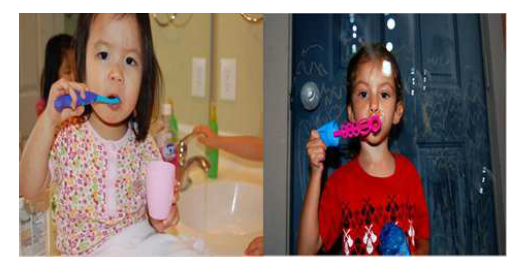
\includegraphics[width=0.7\textwidth]{similar_pose_diff}}
 	\caption{دو تصویر ژست‌های یکسان ولی فعالیت‌های متفاوت را نشان می‌دهد
 		\cite{Multi_branch_Attention_Recg_still}
 		}
 	\label{fig:similar_pose_diff}
 \end{figure}
 برای این منظور از شبکه‌های کانولوشنی (CNN) استفاده شده است تا ارتباط سنجی بین اشیاء و ژست را صورت دهند. در واقع از مفهوم مکانیزم توجه استفاده شده تا این ارتباط سنجی انجام شود. ورودی هایی که برای این شبکه در نظرگرفته شده است ترکیبی از تصویر کامل، اشیاء و اجزای بدن یا همان ژست فرد است که در نهایت از این شبکه عبور می‌کند و یک کلاس‌بندی صورت می‌گیرد.\\ 
 
\section{روش های مبتنی بر موقعیت بدنی و اشیاء}

این روش ها در این دسته بندی از اطلاعاتی که از موقعیت بدنی و اشیاء در تصویر بدست می‌آید، در تشخیص فعالیت استفاده می‌کنند. همانطور که می‌دانید استفاده از اطلاعات اشیاء در جایی که تعامل بین اشیاء و انسان در شکل‌گیری فعالیت نقش دارد، بسیار موثر است. در زیر یک سری کارهایی که توجه روی موقعیت بدنی و اشیاء داشتند اشاره می‌شود.

در سال 2019 لو لی و همکارانش %
\cite{Loss_guided_actv_attention}
در یک کار متفاوت بدون درنظرگرفتن %
\gls{BoundingBox}
 انسان یا اشیاء، از خود تصویر اطلاعات مرتبط با انسان و اشیاء را با کمک مکانیزم توجه، استخراج کرده است. آنها معتقد هستند که %
 \glspl{BoundingBox}
 در داخل خودشان علاوه بر انسان اطلاعات زائد نیز دارند.\\
دراین کار از تصویر یک سری %
\lr{Heatmap}
استخراج شده است که حین آموزش به بخش‌های کلیدی تصویر مانند انسان و اشیاء مرتبط اشاره می‌کند و یک شاخه مجزا درنظر گرفته شده که مکان قرارگیری انسان را تخمین بزند. درشاخه دیگر، از ناحیه‌های برجسته استفاده شده تا محیط و اشیاء نامرتبط نادیده گرفته شود و شبکه دراین شاخه تمرکز بیشتری روی انسان و اشیاء که می‌تواند به فعالیت مرتبط هستند،‌ داشته باشد.

در سال 2020 ونتاو ما %
\cite{Human_object_relation_action}
 از قابلیت مکانیزم توجه درداخل شبکه به شکل موثر استفاده کرده است. از آنجایی که اغلب روش ها برای یافتن ارتباط بین انسان و اشیاء نیازمند یک سری اطلاعات اضافی درمورد نحوه ارتباط انسان با اشیاء هستند،‌ این کار ازاین اطلاعات بی نیاز است. درواقع با بهره مندی از مکانیزم توجه سعی کرده است این ارتباط را شکل دهد. ماژول ارتباط‌سنج انسان-اشیاء که دراین مقاله ذکر شده است این ارتباط را تشکیل می‌دهد.
 ایده اصلی این کار از یک مقاله درمورد استفاده از یک ماژول ارتباط‌سنج درجهت شناسایی اشیاء گرفته شده است %
 \cite{Relation_network_object}
 . این شبکه از دو بخش تشکیل شده است:
\begin{enumerate}
 	\item \textbf{ساختار کلی شبکه:}
برای استخراج ویژگی از شبکه ResNet %
\cite{Resnet_article}
استفاده کرده است. همچنین از آنجایی که اطلاعات انسان و اشیاء را باهم ترکیب کرده اند،‌ به %
\gls{BoundingBox}
هایشان نیز نیاز داشته اند. البته اغلب مجموعه داده‌ها 
\glspl{BoundingBox}
 انسان را فراهم کرده اند اما برای شناسایی 
\glspl{BoundingBox}
  اشیاء از Faster R-CNN استفاده شده است.\\
روش کار به این صورت است که در ابتدا از چهار بلوک کانولوشنی برای استخراج ویژگی سطح پایین تصویر استفاده می‌شود. سپس یک RoI Pooling برای استخراج ویژگی دقیق‌تر به کمک %
\glspl{BoundingBox}
 بر روی ناحیه مورد نظر اعمال می‌شود. از این به بعد شبکه به دو شاخه تقسیم می‌شود.\\
شاخه اول مربوط به ویژگی‌ها و %
\glspl{BoundingBox}
 انسان و شاخه دوم مسیر ویژگی‌ها و %
 \glspl{BoundingBox}
  اشیاء را دربر می‌گیرد. با ورود این دوشاخه به ماژول ارتباط‌سنج،‌ وزن دهی این دو انجام می‌شود و در انتها از روی امتیازات بدست آمده کلاس‌بندی صورت می‌گیرد.
	\vspace{20pt}
 	\item \textbf{:ماژول ارتباط‌سنج انسان-اشیاء}
 هدف از طراحی این بخش بهبود خصیصه‌های فعالیت درحال انجام توسط انسان است. همچنین ویژگی‌های اشیاء مرتبط با انسان را پررنگ تر می‌کند که شبکه بتواند در جاهایی که اشیاء منجربه تفاوت در فعالیت می‌شود را تشخیص دهد. (مانند تصویر %
\ref{fig:similar_pose_diff}
 که مسواک یا حباب ساز تفاوت فعالیت را مشخص می‌کند).\\
\end{enumerate}
 البته موضوعی که اینجا درنظر گرفته نشده است،‌ ژست انسان است مخصوصا وجود اشیاء مرتبط که در تشخیص فعالیت تاثیر به سزایی دارد.
  
	در سال 2023 شوآنگ لیانگ و همکارانش %
\cite{relation_with_free_obj}
کار %
\cite{Human_object_relation_action}
را بهبود دادند. آنها به‌ جای استفاده از شبکه جدا جهت استخراج %
\gls{BoundingBox}
اشیاء، از یک ماژول در داخل ساختار شبکه استفاده کردند که کار استخراج ویژگی و شناسایی ناحیه اشیاء را انجام دهد. آنها به دو ضعف در کار قبلی اشاره کردند که دراین مقاله پوشش داده اند. یکی آموزش مدل است که نیازمند در دست داشتن ناحیه‌های اشیاء است و دیگری ارتباط بین انسان و اشیاء درداخل ماژول ارتباط‌سنج است که به طور کامل در روند آموزش این ارتباط بین انسان و اشیاء یافت نمی‌شود.\\
به همین منظور از یک ماژول جدا جهت یافتن اشیاء استفاده کردند. این مدل را طوری ساختن که در روند آموزش تنها با دراختیار داشتن برچسب نوع فعالیت مدل آموزش ببیند و پارامتر‌ها طوری به روز شوند که اشیاء مرتبط با فعالیت در هنگام تشخیص فعالیت شناسایی شوند. درواقع با این کار شبکه طوری آموزش میبیند که اشیاء با فعالیت درحال انجام درارتباط باشند.
\section{روش های مبتنی بر موقعیت بدنی و ژست}

این روش ها در این دسته بندی از اطلاعاتی که از موقعیت بدنی (کل انسان در تصویر) و ژست در تصویر بدست می‌آید، در تشخیص فعالیت استفاده می‌کنند. استفاده از این اطلاعات می‌تواند دقت کارمان را در تشخیص فعالیت بالا ببرد. کارهای گذشته نشان می‌دهد که بهرمندی از این اطلاعات نتایج مطلوبی به همراه داشته است.

در سال 2017 ژیچن ژاو و همکارانش %
\cite{Single_image_semantic_body}
از اجزای بدن که می‌تواند مفهومی در فعالیت درحال انجام داشته باشد استفاده کردند. برای مثال شخصی که درحال "ریختن آب در لیوان" است و عینک نیز زده است، توجه به سر و عینک می‌تواند شبکه را گمراه کند. درحالی که توجه اصلی فعالیت رو "ریختن آب در لیوان" است که با دست انجام می‌شود. البته این موضوع را نیز درنظر گرفته اند که حالت سر زمانی که رو به پایین است،‌ نسبت به زمانی که سربه رو به بالا است فعالیت متفاوتی را می‌تواند شکل دهد. زمانی که سر رو به بالا است احتمال انجام فعالیت "نوشیدن آب" بیشتر است.\\
این مقاله نیز از این مفهوم استفاده کرده است تا شبکه را طوری طراحی کند که تمرکز روی بخش‌های موثر بدن در انجام فعالیت باشد. برای این منظور ابتدا %
\gls{Keypoints}
بدن را استخراج کردند سپس با کمک این نقاط،‌ ناحیه های بدن را از تصویر بریده و به شبکه دادند تا در این فرآیند از این ناحیه‌ها استفاده شود.  این کار موجب می‌شود شبکه وزن دهی مناسبی به اجزای بدن،‌ درهر فعالیت داشته باشد.
 
 در سال 2020 بیشان باندری %
 \cite{Body_part_aware_multitask_act}
 یک روش چند منظوره برای تشخیص فعالیت ارائه داده است. دراین ساختار داشتن نقاط کلیدی بدن یا %
\gls{Label}
  فعالیت،‌ برای شبکه کافی است و نیازی به داشتن هردو نیست. این کار بی نیاز از داشتن %
  \gls{BoundingBox}
  انسان، اشیاء و ژست است و خود شبکه تمرکز می‌کند که این بخش ها را پیدا کند. البته لازم به ذکر است که دراینجا شبکه بیشتر روی ژست و اجزای بدن تمرکز دارد تا اشیاء.\\
  دلیل اصلی اینکه روی اشیاء تمرکز ندارند این است که اعتقاد دارند زمانی که ناحیه اجزایی که درفعالیت موثر است را مشخص می‌کنیم، اشیاءی که در ارتباط با انسان هستند نیز در این ناحیه قرار می‌گیرند. برای مثال زمانی که ناحیه "دست" مشخص می‌شود، "لیوان" نیز دراین ناحیه قرار می‌گیرد. البته ممکن است اشیاء از ناحیه مشخص شده اجزای انسان بزرگتر باشد و باعث درک غلط شبکه شود.\\
ویژگی‌های تصویر را با استفاده از شبکه %
 \lr{HRNet}
 \cite{HRNet_network}
  که یک شبکه قدرتمند در زمینه استخراج ویژگی با %
\gls{MutliResolution}
   با تمرکز بر ژست انسان است،‌ استخراج کرده است. شبکه ای که طراحی کردند از 3 شاخه تشکیل شده است:\\
  1- شاخه اول مسیر ویژگی روی کل تصویر است. دراین مسیر ویژگی کمترین وضوح استخراج شده از تصویر، مورد استفاده قرار گرفته است. \\
  2- شاخه دوم مسیر %
\gls{Analysis}
  اجزاء مهم تصویر مانند انسان و پس‌زمینه است. دراین شاخه از تمام وضوح ویژگی و همچنین از اجزای بدن استفاده می‌شود تا به نوعی مکانیزم توجه بازسازی شود. توجه اصلی اینجا روی ژست در ترکیب با کل تصویر است.\\
  3- شاخه نهایی روی اجزاء مهم بدن مانند "سر، دست، پا و..." است. این اجزاء در ترکیب با ویژگی ژست انسان یک بهبود بسیارخوب درنتیجه حاصل کرده است.
  
  در سال 2020 یانگ لی و همکارانش %
  \cite{Recognition_fusing_mutple_cue}
  یک %
\gls{UnifiedStructure}
  از مدل شبکه های کانولوشنی با توجه روی ساختار بدنی و ژست انسان در تصویر ارائه کرده اند. برای اینکه کل اجزای بدن را بررسی کنند از دو شاخه و مسیر استفاده کردند.
  \begin{enumerate}
  	\item \textbf{(\gls{BodyStructureExploration})}
  	نشانه های بدن انسان، اطلاعات ارزشمندی برای درک ساختار بدن به ما می‌دهد. ازطرفی هم، نقاط کلیدی بدن محل قرارگیری اجزای بدن در تصویر را خود دارد. از نقاط کلیدی در ساخت %
\gls{Skeleton}
  	انسان که ویژگی کلی بدن انسان را توصیف می‌کند،‌ استفاده ‌می‌شود.
 \gls{Skeleton}
  	 به نوعی نگاه %
\gls{Global}
  	به بدن انسان دارد برای این بخش مسیر %
\gls{LimbAngleDescriptor}
\lr{(LAD)}
  	 تشکیل می‌شود که این ساختار 
  	  \gls{Skeleton}
  	  را در شبکه پیاده سازی کند. همچنین مسیر %
  	 \gls{StructuralBodyParts}
  	 \lr{SBP}
  	 یک نگاه %
  	 \gls{Local}
  	 به اجزای بدن دارد تا ویژگی‌های محلی هم وارد چرخه شود. مانند بخش LAD در این مسیر نیز، از نقاط کلیدی بدن استفاده می‌شود تا نواحی با اندازه مشخص از اجزای بدن از تصویر بریده شود و به عنوان یکی از ورودی های بخش دسته‌بندی کلاس (AC) در روند کلاس‌بندی شرکت کند.\\
  	 به دلیل اینکه ممکن است اندازه شخص درتصویر متفاوت باشد باید با درنظر گرفتن ارتفاع شخص در تصویر،بخش ها بریده شود. به همین منظور از تکنیک %
  	 \gls{Thresholding}
 استفاده می‌شود.
  	\item \textbf{(\gls{ActionClassification})}
  	  با ساختار و خروجی هایی که از طریق نشانه های بدن بدست آمده،‌ کلاس بندی نهایی انجام می‌شود. برای این منظور سه شاخه درنظر گرفته می‌شود که ویژگی های بدست آمده کامل در روند تشخیص فعالیت نقش داشته باشند. هرکدام ازاین شاخه های بخش های مختلفی از تصویر را دربرمی‌گیرد.\\
 شاخه اول،‌ از کل ویژگی های بدست آمده از تصویر بهره می‌برد. شاخه دوم از اجزای بدن که از بخش SBP بدست آمده است،‌ برای کلاس بندی استفاده می‌کند و شاخه سوم به ویژگی 
  \gls{Skeleton}
  بدن که از بخش LAD محاسبه شده است توجه دارد. این سه بخش در تعامل باهم در یک روند امتیاز‌دهی شرکت می‌کنند و با ترکیب شدن امتیازات این سه بخش یک تشخیص فعالیت دقیق تری صورت می‌گیرد. 
  \end{enumerate}
در این پایان نامه نیز از این نوع نگاه به ژست، که درترکیب با موقعیت بدنی منجربه نتیجه مطلوب می‌شود استفاده شده است.
   
   	در سال 2024 ژین بیا لو و همکارانش %
   \cite{a_key_points_assisted_net}
   شبکه‌ای طراحی کردند که از دو مسیر برای استخراج ویژگی بهره می‌برد. مسیر اول اطلاعات کلی از تصویر را با شبکه عصبی کانولوشنی استخراج می‌کند. دراین مسیر از شبکه EfficientNet با اعمال تغییراتی استفاده شده است. مسیر دوم،‌ اطلاعات کمکی و اضافی را از تصویر استخراج می‌کند. این اطلاعات کمی از ژست استفاده می‌کند و در داخل ماژول طراحی شده،‌ که شامل یک سری لایه‌های کانولوشنی است ترکیب می‌شود. برای تخمین ژست نیز از OpenPose استفاده کردند.\\
   جهت افزایش کارایی شبکه از یادگیری انتقالی نیز استفاده کردند. به این صورت که یک شبکه بزرگتر انتخاب کردند و وزن‌‌های شبکه اصلی را که قرار‌ است کار تشخیص فعالیت را انجام دهد، با وزن های شبکه بزرگتر در ابتدای آموزش جایگزین شده است. 
   
   در سال 2024 پاوان و همکارش %
   \cite{shape_orbicular_grid_action}
   روی ناحیه بدن انسان تمرکز کرده و پس زمینه را حذف کردند. چون دریک فعالیت اجزای بدن انسان است که موجب می‌شود فعالیت انسانی صورت گیرد. دراین مقاله نیز روی موقعیت بدنی و ژست شخص جهت تشخیص فعالیت تمرکز کردند.\\
   ابتدا تصویر را به تصویر سطح خاکستری تبدیل کردند و با %
   \gls{Thresholding}
   ، اشیاء یا انسان را از پس زمینه جدا کردند. با استفاده از الگوریتم Canny لبه‌ها را استخراج کردند. سپس از این لبه‌‌ها به انسان و اشیاء متصل به انسان رسیدند. سپس از مرکز این تصویر یک سری بخش‌هایی را به صورت دایره‌ای وار بریدند و بادرکنارهم گذاشتن این بخش‌ها تخمینی از فعالیت انجام دادند.
   
\section{روش های مبتنی بر ژست، اشیاء و موقعیت بدنی}
روش های موجود در این دسته بندی از اطلاعاتی که از موقعیت بدنی، اشیاء و ژست در تصویر بدست می‌آید، در تشخیص فعالیت استفاده می‌کنند. تصویری که شامل فعالیت درحال انجام است هر سه این اطلاعات را دارد. البته در مواردی ممکن است اشیاء وجود نداشته باشد مانند "دویدن" ولی در اکثر مواقع اشیاء و محیط حضور دارند. با این حال مقالات زیر از این سه بخش درکار خود سود برده اند که به چند تایی از این ها می‌پردازیم.

 در سال 2018 هاو شو فانگ و همکارانش %
\cite{Pairwise_bodypart_att_2018}
به صورت خاص محور روی اعضایی از بدن که با اشیاء مرتبط با فعالیت، در تعامل هستند توجه کرده اند. در یک فعالیت مانند "نوشیدن آب" به لیوان آب و همچنین "دست" و "بازو" که لیوان را نگه داشته توجه شده است. این نوع نگرش منجر شده که از مکانیزم توجه در این کار استفاده شود. روشی که استفاده کردند از هردو اطلاعات گلوبال یا کلی و محلی بهره می‌برد. اطلاعات کلی تصویر شامل انسان، صحنه ای که فعالیت درآن درحال انجام است و اشیاء می‌شود. این نوع از ساختار باعث ترکیب هرسه این اطلاعات می‌شود و یک خروجی کلی ارزشمند از فعالیت می‌دهد.\\
برای اطلاعات محلی که ایده اصلی و پیشنهاد مقاله است،‌ از یک ماژول که به صورت جفت، اجزاء بدن را دریک مکانیزم توجه بررسی می‌کند،‌ استفاده شده است. این کار ارتباط بین ویژگی های محلی و هرجزء بدن را پیدا می‌کند. درنهایت پس از ترکیب این ویژگی ها،‌ چند تا دسته برتر انتخاب شده و در ترکیب دوباره با ویژگی های کلی،‌ وارد مرحله کلاس‌بندی می‌شود.

در سال 2021 سید سجاد اشرفی %
\cite{action_multi_att_weakly}
با توجه به اینکه فعالیت درحال انجام در یک محیطی انجام می‌گیرد، یک سری ناحیه‌های برجسته را از این محیط استخراج کرده است. ازآنجایی که هیچ مرز مشخصی در محیط برای این ناحیه‌های برجسته وجود ندارد،‌ استخراج این ناحیه‌ها با چالش هایی همراه بوده است. برای غلبه براین چالش یک روش پیشنهادی به نام شبکه هدایت شده دارای چندین مکانیزم توجه به صورت هدایت شده معرفی شده است که بتواند چندین ناحیه برجسته را همزمان تشخیص دهد.
 برای اینکه شبکه بتواند روی این ناحیه‌ها تمرکز کند، از روش معلم-دانش آموز برای تقطیع دانش بهره برده است. \\
 برخی از روش‌ها که گفته شد باتوجه به اطلاعات اضافی مانند اشیاء و ژست به شبکه در امر تشخیص فعالیت کمک می‌کنند. استفاده از این اطلاعات برای شبکه سودمند است ولی نیازمند یک سری الگوریتم‌های پیچیده برای تخمین ژست و شناسایی اشیاء است. همچنین ناحیه‌های برجسته، اطلاعاتی از ژست و اشیاء را درخودشان دارند زیرا ناحیه‌های مهمی که فعالیت درآن بخش درحال انجام است،‌ شامل ژست و اشیاء مرتبط با فعالیت نیز می‌شود.\\
 همچنین این کار روی چندین ناحیه برجسته،‌ به جای یک ناحیه توجه می‌کند. دلیلش هم این است که درفعالیتی که رخ می‌دهد،‌ ممکن است چندین شیء و یا ناحیه در شکل‌گیری این فعالیت نقش ایفا کنند بنابراین باید همه این ناحیه‌ها را در تصمیم‌گیری لحاظ کرد.\\
شناسایی چندین ناحیه برای شبکه کار مشکلی است و استفاده از یک هدایت کننده کارمعقولی است بنابراین استفاده از مکانیزم توجه دراینجا موثر بوده است. همچنین از یک شبکه معلم-دانش آموز استفاده شده که این مکانیزم توجه که درشاخه دانش آموز قرار می‌گیرد، به شکل درستی آموزش ببیند. شبکه معلم بدلیل قدرتمند بودن نسبت به شبکه دانش آموز،‌ بهترین نواحی را استخراج می‌کند که دربخش شبکه دانش آموز بسیار کمک کننده است.\\
ساختار پیشنهادی این مقاله،‌ استفاده از %
\gls{Function}
 خطاهای
کمکی در آموزش شبکه و Kmeans%
\RTLfootnote{یک الگورتیم بدون ناظر برای خوشه‌بندی می‌باشد}
برای پیداکردن یک سری نواحی برجسته برای %
\gls{BoundingBox}
 می‌باشد. تابع‌های خطا درهر بخش وظیفه‌ی خاص خود را دارند. در یک شاخه یک کمک کننده براش شناسایی اشیاء و نواحی برجسته در تصویر که در ارتباط با فعالیت است، نقش ایفا می‌کند. در شاخه دیگر ناحیه‌ای که انسان قرار دارد را تشخیص می‌دهد و در شاخه آخر به عنوان کلاس‌بند دراین ساختار حضور دارد.

در سال 2022 ژیانگتاو ژنگ و همکارانش %
\cite{Human_action_multiple_s_clue}
یک رویکردی پیشنهاد داده اند که از روی چندین نشانه از روی اطلاعات ثابت تصویر بدون نیاز به %
\glspl{BoundingBox}
 انسان و اشیاء، می‌تواند یک تشخیص مناسب انجام دهد.\\
برای تشخیص فعالیت سه عامل و نشانه در تصویر وجود دارد،‌که اغلب از این سه نشانه برای تشخیص فعالیت استفاده می‌شود:

\textbf{1- اجزاء احاطه شده:}
اجزاء احاطه شده می‌تواند شامل کل اجزاء صحنه در تصویر مانند پس زمینه‌ای که فعالیت درآن شکل گرفته است یا کل تصویر باشد.
 
 \textbf{2- اجزاء انسان:}
 اجزاء انسان می‌تواند شامل ژست یا موقعیت بدنی انسان باشد که همیشه یکی از عوامل متمایز کننده نوع فعالیت بوده است.
 
 \textbf{3- اجزاء مرتبط با فعالیت:}
می‌تواند شامل اجزاء مختلف مانند اشیاء مرتبط با انسان یا اشیاء در تعامل با فعالیت،‌ که درکنار موقعیت بدنی فعالیت درحال انجام را نشان می‌دهد، باشد. برای مثال "در دست گرفتن گوشی" در فعالیت "عکس گرفتن"  و یا "دوچرخه" در فعالیت "دوچرخه سواری". این بخش در تشخیص فعالیت بسیار موثر است.\\
این مقاله نیز مانند مقاله %
\cite{action_multi_att_weakly}
از %
\gls{BoundingBox}
 انسان و اشیاء در داخل شبکه استفاده نکرده است و باکمک مکانیزم توجه سعی می‌کند این نواحی را پیدا کند. ازاین رو رویکردی که پیشنهاده شده است از شبکه ای برای یافتن چندین نشانه فقط از روی اطلاعات موجود در تصویر استفاده ‌می‌شود. دو مسیر اصلی وجود دارد:\\
اول یک مسیر ویژگی‌های اصلی اجزای بدن انسان مانند ژست و موقعیت بدنی را استخراج می‌کند. این بخش فقط از روی برچسب اصلی فعالیت این عمل را انجام ‌می‌دهد. بعد از این ویژگی‌های بدست آمده وارد یک بخش با سه شاخه می‌شود که سه عاملی که بالا گفته شد را در تصویر تشخیص دهد. این کار نتایج مطلوبی داشته و دقت 93\% نیز بدست آمده است که نسبت به روش‌هایی که از %
\glspl{BoundingBox}
 آماده استفاده کردند کمتر است.
\section{جمع بندی فصل}

دراین فصل روش‌های ارائه شده در حوزه تشخیص فعالیت که براساس تک تصویر عمل ‌می‌کنند مورد بررسی قرار گرفتند. در حوزه تشخیص فعالیت تک تصویر سه بخش اصلی موقعیت بدنی، ژست و اشیاء نقش مهمی برای مدل جهت شناخت فعالیت درحال انجام دارد که مقاله‌های معتبر مرتبط در این بخش بررسی شدند.

مقالات مختلف زیادی دراین زمینه منتشر شده است که هرکدام به جنبه‌های از استفاده این بخش ها پرداختند با این حال دربعضی از این مقالات ژست و اشیاء نادیده گرفته شدند. در بعضی از مجموعه داده‌ها اشیاء نقش پررنگی در تشکیل آن فعالیت دارند. دراین نوع مجموعه داده‌ها مقالات مربوطه که اشیاء را نادیده می‌گیرند عملکرد به مراتب ضعیف‌تری داشته اند همچنین درمجموعه داده‌های دیگر ژست عامل اصلی شکل گیری آن فعالیت است و روش هایی که ژست را نادیده گرفته اند در این پیش بینی این فعالیت ها عملکرد ضعیفی داشتند.

بعضی موارد که از اطلاعات ازپیش‌آماده مانند ناحیه‌ی انسان و اشیاء بی‌نیاز بودند هم بررسی شدند. البته الگوریتم‌های مختلف بسیاری برای بدست آوردن این ناحیه‌ها وجود دارد که در روش پیشنهادی از این الگوریتم‌ها برای بدست آوردن این ناحیه‌ها استفاده می‌شود. درکناراین،‌ اکثر مجموعه داده‌ها در کاربرد تشخیص فعالیت،‌ اطلاعات ناحیه اشیاء و انسان را دراختیارمان قرار می‌دهند و دراین پایان نامه فقط نقاط کلیدی انسان با الگوریتم هایی بدست می‌آید.

در فصل بعد،‌ با بررسی نقاط ضعف و قوت روش‌های مختلف و همچنین استفاده از بخش‌های موثر و مفید معرفی شده، راهکار جدیدی برای ترکیب ویژگی‌های بدست آمده از تصویر در جهت تشخیص فعالیت انسان معرفی خواهد شد.
		% فصول دوم: مروری بر مطالعات انجام شده
% !TeX root=../main.tex
\chapter{روش پیشنهادی}
%\thispagestyle{empty} 
\section{مقدمه} 

در این بخش قسمت های مختلف الگوریتم پیشنهادی برای تشخیص نوع فعالیت انسان در تک تصویر بررسی می‌شود. برای درک نوع فعالیت درحال انجام، عوامل مختلفی می‌توانند دخیل ‌باشند. ازجمله طرز ایستادن شخص که ژست انسان را نشان می‌دهد،‌ صحنه‌ای که فعالیت درآن درحال انجام است مثل زمین تینس در بازی تنیس و یا اشیاء که انسان با آن تعامل دارد مثل "لیوان" در فعالیت "نوشیدن آب".\\
روش پیشنهادی از چندین مرحله تشکیل می‌شود که درادامه به تفصیل بررسی می‌شود. ترکیب ژست با موقعیت بدنی داخل یک مکانیزم توجه از جمله مهم ترین مراحل بشمار می‌رود و چالش‌های زیادی مانند تخمین ژست در حالت های مختلف انسان،‌ به‌دست آوردن ناحیه های کلیدی،‌ %
\gls{Occlusion}
بعضی اجزاء بدن و عوامل گمراه کننده برای شبکه وجود دارد.\\
روش ها و الگوریتم‌های مختلفی برای تشخص فعالیت در تک تصویر وجود دارد. روش‌های مبتنی بر موقعیت بدنی و ژست، موقعیت بدنی و اشیاء، اشیاء و ژست و روش ترکیبی موقعیت بدنی، ژست و اشیاء که جزء بهترین روش‌‌ها بشمار می‌رود و اغلب به نتایج امیداورکننده رسیده است. هرکدام از این روش‌‌ها و الگوریتم‌ها دارای مزایا و معایبی هستند که هرکاربرد خاصی باید الگوریتم تشخیص حرکت مناسبی را درنظر گرفت.\\
با درنظر گرفتن چالش‌های موجود در کاربرد مورد نظر و نقاط ضعف و قوت روش‌های موجود از موقعیت بدنی،‌ اشیاء و ژست برای تشخیص فعالیت در تک تصویر استفاده شده است. برای ترکیب ویژگی‌های ظاهری انسان که موقعیت بدنی را نشان می‌دهد با ژست از مکانیزم توجه استفاده شده است. همچنین دراین فصل درباره نحوه محاسبه یک بردار ویژگی برای ژست انسان در یک روش بدون مکانیزم توجه برای مقایسه با مکانیزم توجه بحث شده است.

\section{مراحل الگوریتم پیشنهادی}

\begin{figure}[ht]
	\centerline{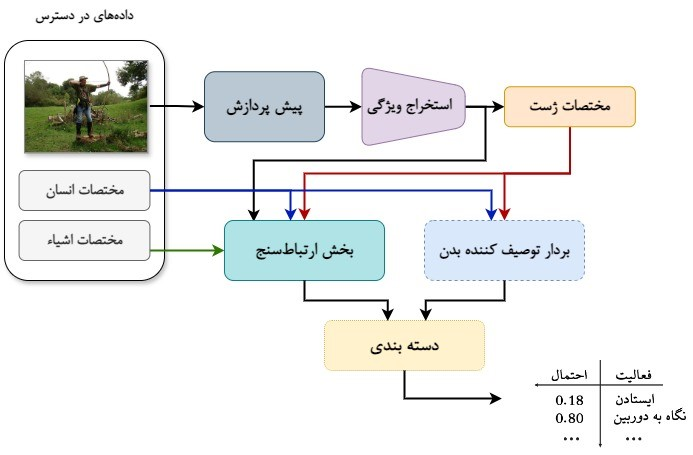
\includegraphics[width=0.8\textwidth]{Flowchart_whole}}
	\caption{
	\hl{ساختار کلی شبکه پیشنهادی}
	}
	\label{fig:Flowchart_whole}
\end{figure}
شکل %
\ref{fig:Flowchart_whole}
ساختار کلی طراحی شده را نشان می‌دهد. از یک بخش ارتباط‌سنج %
\gls{RelationModule}
برای ترکیب ویژگی‌های انسان با اشیاء که شبکه ResNet کار استخراج ویژگی را انجام می‌دهد،‌ استفاده شده است. 
پس از انجام پیش‌ پردازش‌های لازم جهت بهبود کیفیت تصویر، غلبه بر مشکلات انسداد، نرمال سازی و تقویت داده‌ها، نواحی مهم از جمله ناحیه انسان، اشیاء و اجزاء بدن از تصویر بریده می‌شود و ویژگی های آنها از یک شبکه عصبی عمیق استخراج می‌شود. همچنین برخی تغییرات در رنگ و اندازه تصویر داده می‌شود تا داده‌ها تنوع بیشتری به خود بگیرند که این تغییر رنگ و اندازه یک سری چالش‌هایی نیز دارد که در بخش %
\ref{pishe_pishnehadi}
بیشتر توضیح داده می‌شود.
از ویژگی‌های استخراج شده جهت تخمین مختصات ژست استفاده می‌شود و سپس این مختصات در کنار مختصات انسان و اشیاء در بخش‌های بعدی استفاده می‌شود. همانطور که در شکل %
\ref{fig:Flowchart_whole}
نشان داده شده، بخش ارتباط‌سنج از سه مختصات موقعیت بدنی انسان، اشیاء و ژست استفاده می‌کند که یک خروجی معنادار و ارتباط‌ یافته تولید کند. مسیر بردار توصیف کننده بدن، یک روش پیشنهادی دراین پایان نامه است که از مختصات ژست و موقعیت بدنی استفاده می‌کند که یک بردار از ژست تشکیل دهد. در ادامه خروجی این دو بخش باهم ترکیب شده و یک دسته‌بندی انجام می‌شود.
البته درون بخش ارتباط‌سنج یک نوعی ژست با موقعیت بدنی ‌انجام می‌شود که به عنوان بخش اضافی بررسی می‌شود.

\subsection{مرحله پیش پردازش}\label{pishe_pishnehadi}

در این مرحله باید ابتدا کانال تصویر رنگی از هرکانالی که است به RGB تغییر پیدا کند. اصولاً شبکه‌های عصبی با این ساختار بهتر به نتیجه می‌رسند. تصاویر موجود اغلب کیفیت مناسبی دارند بااین حال برخی از تصاویر وضوح بسیار پایینی دارند که شناسایی شخص دراین تصویر حتی برای انسان نیز کار دشواری است. این تصاویر از فهرست داده ها حذف شده است.
در ادامه مراحل پیش پردازش در چند بخش مورد بررسی قرار گرفته است:
\subsubsection{نرمال سازی داده}

یکی از ابعاد اساسی در پیش‌پردازش تصاویر، نرمال‌سازی است که بهبود قابلیت‌ها و عملکرد مدل‌ها را تضمین می‌کند. تصاویری که به صورت ورودی به مدل‌های یادگیری عمیق و الگوریتم‌های تصویری داده می‌شوند، معمولاً شامل متغیرهایی مانند روشنایی، کنتراست، و زاویه‌های مختلف هستند. این تغییرات متنوع و گاهی پیچیده در تصاویر می‌توانند باعث مشکلات در یادگیری مدل‌ها شوند. بنابراین، نیاز به یک مرحله پیش‌پردازش قوی و موثر که تصاویر را به یک وضعیت استاندارد و قابل تشخیص تبدیل کند، اساسی است.

نرمال‌سازی تصاویر یکی از اصول اساسی در پیش‌پردازش است که بهبودی در تطبیق مدل با داده‌ها و افزایش قابلیت تعمیم مدل به داده‌های جدید را ایجاد می‌کند. این مرحله اقدام به تعیین وضعیت استاندارد برای تصاویر دارد تا مدل بتواند با ورودی‌های متفاوت و شرایط مختلف بهتر سازگار شود.

شکل %
\ref{fig:normalization_no_norm}
یک نمونه از روند یادگیری شبکه عصبی با ساختار داده‌های نرمال‌ شده و نرمال نشده را نشان می‌دهد. داده‌های نرمال نشده حرکت‌های زیگزاگی را در طی آموزش دارند و برای رسیدن به جواب بهینه تعداد گام‌های بیشتری را طی می‌کنند درحالی که داده‌های نرمال شده شکل حرکتی منظم‌تری دارند. طول این محور با پارامتر %
\gls{LearningRate}
مشخص می‌شود. بنابراین در داده‌های نرمال نشده نرخ یادگیری بزرگتری نیاز است تا مدل مسیر اولیه خود را پیدا کند و در گام‌های بعدی نرخ یادگیری ها متفاوت می‌شود درحالی که در داده نرمال شده،‌ باید یک نرخ یادگیری ثابت به جواب بهینه دست پیدا می‌کند.

\begin{figure}[ht]
	\centerline{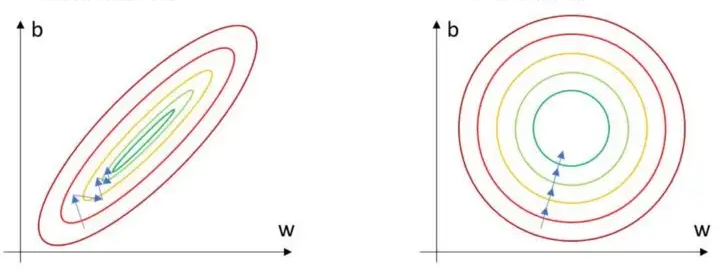
\includegraphics[width=0.8\textwidth]{normalization_no_norm}}
	\caption{\hl{
		فرآیند یادگیری شبکه عصبی با داده نرمال شده (راست) و داده نرمال نشده (چپ)
		}
	 \cite{Normal_not_Normal}
	}
	\label{fig:normalization_no_norm}
\end{figure}

در ادامه توضیحات، به بررسی روش‌های مختلف نرمال‌سازی تصاویر پرداخته و سپس به بررسی یکی از روش‌های مفید‌ترین نرمال‌سازی، یعنی  نرمال‌سازی میانگین و واریانس، پرداخته خواهد شد. استفاده از  نرمال‌سازی میانگین و واریانس به عنوان یک روش مؤثر در نرمال‌سازی تصاویر در شبکه‌های عصبی اهمیت بیشتری یافته است و به بهبود سرعت و عملکرد آموزش مدل‌ها کمک زیادی می‌کند. همچنین درداخل شبکه از %
\gls{BatchNormalization}
 نیز جهت نرمال‌سازی استفاده شده است که ادامه بررسی می‌شود.
\begin{itemize}
	\item \textbf{نرمال سازی به روش :Min-Max }
	در این روش، مقادیر پیکسل‌ها به گونه‌ای تغییر می‌کنند که حداقل مقدار به صفر و حداکثر مقدار به یک تبدیل شوند. این نرمال‌سازی معمولاً برای تصاویری با دینامیک مقادیر محدود مفید است.
	\item \textbf{نرمال سازی به روش :Z-Score }
	 این روش تصویر را به نحوی نرمال‌سازی می‌کند که میانگین آن صفر و انحراف معیاری به یک تغییر یابد. این نرمال‌سازی اغلب برای تصاویری با توزیع‌های پیچیده استفاده می‌شود.
\end{itemize}
دو روش که در بالا گفته شد، یک سری معایبی دارند از جمله روی داده ها با توزیع گسترده و انحراف معیار‌های بزرگ عملکرد ضعیفی دارند همچنین در تصاویر با توزیع های غیر معمول چندان کارایی مطلوبی ندارند. دو روش نرمال‌سازی استفاده شده در زیر توضیح داده می‌شود.

$\bullet$ \textbf{نرمال‌سازی میانگین و واریانس}
\LTRfootnote{Mean and  Variance Normalization}
:\\
در این روش، میانگین تمام پیکسل‌ها از تصویر کم می‌شود تا میانگین آن به صفر برسد. سپس واریانس نیز تا یک مقداری تغییر می‌کند. این کار به مدل کمک می‌کند تا با داده‌هایی که به صورت معیارهای نرمال سازی شده هماهنگ شود.

طبق فرمول 
 \ref{eq:normalizaion}
داده‌های نرمال‌ شده از تفریق میانگین %
$\mu$
 از داده‌ها و تقسیم شدن بر انحراف معیار %
 $\sigma$ 
 به دست می‌آید.
\begin{equation}
	\label{eq:normalizaion}
	x:=\frac{x-\mu}{\sigma}
\end{equation}

انحراف معیار در اینجا از فرمول %
\ref{eq:enheraf_meyar}
 بدست می‌آید که %
 $E[X]$
  میانگین را نشان می‌دهد.
  \begin{equation}
  	\label{eq:enheraf_meyar}
  	  \sigma=\sqrt{E\left[X^2\right]-(E[X])^2}
  \end{equation}
  
$\bullet$ \textbf{نرمال‌سازی دسته‌ای در ساختار شبکه عصبی}
:\\
در شبکه‌های عصبی، از نرمال سازی دسته‌ای به عنوان یک لایه نرمال‌سازی استفاده می‌شود. این لایه برای هر دسته از داده‌ها، میانگین و انحراف معیار محاسبه کرده و مقادیر ورودی را مطابق با آنها نرمال‌سازی می‌کند. 
استفاده از نرمال‌سازی دسته‌ای به عنوان یک روش مفید در نرمال‌سازی تصاویر به ویژه در شبکه‌های عصبی توصیه می‌شود. این روش نه تنها باعث نرمال‌سازی میانگین و انحراف معیار است، بلکه به شبکه عصبی کمک می‌کند تا سریع‌تر و بهتر آموزش ببیند. نرمال‌سازی دسته‌ای همچنین مشکل %
\gls{VanishingGradients}
 را کاهش می‌دهد و از مشکل برخورد با مشکل %
\gls{ExplodingGradients}
 جلوگیری می‌کند. این روش بهبود قابل توجهی در سرعت و کارایی یادگیری شبکه‌های عصبی دارد و بنابراین در بسیاری از حوزه‌های بینایی ماشین مورد استفاده قرار می‌گیرد.
 
  \subsubsection{افزایش داده}
 در حوزه یادگیری عمیق و تشخیص فعالیت‌ها در تصاویر، پیش‌پردازش تصاویر با %
 \gls{DataAugmentation}
 یکی از مراحل حیاتی است که تاثیر قابل توجهی بر عملکرد مدل‌های یادگیری عمیق دارد. با توجه به محدودیت داده در بسیاری از موارد، افزایش داده به عنوان یک روش مؤثر و اساسی در بهبود دقت و قابلیت تعمیم مدل‌ها به مسائل واقعی و متنوع مورد استفاده قرار می‌گیرد.
 
 توسعه تکنولوژی و افزایش استفاده از شبکه‌های عصبی عمیق، نیاز به داده‌های بزرگ‌تر و متنوع‌تر را ایجاب کرده است. هرچند ممکن است در بعضی از حوزه‌ها داده‌های زیادی در دسترس باشد، اما در حوزه تشخیص فعالیت‌ها، اغلب با محدودیت داده مواجه هستیم. این مسئله می‌تواند منجر به بروز مشکلاتی مانند بیش‌برازش یا کم‌دادگانی شود که در نهایت باعث کاهش دقت و قابلیت تعمیم مدل می‌شود.

 \textbf{اهمیت افزایش داده:}

 با توجه به محدودیت داده در بسیاری از حوزه‌ها، افزایش داده به عنوان رویکردی مؤثر در جلوگیری از بروز مشکلاتی مانند %
\gls{Overfitting}
  یا کم‌دادگانی به شمار می‌آید. این روش از طریق تولید نمونه‌های جدید از داده‌های موجود، مدل را به موارد مختلف و ناشناخته مواجه می‌کند و این امکان را فراهم می‌کند که مدل در شرایط مختلف عملکرد مناسبی از خود نشان دهد. افزایش داده به ویژه در مواردی که داده محدود است، کمک می‌کند تا مدل به طور کلی عملکرد بهتری داشته باشد. در ادامه، به بررسی مراحل و تکنیک‌های پرکاربرد در افزایش داده و نیز ارائه راهکارهایی برای اجرای بهینه این عملیات می‌پردازیم.\\
  
 \textbf{\hl{در فرآیند افزایش داده ملاحظات زیر درنظر گرفته می‌شود:}}
\begin{itemize}
	\item \textbf{تطبیق با خصوصیات مسئله:}
	تکنیک‌های افزایش داده باید خصوصیات مسئله و نوع داده را درنظر بگیرند. مثلاً در تشخیص فعالیت‌ها، چرخش تصویر ممکن است برای تصاویر فعالیت انسانی مناسب‌تر باشد.
	
	\item \textbf{پیش‌پردازش همراه با افزایش داده:}
	برخی از تکنیک‌های پیش‌پردازش مانند نرمال‌سازی تصویر می‌توانند با افزایش داده ترکیب شوند و به بهبود تعمیم مدل کمک کنند.
	
	\item \textbf{ارزیابی اثربخشی تغییرات:}
	ارزیابی دقیق تأثیر هر تغییر در دقت و عملکرد مدل ضروری است تا تصمیمات بهینه‌تر در انتخاب تکنیک‌ها گرفته شود.
	
	\item \textbf{استفاده از چند تکنیک به صورت ترکیبی:}
	استفاده از ترکیب چند تکنیک افزایش داده می‌تواند به تنوع بیشتر و بهبود قابلیت تعمیم مدل منجر شود.
\end{itemize}

چند نوع افزایش داده یا تغییرات داده انجام شده که درزیر به آنها اشاره می‌شود:

\textbf{1. \gls{Rotation}}
\textbf{:}
تصویر با زاویه‌های تصادفی چرخش داده می‌شود. این کار به مدل کمک می‌کند تا اجسام از هر زاویه‌ای تشخیص داده شوند.

\textbf{2. \gls{Scaling}}
\textbf{:}
تصویر به اندازه‌های تصادفی کوچکتر یا بزرگتر شده و سپس به اندازه مورد نظر برگردانده می‌شود. این تغییرات موجب بهبود تعمیم‌پذیری مدل می‌شود.

\textbf{3.  \gls{HVFlip}}
\textbf{:}
تصویر به صورت افقی یا عمودی بازانعکاس داده می‌شود. این تغییرات باعث افزایش تنوع داده و تشخیص صحیح‌تر اجسام می‌شود.

\textbf{4.  \gls{ColorJittering}}
\textbf{:}
اعمال تغییرات تصادفی در رنگ‌های تصویر مانند تغییر روشنایی، کنتراست و اشباع. این کار به مدل کمک می‌کند تا با تنوع بیشتری در برابر تغییرات نوری مقاوم باشد.

انجام برخی از این تغییرات روی تصویر ممکن است منجبر به یک سری خطاهای دیگر شود. تغییراتی مانند چرخش و تغییر اندازه باعث می‌شود %
\glspl{BoundingBox}
که برای اشیاء و انسان دردسترس است با خطا مواجه شود. برای غلبه براین مشکل باید تغییراتی که باعث می‌شود اندازه تصویر تغییرات کند روی %
\glspl{BoundingBox}
 موجود نیز اعمال شود. 

دو نمونه از تصاویر بدون اعمال تغییرات و با اعمال تغییرات به ترتیب در شکل %
 \ref{fig:no_album}
 و
\ref{fig:with_album}
نشان داده شده است.
\begin{figure}[ht]
	\centerline{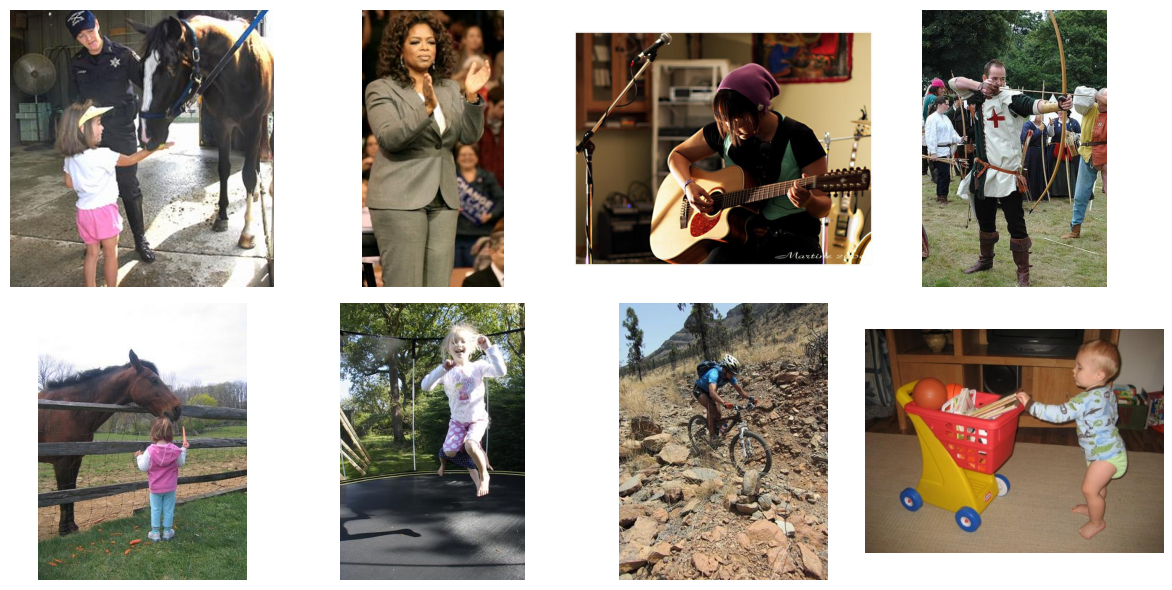
\includegraphics[width=0.8\textwidth]{no_album}}
	\caption{تصاویر بدون اعمال تغییرات}
	\label{fig:no_album}
\end{figure}
\begin{figure}[ht]
	\centerline{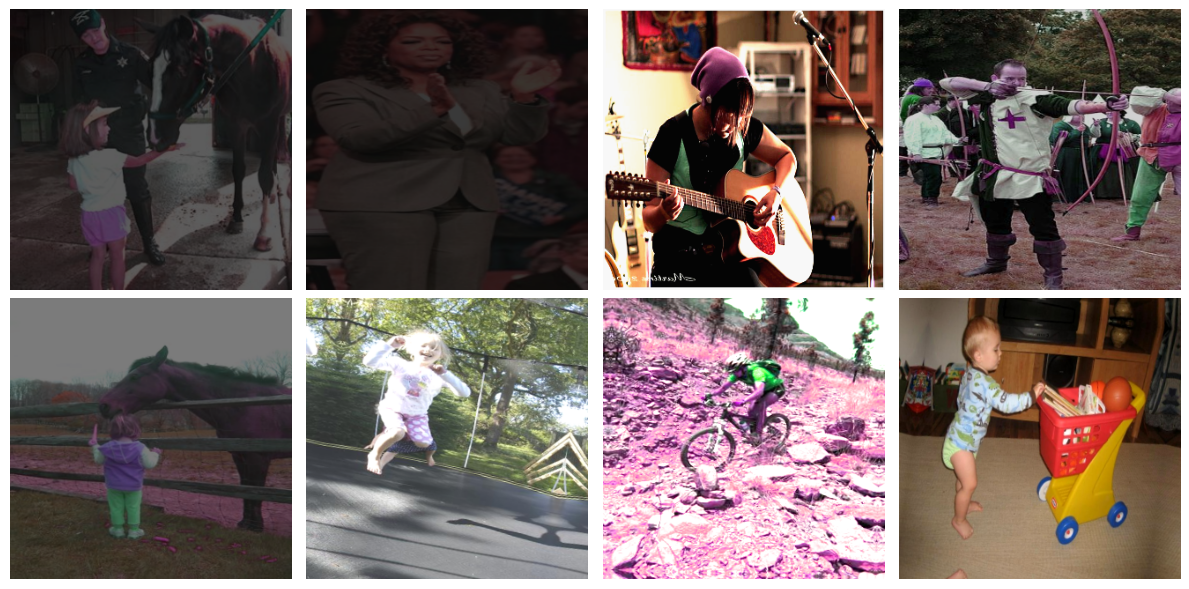
\includegraphics[width=0.8\textwidth]{with_album}}
	\caption{تصاویر با اعمال چندین نوع تغییرات}
	\label{fig:with_album}
\end{figure}
همانطور که مشخص است اندازه تمامی تصاویر به یک اندازه مشخص درآمده است و هدف از اینکه اندازه تمامی تصاویر یکسان است این است که شبکه نمی‌تواند اندازه‌های مختلف را اداره کند و نیاز است که اندازه تمامی تصاویر باهم برابر باشد. همچنین روی تمامی تصاویر چندین نوع تغییرات شامل چرخش، تغییر اندازه، انعکاس و تغییر رنگ با درصد احتمال‌های متفاوت اعمال شده است.البته اینطور نیست که اگر تصویری تغییر رنگ داشته دیگر چرخش نداشته باشد. ممکن است همه تغییرات اعمال شود یا برعکس هیچ تغییری نداشته باشد.

\subsection{تخمین نقاط کلیدی بدن یا ژست}

در زمینه تشخیص فعالیت انسان، تخمین نقاط کلیدی بدن اهمیت بیشتری پیدا می‌کند. این حوزه در بسیاری از کاربردها از جمله نظارت امنیتی، تحلیل حرکت، تشخیص بیماری‌های عضلانی، و حتی سیستم‌های واقعیت افزوده استفاده می‌شود. با توجه به تنوع و پیچیدگی فعالیت‌های انسانی، تخمین نقاط کلیدی بدن با دقت بالا و توانایی تعمیم به صحنه‌های گوناگون، یک چالش اساسی در این حوزه محسوب می‌شود.

در یک تک تصویر، تخمین نقاط کلیدی بدن به دقت و کارآیی مطلوبی نیاز دارد. این کار با توجه به وجود چالش‌های نظیر تغییرات نوری، اختلافات در اندازه افراد، و تغییرات در زوایا و جهات دید، موقعیت نقاط کلیدی بدن انسان را مورد تخمین قرار می‌دهد. این اطلاعات می‌تواند برای تفسیر و تحلیل فعالیت انسان در یک فرآیند خاص یا شرایط محیطی مفید باشد.

در این پایان نامه، از مدل YOLO%
\LTRfootnote{You Only Look Once}
 برای تخمین نقاط کلیدی بدن از تصاویر در بخش ارتباط‌سنج استفاده شده است. YOLO یک مدل شناخته ‌شده در زمینه تشخیص اجسام است که به دلیل ساختار منحصر به فرد خود به سرعت و دقت بالا معروف است. نسخه‌های دیگری نیز از این شبکه وجود دارد که روی داده‌های انسان آموزش دیده و توانایی تخمین ژست و نقاط کلیدی بدن را دارد.

استفاده از مدل YOLO نه تنها این امکان را فراهم می‌کند که به فرایند تشخیص فعالیت انسان در تصویر با سرعت انجام شود، بلکه به دلیل قابلیت تعمیم بالا، در مقابل تغییرات ناگهانی در محیط یا حرکات انسان از پایداری خوبی برخوردار است. انتخاب این مدل با توجه به نیازهای ساختار سبکه و تعامل آسان با آن، بهبود قابلیت‌ها و دقت در تخمین نقاط کلیدی بدن را فراهم می‌کند.

البته YOLO روی برخی از تصاویر عملکرد ضعیفی دارد زیرا مختصات برخی از نقاط که دچار انسداد شده‌اند را کاملاً گم می‌کند. به همین جهت از مدل MMPose در بخش توصیف کننده زاویه بدن استفاده شده است. این مدل در بعضی از نقاط دارای انسداد، یک تخمین نسبتاً درستی از نقطه کلیدی می‌دهد. در بخش مسیرتوصیف کننده بدن دانستن مختصات تخمینی نقاط کلیدی بدن بسیار موثر است زیرا باید برداری طبق این‌ مختصات محاسبه شود و با دردست نداشتن این مختصات، حتی مختصات نزدیک به نقطه واقعی افت دقت ناشی خواهد شد.

\gls{BoundingBox}
 یا مختصات ناحیه انسان و اشیاء به صورت پیش‌فرض دردسترس است. این مختصات کمک کرده تا بتوان ناحیه شخص را از تصویر و پس زمینه جدا کرد و به صورت جداگانه به مدل تخمین ژست داد تا این نقاط کلیدی را تخمین بزند. تصویر %
\ref{fig:koli_ensan_nogte}
فعالیت شخص را نشان می‌دهد که ناحیه شخص از تصویر جدا شده و درنهایت در فرآیند تخمین ژست،‌ این نقاط کلیدی تخمین زده شده است. 
  \begin{figure}
 	\centering
 	\subfloat[تصویر کامل]{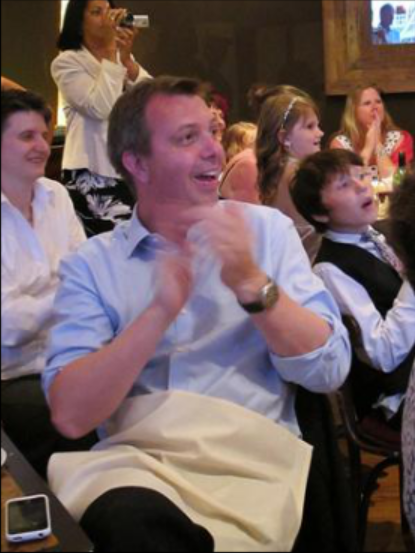
\includegraphics[width=0.24\textwidth]{ensan_salem}\label{fig:ensan_salem}}
 	\hfill
 	\subfloat[بخش بریده شده انسان]{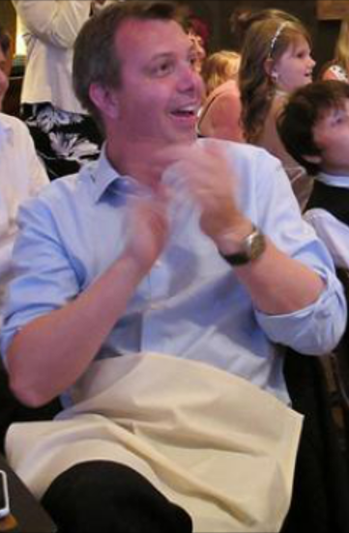
\includegraphics[width=0.22\textwidth]{ensan_boride}\label{fig:ensan_boride}}
 	\hfill
 	\subfloat[نقاط کلیدی بدن انسان]{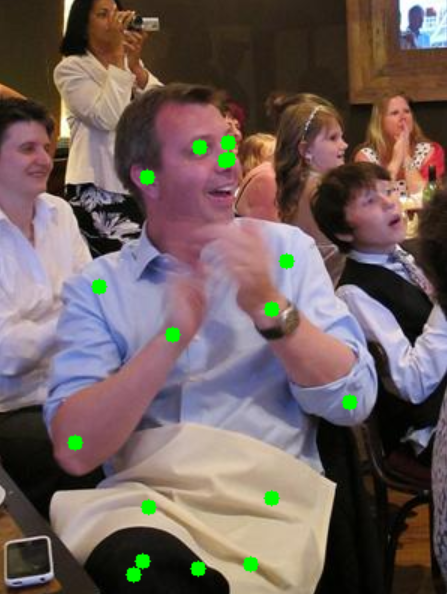
\includegraphics[width=0.24\textwidth]{ensan_nogat}\label{fig:ensan_nogat}}
 	\caption{روند کلی بدست آوردن نقاط کلیدی بدن}
 	\label{fig:koli_ensan_nogte}
 \end{figure}
 به کمک این نقاط کلیدی، %
 \glspl{BoundingBox}
  اجزای بدن ساخته می‌شود. جدول %
 \ref{tab:jadval_nahiye}
 استفاده از نقاط کلیدی مختلف را در راستای ساخت اجزاء بدن نشان می‌دهد.\\
 
  \begin{table}[ht]
 	\centering
 	\onehalfspacing
 	\arrayrulecolor{black}
 	\begin{tabular}{ l | c}
 		\rowcolor{gray}
 		\mrh{نقاط کلیدی}  & \mrh{ناحیه محاسبه شده}     \\
 		\rowcolor{gray!10} مچ دست، آرنج & مچ دست \\
 		\hline شانه، آرنج و مچ دست & آرنج \\
 		\hline
 		\rowcolor{gray!10} مچ پا، زانو & پا \\
 		\hline لگن، زانو و مچ پا & زانو \\
 	\end{tabular}
 	\caption{محاسبه نواحی بدن}
 	\label{tab:jadval_nahiye}
 \end{table}
دربرخی از تصاویر ممکن است بخشی از اجزاء بدن دچار انسداد شده باشد. به جای این بخش‌ها می‌توان فقط صفحه سفید به شبکه ارسال کرد اما در این حالت شبکه دقت پایینی را در هنگام استفاده از آن ثبت می‌کند. بنابراین برای حل این مشکل، ناحیه‌ای که انسان درآن قرار دارد به 9 بخش تقسیم می‌شود و یک بخش از آن به صورت انتخابی از بین این بخش‌ها انتخاب شده و به جای آن قسمت انسداد شده در شبکه حضور پیدا می‌کند.

همچنین مواقعی پیش می‌آید که فقط یکی از نقاط کلیدی مانند "زانو" را دراختیار داریم و فقط با داشتن یک نقاط کلیدی نمی‌توان ناحیه‌ای رسم کرد بدون اینکه فاصله زانو تا مچ پا را درنظر نگیرد، بنابراین دراین حالت‌ها با یک ضریب ثابت و درنظر گرفتن طول %
\gls{BoundingBox}
 انسان در تصویر، اقدام به محاسبه ناحیه مدنظر گرفته شده است.
  \begin{figure}
	\centering
	\subfloat[ ]{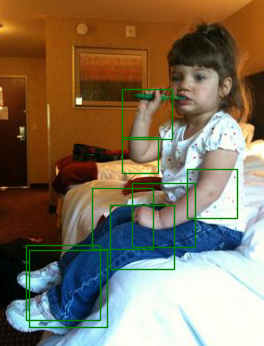
\includegraphics[width=0.22\textwidth]{keypoint_boxes1}\label{fig:keypoint_boxes1}}
	\hfill
	\subfloat[ ]{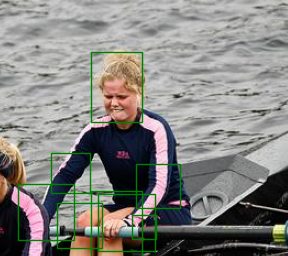
\includegraphics[width=0.28\textwidth]{keypoint_boxes2}\label{fig:keypoint_boxes2}}
	\hfill
	\subfloat[ ]{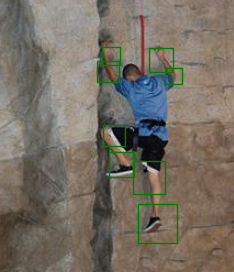
\includegraphics[width=0.22\textwidth]{keypoint_boxes3}\label{fig:keypoint_boxes3}}
	\caption{تصاویر 
		\gls{BoundingBox}
		 ژست بدست آمده از نقاط کلیدی}
	\label{fig:keypoint_boxes}
\end{figure}

در محاسبه ناحیه‌های، ناحیه "بدن" و "سر" درنظر نگرفته شده است، به این دلیل که ناحیه بدن اطلاعات خاصی را به شبکه اضافه نمی‌کند همچنین ناحیه سر نیز چندان در تشخیص فعالیت تاثیرگذار نیست.

شاید سوال باشد که در تصویر %
\ref{fig:keypoint_boxes2}
 ناحیه "سر" انتخاب شده ولی این ناحیه به جای ناحیه پا که دچار اسنداد شده به صورت جایگزین انتخاب شده است، زیرا همانطور که گفتیم یک ناحیه از انسان به صورت شانسی انتخاب خواهد شد و دراینجا سر انتخاب شده است
 
 \subsection{تعامل ژست در مکانیزم توجه}

مکانیزم توجه امکان اختصاص وزن‌های مختلف به نقاط مختلف تصویر را فراهم کرده و به شبکه‌های عصبی اجازه می‌دهد تا به نقاط مهم و حیاتی تصویر با دقت بیشتری توجه کنند. طبق این موضوع، شبکه سعی می‌‌کند ارتباط بین انسان و اشیاء که در فعالیت دخیل هستند پیدا کند. دربیشتر روش‌های تشخیص فعالیت انسان، ژست کمترین اهمیت را داشته و اصولاً این ویژگی مهم را درنظر گرفته نشده است. 
 
 \subsection{بخش اول: مسیر توصیف کننده زاویه بدن }
 
 در این بخش با استفاده از توصیف کننده زاویه بدن،‌ یک برداری بدست می‌آید که خاصیت کامل ژست انسان را توصیف می‌کند. این بردار درترکیب با خروجی بخش ارتباط‌سنج انسان و اشیاء، جهت امتیاز‌دهی و کلاس بندی استفاده می‌شود.
 
 توصیف کننده زاویه بدن، یک اسکلت از ساختار بدن انسان را تشکیل می‌دهد و اطلاعات جامع از بدن انسان استخراج می‌کند. این کار ویژگی‌های مفهومی %
\gls{High-Level}
  از تصویر را فاش ‌می‌کند و درمواقعی که ممکن است انسداد یا پوشیدگی توسط لباس باعث شود قسمتی از بدن از دسترس خارج شود، کاربرد دارد و عملکرد مدل را بهبود می‌بخشد. 
  
برای ساخت بردار ویژگی از اسکلت، اول از نقاط کلیدی که از شبکه MMPose بدست آمده، استفاده شده است. 13 نقطه کلیدی از بدن انتخاب شده است تا در ساخت بردار حرکتی بدن استفاده شود. با این نقاط یک مجموعه از بردارهای جهت‌دار بدن 
 $\left\{\mathbf{v}_l\right\}_{l=1}^L$
 ساخته شده است،‌ که در اینجا 
 .$\mathbf{v}_l \in \mathbb{R}^2$
 و L به تعداد اعضای بدن اشاره دارند.
 
 \begin{figure}[ht]
 	\centerline{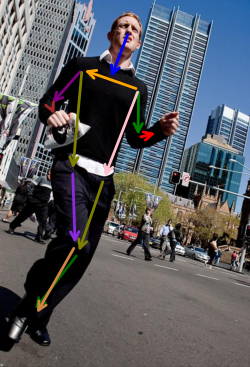
\includegraphics[width=0.28\textwidth]{limb_angle}}
 	\caption{یک نمونه توصیف کننده زاویه بدن}
 	\label{fig:limb_angle}
 \end{figure}

 همانطور که در تصویر %
 \ref{fig:limb_angle}
 مشاهده می‌کنید،‌ 12 بردار شامل 
 \textit{بالا تنه، }
 \textit{شانه، }
\textit{بازو، }
\textit{ساعد، }
\textit{بدن، }
\textit{ران پا و }
\textit{ساق پا}
می‌باشد. جهت این بردارها به کمک دو جفت نقطه کلیدی تعیین شده است.
 طبق فرمول %
 \ref{eq:angle_limb}
 بردار %
 $\mathbf{x}_l^1$
  و بردار %
   $\mathbf{x}_l^2$
 دو تا بردار نشان دهنده یک عضو هستند که با کمک این فرمول بردار جهت‌دار آن بدست آمده است.
\begin{equation}
	\label{eq:angle_limb}
	\mathbf{v}_l=\frac{\left(\mathbf{x}_l^2-\mathbf{x}_l^1\right)}{\left\|\mathbf{x}_l^2-\mathbf{x}_l^1\right\|_2}
\end{equation}

همچنین زاویه بین بردار نشان‌دهنده دو عضو بدن %
   $\mathbf{v}_{l_1}$
   و 
    $\mathbf{v}_{l_2}$
 ، از فرمول %
\ref{eq:angle_bet_limb}
  بدست آمده است.
  \begin{equation}
  	\label{eq:angle_bet_limb}
  	a_{l_1, l_2}=\mathbf{v}_{l_1}^T \cdot \mathbf{v}_{l_2}
  \end{equation}
 \hl{ در این فرمول ضرب داخلی جفت بردارهای عضو بدن محاسبه شده است، ازاین‌رو از ترکیب جفت تمامی}
  13 نقطه کلیدی باهم یک بردار به طول 78 تولید شده است (%
  $C_{13}^2=78$
  ). از روی این بردار یک بردار عضو بدن بهینه محاسبه شده است که از ترکیب جفت تمامی 78 تایی بردار با یکدیگر است که درنهایت باعث ساخت یک بردار ویژگی توصیف کننده بدن بهینه به طول 3003 شده است که ویژگی‌های بیشتر و بهینه‌تری از ژست را توصیف می‌کند(
    $C_{78}^2=3003$
  ). این ویژگی بهینه می‌تواند نیاز مدل را به حد کافی برآورده کند. %
  \cite{Recognition_fusing_mutple_cue}
  
  بردار ساخته شده درآخر با خروجی بخش ارتباط‌سنج انسان و اشیاء ترکیب شده و وارد بخش نهایی برای امتیاز‌دهی می‌شود و تعیین می‌گردد که به کدام فعالیت تعلق دارد.
  
   \subsection{بخش دوم: مسیر ارتباط‌سنج انسان و ژست}
   
 ابتدا باید تشخیص داده شود که کدام ویژگی باید با ژست ترکیب شود؟ آیا ترکیب ویژگی‌های اشیاء با ژست نتیجه بهتری می‌دهد یا موقعیت بدنی با ژست؟ در جواب باید گفت که ترکیب ویژگی‌های موقعیت بدنی انسان با ژست انتخاب معقول‌تری است. زیرا ارتباط بین اشیاء و ژست حتی برای انسان نیز چندان واضح نیست. علاوه‌ بر این در ارتباط بین موقعیت بدنی و اشیاء، این ارتباط تا حد زیادی شکل گرفته است و اضافه کردن این ارتباط فقط حجم محاسبات در شبکه را زیاد خواهد کرد و باعث افزایش اطلاعات زائد می‌شود. از این رو دراین پژوهش انتخاب ما ترکیب با موقعیت بدنی است.
 
  ترکیب ویژگی‌های موقعیت بدنی انسان با ژست کمک می‌کند که آن دسته از فعالیت‌هایی که بیشتر با ژست درگیر هستند می‌آید، درآنها اعضای بدن در یک نوع دید محلی درشبکه درنظرگرفته شوند و درنهایت توصیف بهتری از فعالیت درحال انجام به ثمر برسد.
 
 با کمک مکانیزم توجه یکسری ویژگی‌های معنادار و مرتبط بین اجزای ورودی یافت می‌شود. مختصات ژست و ناحیه بدن یا اشیاء به عنوان ورودی‌ در این بخش درنظر گرفته شده است که در داخل یک شبکه ارتباط‌سنج با یکدیگر ترکیب شده و باعث غنی‌تر شدن و بهبود ویژگی‌های مرتبط بین اجزاء مختلف می‌شود. همچنین برخی ویژگی‌های نهفته در تصویر که به سادگی قابل استخراج نیست با کمک این بخش استخراج می‌شود. شکل %
 \ref{fig:majule}
 که از مقاله %
 \cite{Human_object_relation_action}
 الهام گرفته شده است،
 ساختار ماژول ارتباط‌سنج را نشان می‌دهد که ترکیب ویژگی‌های انسان با ژست و انسان با اشیاء را انجام می‌دهد. 
  \begin{figure}[ht]
 	\centerline{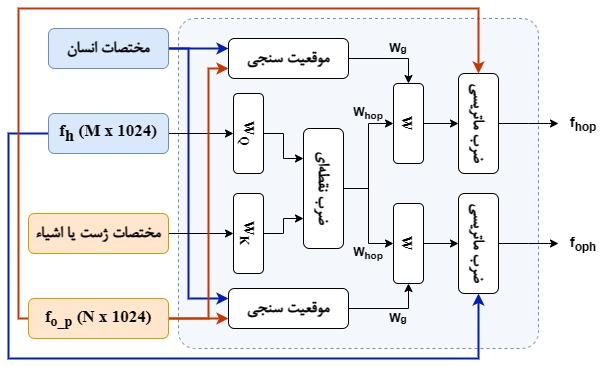
\includegraphics[width=0.7\textwidth]{majule}}
 	\caption{
 	\hl{جزییات ساختار ماژول ارتباط‌سنج}
 	}
 	\label{fig:majule}
 \end{figure}
 
 به عنوان ورودی در این ماژول ویژگی‌های انسان، ژست و اشیاء درکنار 
 \glspl{BoundingBox}
 آنها داده می‌شود و درخروجی ویژگی ترکیب شده انسان با ژست و انسان با اشیاء دریافت می‌شود. این ماژول ارتباط دوتایی را پیدا می‌کند،‌ از این رو وزن هایی که به هرکدام از روابط (مانند انسان با ژست و انسان با اشیاء) اختصاص داده می‌شود، متفاوت خواهد بود. در ادامه محاسبات انجام شده در داخل این ماژول شرح داده شده است:
 
 طبق فرمول %
 \ref{eq:ebarat_softmax}
  ورودی‌ها متشکل از بردار ویژگی انسان %
  $f_h$
   و بردار ویژگی اشیاء و یا بردار ویژگی ژست %
    $f_{o-p}$ 
    می‌باشد که درهم ضرب نقطه‌ای می‌شوند و خروجی وزن‌دار تولید می‌کنند.
 \begin{equation}
 	\label{eq:ebarat_softmax}
 	w_{hop}=\operatorname{softmax}\left(\frac{W_Q f_h \cdot W_K f_{o-p}}{\sqrt{d_k}}\right)
 \end{equation}
 در اینجا %
 $d_k$
 به عنوان یک %
\gls{ScalingFactor}
درنظر گرفته شده که گرادیان‌های پایدارتری در فاز آموزش داشته باشیم. \\
ارتباط بین انسان با ژست و انسان با اشیاء، تنها به ویژگی‌های آنها مربوط نمی‌شود بلکه به موقعیت مکانی آنها نیز بستگی دارد. بنابراین از موقعیت هندسی مرتبط با آنها نیز استفاده شده است که %
\gls{PositionEmbedding}
 صورت گیرد.
\begin{equation}
	\label{eq:scaling_factor}
	w_g=f c\left(\varepsilon_g\left(b_h, b_{o-p}\right)\right)
\end{equation}
 در اینجا %
 $f c$
 یک لایه %
\gls{FullyConnected}
،‌ %
 $b_h$
 \gls{BoundingBox}
  انسان و %
 $b_{o-p}$
 \gls{BoundingBox}
 اعضاء بدن و اشیاء را نشان می‌دهد که در یک عملیات موقعیت‌سنجی   %
 $\varepsilon_g$
 موقعیت هندسی آن‌ها محاسبه می‌شود. برای اینکه وزن‌هایی که از طریق موقعیت هندسی بدست آمده نسبت به اندازه و %
\gls{Translation}
  مقاوم باشد، ناحیه‌ای که درآن ارتباط دارند از طریق فرمول %
  \ref{eq:postion_embed}
   بدست آمده است:
\begin{equation}
	\label{eq:postion_embed}
	\left(\log \left(\frac{\left|x_h-x_{o-p}\right|}{w_h}\right)\right), \log \left(\frac{\left|y_h-y_{o-p}\right|}{h_h}\right), \log \left(\frac{w_{o-p}}{w_h}\right), \log \left(\frac{h_{o-p}}{h_h}\right)
\end{equation}
با اعمال این تغییرات روی 
 \glspl{BoundingBox}
 اصلی، مقادیر و مختصات جدیدی بدست ‌می‌آید که درنهایت این مقادیر در روند شبکه، مورد استفاده قرار می‌گیرد 
\cite{Relation_network_object}
.
 
 خروجی %
  $w_{hop}$
  که از فرمول %
 \ref{eq:ebarat_softmax}
  و مقدار %
 $w_g$
 که در از فرمول %
 \ref{eq:scaling_factor}
 بدست آمده است و همچنین ویژگی‌هایی که از بخش مختصات اشیاء و ژست بدست آمده است در یک روند ارتباط‌سنجی باهم ترکیب می‌شوند و خروجی بهینه شده بدست می‌آید:
 \begin{equation}
 	f_{h o p}=f c\left(\sum_{i=1}^n\left(\left(w_g w_{h op}\right) \cdot f_{o p}\right)\right)
 \end{equation}
شکل %
   \ref{fig:joziyat_bishtar}
   یک ساختار کلی‌تری از نحوه تشکیل شبکه در داخل بخش ارتباط‌سنج را نشان می‌دهد. 
     \begin{figure}[ht]
   	\centerline{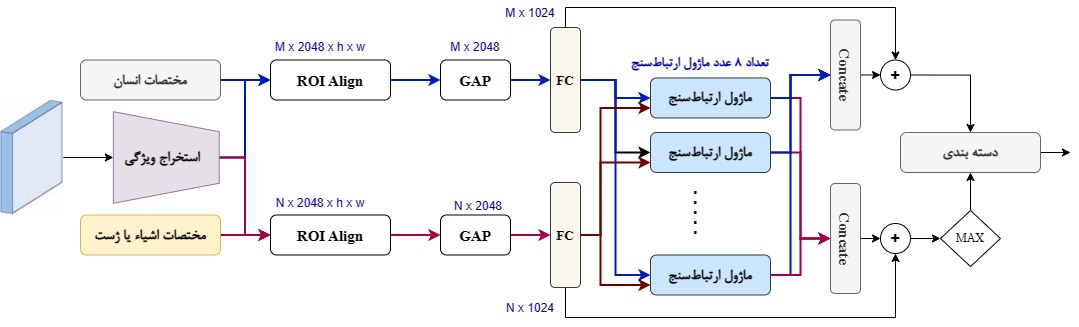
\includegraphics[width=0.95\textwidth]{joziyat_bishtar}}
   	\caption{
   		\hl{نگاه کلی‌تر به ساختار بخش ارتباط‌سنج}
   	}
   	\label{fig:joziyat_bishtar}
   \end{figure}
ابتدا تصویر وارد شبکه ResNet می‌شود که استخراج ویژگی‌ کلی از تصویر انجام گیرد. سپس از یک بخش %
\lr{RoI Align}
 می‌گذرد که ویژگی‌های ناحیه خاص از تصویر استخراج شود. در مسیر اول ویژگی‌های تصویر با کمک مختصات موقعیت بدنی انسان، خروجی مختص به بخشی از تصویر که انسان درآن حضور دارد را ‌می‌دهد. همینطور در مسیر پایین، خروجی‌ها بادرنظرگرفتن ناحیه اشیاء یا ژست تولید خواهد شد. سپس از یک GAP%
 \LTRfootnote{Global Average Pooling}
 رد می‌شود که ویژگی‌ها یک مقدار فشرده‌تر شود. درنهایت از یک لایه FC%
 \LTRfootnote{Fully Connected}
 می‌گذرد تا بار دیگر ترکیب انجام شود. سپس از چندین ماژول ارتباط‌سنج گذر می‌کند. تعداد ماژول ها 8 عدد درنظر گرفته می‌شود که از معماری %
   \gls{MultHeadAttention}
 استفاده می‌کند (
   $N_r=8$
  ). استفاده از معماری %
     \gls{MultHeadAttention}
  به شبکه این قابلیت را می‌دهد که از فضاها و دید‌های مختلف به داده نگاه کند. همچنین قابلیت موازی سازی را به شبکه اضافه می‌کند.مقدار %
   $d_k*N_r$
   برابر با اندازه بردار ویژگی‌های ورودی (1024) می‌باشد. در نهایت همه‌ خروجی‌های معماری چند شاخه به هم %
\gls{Concatenate}
    می‌شوند. البته در بخش پایین که از ژست یا اشیاء استفاده می‌شود از Max استفاده شده که یک شیء یا یک
عضو بدن در ژست که بیشترین ارتباط را با فعالیت دارد انتخاب شود.
      \subsection{تابع خطا و ترکیب امتیازات}
   بعد از اینکه ورودی از ماژول انسان - ژست و انسان - اشیاء عبور می‌کند که ویژگی‌های مرتبط با یکدیگر استخراج شود و درنهایت خروجی‌های معماری چند شاخه به هم متصل می‌شوند که یک بردار ویژگی واحد را تشکیل دهند. این بردار ویژگی از یک بخش فولی کانکتد می‌گذرد تا وارد بخش امتیازدهی شوند. 
   البته بخش دوم و سوم که مربوط به ویژگی‌های ژست و اشیاء می‌باشد، از یک %
   $max$
   عبور می‌کنند که بیشتر امتیاز بدست آمده درنظر گرفته شود. فرمول نهایی به شکل زیر خواهد بود:
   \begin{equation}
   	\operatorname{Score}(a ; h)=S_h^a+\max \left\{S_{o(1)}^a, \ldots, S_{o(n)}^a\right\}+\max \left\{S_{o(1)}^a, \ldots, S_{o(m)}^a\right\}
   \end{equation}
   
   در نهایت از یک %
   $softmax$
   عبور می‌گذرد که امتیازات ترکیب شده با جمع احتمالات برابر با یک فعالیت مورد نظر را تشخیص دهد. در روند آموزش فقط برچسب نام فعالیت مورد نظر در یک فرآیند خودناظر نیاز است که فعالیت درحال انجام را تشخیص دهد. برای تابع خطا هم از %
   $Cross$ $Entropy$ $Loss$
    استفاده شده است که در ادامه فرمول %
   \ref{eq:loss_function}
   این رابطه را نشان می‌دهد.
   \begin{equation}
   	\label{eq:loss_function}
   	L=-\log \left(\frac{\exp \left(\operatorname{Score}\left(a^{g t} ; h\right)\right)}{\sum_a \exp (\operatorname{Score}(a ; h))}\right)
   \end{equation}
   در اینجا %
    $\operatorname{Score}(a ; h)$
   امتیازات جمع‌آوری شده از فعالیت %
   $a$
   و %
   $g^t$
    در عبارت %
   $\operatorname{Score}\left(a^{g t} ; h\right)$
  نشان دهنده برچسب یا کلاسی است که فعالیت به آن تعلق دارد.		% فصل سوم: روش تحقیق
% !TeX root=../main.tex
\chapter{نتایج}
%\thispagestyle{empty} 
\label{chap:results}
\section{مقدمه} \label{introduction}
در این بخش به ارزیابی نتایج بدست آمده از الگوریتم پیشنهادی پرداخته می‌شود. بخش %
\ref{datasets}
مجموعه داده‌ های استفاده شده را شامل می‌شود. بخش %
\ref{meyar_shive_piyade}
معیار‌ها و شیوه‌های ارزیابی مرتبط با تحقیق، توضیح داده شده است. در بخش %
\ref{zojiyate_piyade}
جزییات پیاده سازی، سیستم استفاده شده و یک سری تنظیمات مربوط به مدل توضیح داده شده است.
 در بخش‌های %
\ref{natayej_majmoe_dade}
و
\ref{natayej_majmoe_dade2}
نتایج آزمایش روی مجموعه داده‌های مختلف و دو الگوریتم پیشنهادی گزارش شده است. و درنهایت بخش %
\ref{amig_negah}
یک نگاه کوتاه به خروجی مدل و نحوه نگاه مدل به مسئله بررسی شده است.

\section{‌معرفی مجموعه داده‌ها} \label{datasets}
داده های این پایان نامه، تصاویر مربوط به فعالیت های مختلف از دو مجموعه داده %
\lr{Stanford40}
 و %
 \lr{Pascal VOC‌ 2012}
 می‌باشد که اغلب کارها این دو مجموعه داده در فرآیند آموزش و ارزیابی مورد استفاده قرار می‌گیرد.
 
\lr{\textbf{ Stanford40}}
: این مجموعه داده یکی از شناخته شده ترین مجموعه داده های موجود در زمینه تشخیص فعالیت انسان در تک تصویر می‌باشد که شامل 40 کلاس از دسته بندی‌های مختلف مانند حرکات ورزشی، بازی‌ها و یک سری فعالیت های روزانه است. این مجموعه داده 4000 تصویر برای آموزش و 5530 تصویر برای ارزیابی دارد.
 
 \lr{\textbf{ Pascal VOC‌ 2012 }}
 : این مجموعه داده شامل 4588 تصویر برای 10 تا دسته بندی دارد که از این تعداد 2296 تصویر را در بخش آموزش و 2292 تصویر در بخش ارزیابی قرار دارد. درحالی که تعداد کلاس‌های این مجموعه داده کمتر از قبلی است اما چالش بیشتری نسبت به مجموعه داده قبلی دارد و تصاویر از کیفیت پایین‌تری برخوردار است. همچنین دریک تصویر ممکن است که چند شخص با فعالیت های مختلف قرار داشته باشد که این یک چالش اساسی است.
 
 دربین این دوتا مجموعه داده، %
 \lr{Stanford40}
 بیشتر از %
 \lr{Pascal VOC}
 مورد استفاده قرار می‌گیرد. هردوی این مجموعه داده‌ها نواحی انسان را مشخص کرده اند و ناحیه‌ی اشیاء از کدهای منتشر شده کار%
 \cite{Human_object_relation_action}
 قابل استفاده است.
 
 \section{‌معیار و شیوه‌های ارزیابی} \label{meyar_shive_piyade}
 در مسائل مختلف معیارهاي ارزیابی متفاوتی استفاده می‌شود، اما برخی معیارهاي ارزیابی به دلیل استاندارد بودن در بسیاري پژوهش‌ها مورد استفاده قرار می‌گیرند. در این پایان نامه نیز سعی شده است تا الگوریتم پیشنهادي با برخی از این معیارهای کمی مورد ارزیابی قرار گیرد.
 
 برای استفاده از معیار‌های کمی ارزیابی،‌ دوحالت را برای فعالیت انسان در نظر می‌گیریم،‌ یا فعالیت بدست آمده مربوط با تصویر است یا نامرتبط با آن است. اگر مرتبط باشد و بیانگر همان فعالیت درحال انجام باشد، مثبت و اگر فعالیتی وجود نداشته باشد، منفی درنظر گرفته می‌شود.
 
\textbf{مثبت درست}
 \LTRfootnote{True Positive}
 : زمانی رخ می‌دهد که مدل فعالیتی را درتصویر تشخیص می‌دهد که در برچسب نیز همان فعالیت است و نشان می‌دهد که فعالیت در تصویر و برچسب یکسان است.
 
\textbf{مثبت غلط}
\LTRfootnote{False Positive}
: زمانی رخ می‌دهد که مدل فعالیتی را در تصویر تشخیص می‌دهد اما در مجموعه داده‌های ما فعالیتی برای آن تعریف نشده یا وجود ندارد.

\textbf{منفی درست}
\LTRfootnote{True Negative}
: زمانی رخ می‌دهد که مدل عدم وجود فعالیت را تشخیص می‌دهد و برچسب یا مجموعه داده اصلی مانیز عدم حضور فعالیت را نشان می‌دهد.

  \textbf{منفی غلط}
  \LTRfootnote{False Negative}
  : زمانی رخ می‌دهد که مدل عدم وجود فعالیت را تشخیص می‌دهد اما برچسب وجود فعالیت را نشان می‌دهد.
  
  \textbf{\gls{Accuracy}}
  : یکی از معیارهای ارزیابی متداول برای اندازه‌گیری عملکرد یک مدل طبقه‌بندی است. این معیار نسبت تعداد نمونه‌هایی که به درستی طبقه‌بندی شده‌اند (هم پیش‌بینی‌های مثبت و هم پیش‌بینی‌های منفی) به تعداد کل نمونه‌ها را نشان می‌دهد.
\begin{equation}
	\text { Accuracy }=\frac{T P+T N}{T P+T N+F P+F N}
\end{equation}
\textbf{\gls{Precision}}
 : تعداد نمونه‌هایی که از یک کلاس خاص به درستی تشخیص داده شده‌اند، نسبت به تعداد کل نمونه‌هایی که به اشتباه به آن کلاس اختصاص داده شده‌اند.
  \begin{equation}
  	\text { Precision }=\frac{T P}{T P+F P}
  \end{equation}
  \textbf{\gls{Recall}}
 : یکی از معیارهای ارزیابی عملکرد مدل‌های دسته‌بندی است که نسبت تعداد نمونه‌های مثبتی را که به درستی تشخیص داده شده‌اند به تعداد کل نمونه‌های مثبت در داده‌های آزمون را نشان می‌دهد.
  \begin{equation}
  	\text { Recall }=\frac{T P}{T P+F N}
  \end{equation}
    \textbf{میانگین متوسط دقت}
  \LTRfootnote{Mean Average Precision}
: در مسائل تشخیص فعالیت انسان در تک تصویر، معیار mAP به منظور ارزیابی عملکرد مدل‌های دسته‌بندی استفاده می‌شود. این معیار از AP%
 \LTRfootnote{Average Precision}
 ها برای هر کلاس محاسبه می‌شود و سپس میانگین آن‌ها برای تمام کلاس‌ها گرفته می‌شود. mAP نشان می‌دهد که مدل در تشخیص فعالیت مختلف در تصاویر چقدر موفق بوده است.
 \begin{equation}
 	\mathrm{mAP}=\frac{1}{N} \sum_{i=1}^N \mathrm{AP}_i
 \end{equation}
     \textbf{\gls{ConfusionMatrix}}
: ماتریس درهم ریختگی یک ابزار ارزیابی است که برای اندازه‌گیری عملکرد مدل‌های دسته‌بندی استفاده می‌شود. این ماتریس برای مدل‌هایی که به صورت دودویی (با دو کلاس مثبت و منفی) طبقه‌بندی می‌کنند، به کار می‌رود. اما می‌توان آن را برای مسائل با چند کلاس نیز گسترش داد. شکل %
\ref{fig:confution_matrix_explain}
نحوه چینش ماتریس درهم ریختگی را نشان می‌دهد. البته طول ماتریس ممکن است متفاوت باشد اما همچنان این نوع ساختار درآن حفظ می‌شود.
\begin{figure}[ht]
	\centerline{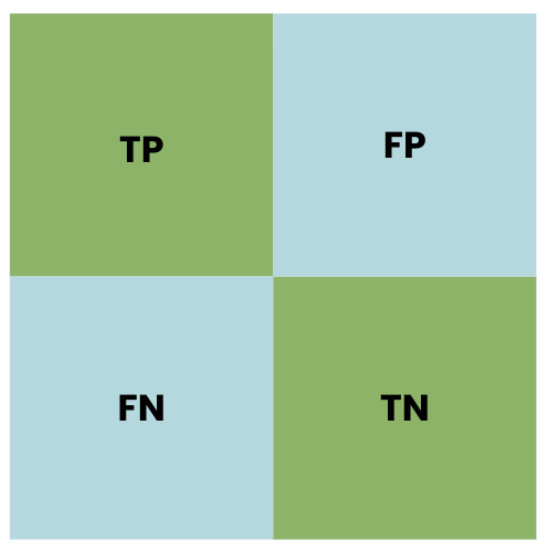
\includegraphics[width=0.2\textwidth]{confution_matrix_explain}}
	\caption{نمونه ماتریس درهم ریختگی}
	\label{fig:confution_matrix_explain}
\end{figure}
\vspace{-10pt}
 \section{‌جزئیات پیاده سازی}\label{zojiyate_piyade}
تمامی آزمایشات این پایان نامه با زبان پایتون کدنویسی شده و در سیستم عامل لینوکس اوبونتو و روی کامپیوتر با مشخصات حافظه داخلی 16 گیگابایت و گرافیک 4 گیگابایت تست شده است. آموزش های مدل روی سیستم مجازی %
\lr{Google Colab}
انجام شده است که این سیستم گرافیک تا 14 گیگابایت را در اختیارمان قرار داد. الگوریتم معرفی شده در چارچوب MXNet پیاده سازی شده است.\\
درمرحله آموزش %
\lr{Loss Function} 
که استفاده شده %
\lr{Cross-Entropy}
است و بهینه ساز مورد نظر نیز‌ %
\gls{StochasticGradientDescent}
انتخاب شده است. نرخ یادگیری را %
\rl{4e-4}
 ،  %
 \gls{Momentum}
 9.0
 و تعداد حلقه های آموزش 15 درنظر گرفته شده است. همچنین نرخ آموزش در این 15 تکرار از $3*10^{-5}$ به $1*10^{-6}$ کاهش می‌یابد.\\
در بخش بدنه اصلی مدل از %
\lr{ResNet50}
استفاده شده است که فرآیند استخراج ویژگی را انجام می‌دهد. نقاط کلیدی بدن انسان نیز با دو الگوریتم yolo و mmpose استخراج شده است.
 \section{نتایج روی مجموعه داده ‌های  \lr{Stanford40}} \label{natayej_majmoe_dade}
 ارزیابی نتایج دو الگوریتم پیشنهادی در جدول %
 \ref{tab:jadval_degat_all}
 نشان داده شده است.
 \begin{table}[h!]
 	\centering
	\begin{tabularx}{0.8\textwidth} { 
			  >{\raggedleft\arraybackslash}X 
			 >{\raggedleft\arraybackslash}X 
			 p{2cm} >{\raggedleft\arraybackslash}X  }
		\hline
 \textbf{الگوریتم} & \textbf{بدنه اصلی} & \textbf{میانگین دقت (mAP)}\\
		\hline
		Attention %
		\cite{Multi_branch_Attention_Recg_still}
		& \lr{VGG 16} & \lr{90.7} \\
		R*CNN %
		\cite{contextual_action_rcnn}
		& \lr{VGG 16} & \lr{90.9} \\
		Part Action %
		\cite{Single_image_semantic_body}
		& \lr{ResNet-50} & \lr{91.2} \\
		Loss Guided %
		\cite{Loss_guided_actv_attention}
		& \lr{ResNet-50} & \lr{91.1} \\
		KPs-Assisted %
		\cite{a_key_points_assisted_net}
		& \lr{EfficientNetV2} & \lr{91.8} \\
		Relation %
		\cite{Human_object_relation_action}
		& \lr{ResNet-50} & \lr{\textbf{93.1}} \\
		\hline
		روش پیشنهادی + ارتباط‌سنج
		& \lr{ResNet-50} & \lr{\textbf{92.6}} \\
		روش پیشنهادی + LAD
		& \lr{ResNet-50} & \lr{\textbf{92.7}} \\
		\hline
	\end{tabularx}
	\caption{دقت روش‌های مختلف روی مجموعه داده \lr{Stanford40}}
	\label{tab:jadval_degat_all}
\end{table}
همانطورکه آزمایش شد،‌ استفاده از ژست در این مجموعه داده منجربه دقت پایین تری نسبت به روش %
\cite{Human_object_relation_action}
شد. همچنین نبود وزن‌های‌ اولیه آماده در مدل های قبلی و مدل پیشنهادی کار آموزش مدل‌ها با کندی پیش رفت که صرف هزینه زمانی زیادی شد. البته از بدنه قوی تری نیز استفاده نشد زیرا مدل‌های قبلی از این بدنه برای ارزیابی استفاده کردند و ما نیز از این بدنه استفاده کردیم که دریک شرایط برابر مقایسه انجام شود.
با این حال استفاده از ژست مخصوصا اضافه کردن بردار ویژگی بهبود یافته توصیف کننده زاویه بدن%
\LTRfootnote{iLAD}
 یک مقدار عملکرد بهتری نسبت به روش ارتباط‌سنج گزارش داد.
 
 ماتریس درهم‌ریختگی یک ابزار مفید در ارزیابی نتایج می‌باشد. شکل %
\ref{fig: confution_matrix_std_m}
ماتریس درهم‌ریختگی روش پیشنهادی با ارتباط‌سنج نشان می‌دهد.
  \begin{figure}[ht]
  	\centerline{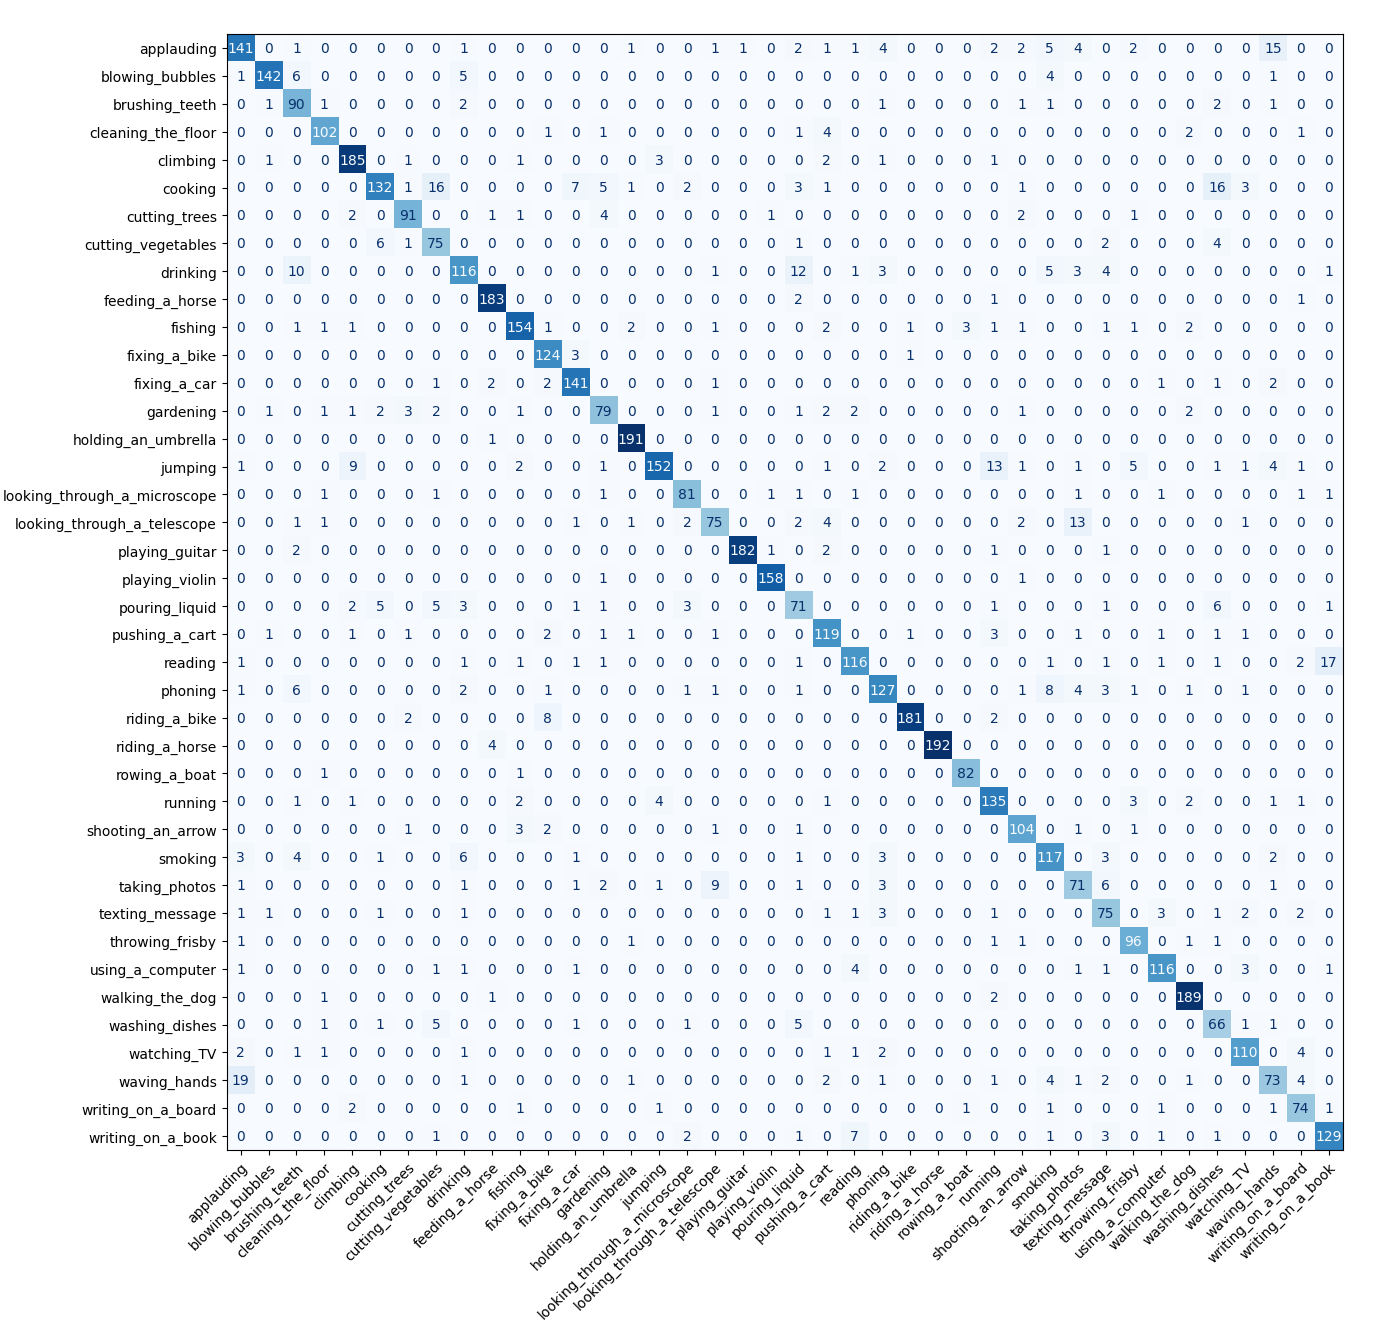
\includegraphics[width=0.9\textwidth]{confution_matrix_std40}}
  	\caption{ماتریس درهم ریختگی روش ارتباط‌سنج روی \lr{Stanford40}}
  	\label{fig: confution_matrix_std_m}
  \end{figure}
  
  طبق این نتایج بدست آمده، فعالیت "تشویق کردن" با 15 دسته‌بندی اشتباه و "تکان دادن دست" با 19 اشتباه جزء فعالیت‌های دشوار برای این مدل به شمار می‌روند. علت این دسته‌بندی نادرست نزدیک بودن دو فعالیت در حالت دست ها است. به دلیل نبودن اطلاعات زمانی و حرکتی مدل نمی‌تواند تفکیک درستی از حرکت دست ‌ها و تخمین فعالیت داشته باشد.\\
همچنین فعالیت "آشپزی کردن" با 16 دسته‌بندی نادرست از کلاس "شستن ظرف" نشان می‌دهد که وجود ظرف درهر دو فعالیت باعث گمراهی ‌مدل شده است. دراینجا نیز نبود اطلاعات حرکتی عامل اصلی این دسته‌بندی نادرست است.

  در شکل %
  \ref{fig: confution_matrix_std40_lad}
   ماتریس درهم‌ریختگی برای روش توصیف کننده زاویه بدن نشان داده شده است.
    \begin{figure}[ht]
  	\centerline{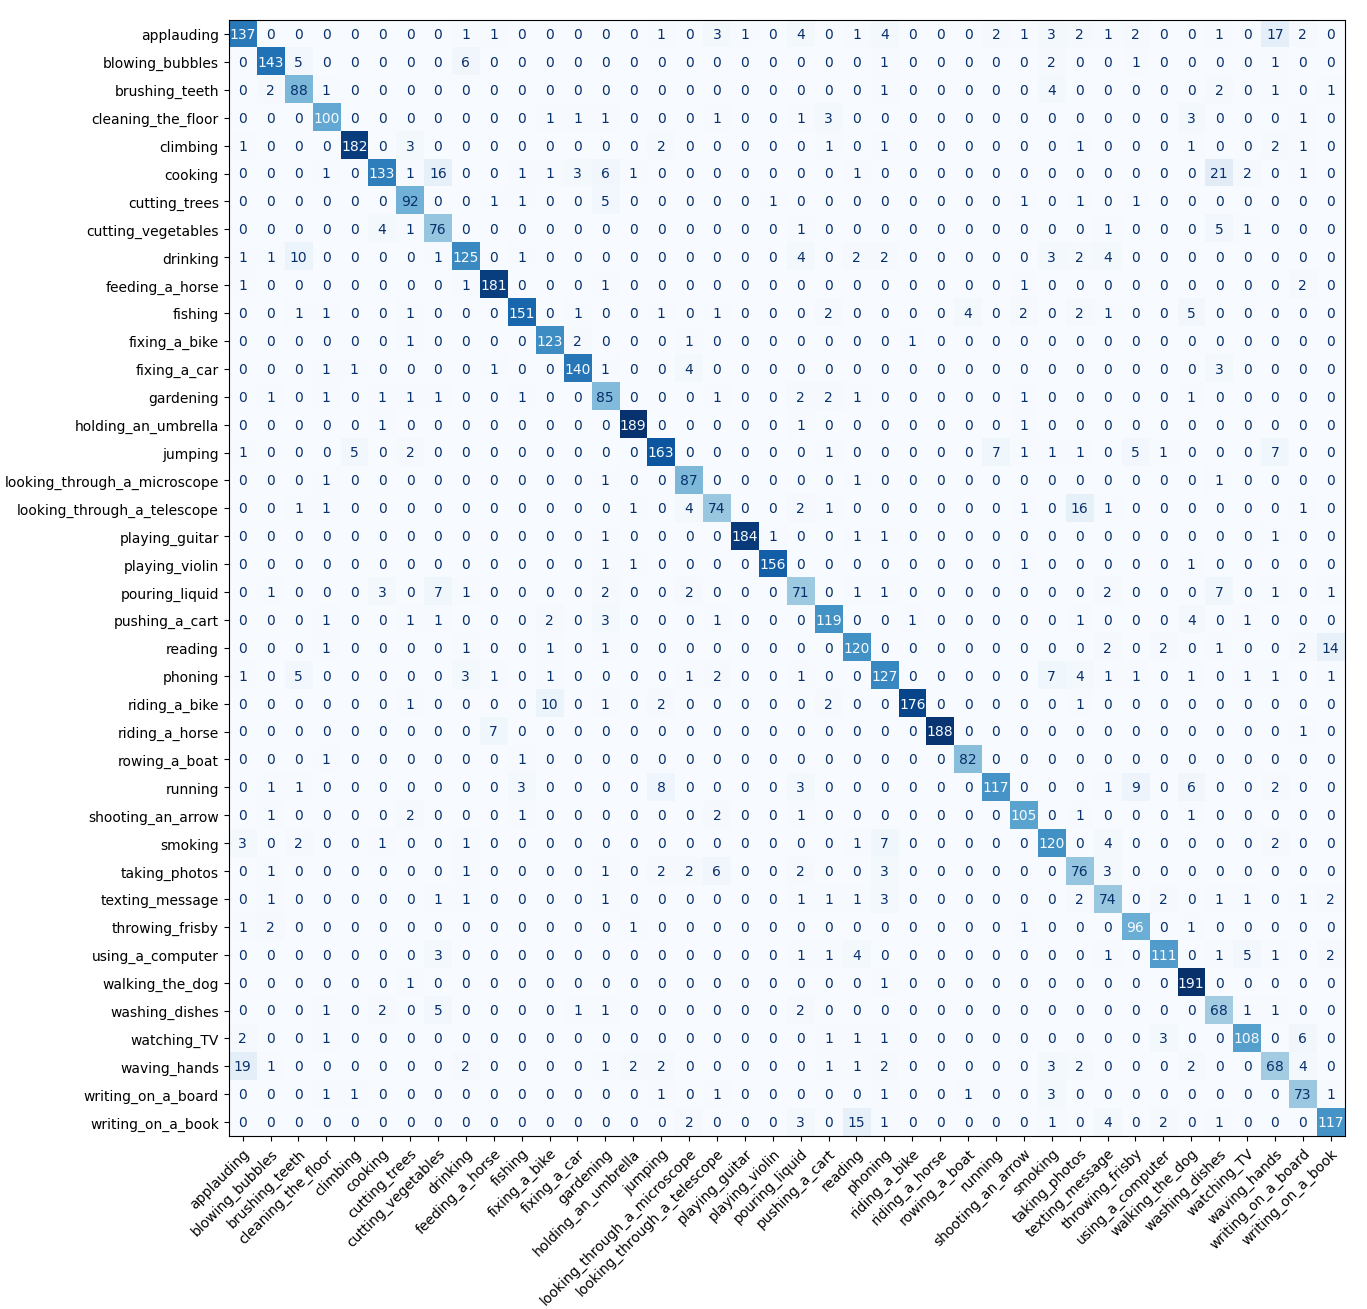
\includegraphics[width=0.9\textwidth]{confution_matrix_std40_lad}}
  	\caption{ماتریس درهم ریختگی روش توصیف کننده زاویه بدن روی \lr{Stanford40}}
  	\label{fig: confution_matrix_std40_lad}
  \end{figure}
  همانطور که در شکل مشخص است، بیشتری دسته بندی نادرست مربوط به فعالیت "آشپزی کردن" است که 21 تصویر از فعالیت "شستن ظرف" را به اشتباه فعالیت "آشپزی کردن" پیش بینی کرده است. این نشان می‌دهد که فعالیت های "آشپزی کردن" و "شستن ظرف" جزء سخت ترین فعالیت‌ ها در این مجموعه داده است.
دو فعالیت "اسب سواری" و "ویالون زدن" جز دوتا فعالیتی هستند که کمترین خطا را داشتند و هر دو مدل به درستی توانسته‌‌اند این دو را دسته بندی کنند.
 \begin{table}[h!]
	\centering
	\fontsize{10pt}{10pt}\selectfont
	\begin{tabularx}{0.8\textwidth} { 
			| >{\raggedleft\arraybackslash}X 
			| >{\raggedleft\arraybackslash}X 
			| >{\raggedleft\arraybackslash}X
			| >{\raggedleft\arraybackslash}X |
			 }
		\hline
		\textbf{بیشترین ها} & \textbf{دقت (\%)} & \textbf{کمترین ها} & \textbf{دقت (\%)} 
		\\
		\hline
		اسب سواری &
		\lr{99.9} &
		تکان دادن دست &
		\lr{73.2}\\
		\hline
		ویالون زدن &
		\lr{99.9} &
		سرریز کردن آب &
		\lr{79.5} \\
		\hline
		گیتار زدن &
		\lr{99.8} &
		عکس گرفتن &
		\lr{81.0} \\
		\hline
	\end{tabularx}
	\caption{ سه تا از بیشترین و کمترین دقت ها روی \lr{Stanford40}}
	\label{tab:jadval_degat_best_std}
\end{table}
\section{نتایج روی مجموعه داده‌ های \lr{VOC 2012}}\label{natayej_majmoe_dade2}
این مجموعه داده چالش بیشتری نسبت به مجموعه داده %
\lr{Stanford40}
 دارد. نتایج ارزیابی روی این مجموعه داده در جدول %
  \ref{tab:jadval_degat_all_voc}
  نشان داده شده است.
  \begin{table}[h!]
  	\centering
  	\fontsize{10pt}{10pt}\selectfont
  	\begin{tabularx}{0.99\textwidth} { 
  			p{2.3cm}>{\raggedleft\arraybackslash}X 
  			>{\raggedleft\arraybackslash}X 
  			>{\raggedleft\arraybackslash}X 
  			>{\raggedleft\arraybackslash}X 
  			>{\raggedleft\arraybackslash}X 
  			>{\raggedleft\arraybackslash}X 
  			>{\raggedleft\arraybackslash}X 
  			>{\raggedleft\arraybackslash}X 
  			>{\raggedleft\arraybackslash}X 
  			>{\raggedleft\arraybackslash}X 
  			| >{\raggedleft\arraybackslash}X 
  			>{\raggedleft\arraybackslash}X  }
  		\hline
  		\textbf{الگوریتم} & \textbf{پریدن} & \textbf{تلفن زدن} & \textbf{ساز زدن} & \textbf{خواندن} & \textbf{دوچرخه سواری} & \textbf{اسب سواری} & \textbf{دویدن} & \textbf{عکس گرفتن} & \textbf{استفاده کامپیوتر} & \textbf{راه رفتن} & \textbf{دقت}
  		\\
  		\hline
  		Attention %
  		\cite{Multi_branch_Attention_Recg_still}
  		& \lr{87.8} & \lr{78.4} & \lr{93.7} & \lr{81.1} & \lr{95.0} & \lr{97.1} & \lr{\textbf{96.0}} & \lr{85.5} & \lr{93.1} & \lr{73.4} & \lr{87.1}
  		\\
  		R*CNN %
  		\cite{contextual_action_rcnn}
  		& \lr{88.9} & \lr{79.9} & \lr{95.1} & \lr{82.2} & \lr{96.1} & \lr{97.8} & \lr{87.9} & \lr{85.3} & \lr{94.0} & \lr{71.5} & \lr{87.9}\\
  		Part Action %
  		\cite{Single_image_semantic_body}
  		& \lr{89.6} & \lr{86.9} & \lr{94.4} & \lr{\textbf{88.5}} & \lr{94.9} & \lr{97.9} & \lr{91.3} & \lr{87.5} & \lr{92.4} & \lr{76.4} & \lr{90.0} \\
  		Relation %
  		\cite{Human_object_relation_action}
  		& \lr{89.2} & \lr{89.8} & \lr{96.5} & \lr{87.6} & \lr{\textbf{98.2}} & \lr{99.1} & \lr{92.3} & \lr{91.6} & \lr{95.2} & \lr{79.2} & \lr{91.9} \\
  		Patch %
  		\cite{patch_boxless_action}
  		& \lr{89.0} & \lr{86.6} & \lr{95.0} & \lr{87.7} & \lr{95.7} & \lr{96.7} & \lr{92.3} & \lr{82.0} & \lr{95.6} & \lr{72.7} & \lr{89.3} \\
  		\hline
پیشنهادی(ارتباط‌سنج)
  		& \lr{90.7} & \lr{89.3} & \lr{95.6} & \lr{86.7} & \lr{97.7} & \lr{98.8} & \lr{93.2} & \lr{90.5} & \lr{\textbf{95.6}} & \lr{\textbf{80.2}} & \lr{91.9} \\
  		پیشنهادی(LAD)
  		& \lr{\textbf{91.5}} & \lr{\textbf{90.9}} & \lr{\textbf{97.0}} & \lr{87.4} & \lr{97.5} & \lr{\textbf{99.1}} & \lr{93.1} & \lr{\textbf{92.5}} & \lr{95.1} & \lr{78.9} & \lr{\textbf{92.33}} \\
  		\hline
  	\end{tabularx}
  	\caption{دقت روش‌های مختلف روی مجموعه داده \lr{VOC 2012}}
  	\label{tab:jadval_degat_all_voc}
  \end{table}
 همانطور که طبق جدول %
  \ref{tab:jadval_degat_all_voc}
  مشاهده می‌کنید، روش پیشنهادی توصیف کننده زاویه بدن روی این مجموعه داده عملکرد بسیاری خوبی از خود نشان داده است. در فعالیت های "پریدن" ، "تلفن زدن" ، "ساز زدن" ، "اسب سواری" ، "عکس گرفتن" بیشترین دقت ها را بین رقبای خود بدست آورده است و میانگین متوسط دقت 33.92\% بیشترین دقت در این بین می‌باشد.
  
  در تصویر %
\ref{fig: confiution_matrixvoc}
و 
\ref{fig: confution_matrix_voclad}
ماتریس درهم‌ریختگی برای روش ارتباط‌سنج و توصیف کننده زاویه بدن نشان داده شده است. در این دو تصویر دو فعالیت "دویدن" و "راه رفتن" چندین نمونه دسته‌بندی اشتباه داشتند. دلیل اصلی این اشتباهات نیز نبود را می‌توان نبود اطلاعات حرکتی و زمانی در تک تصویر معنا کرد. زیر مرز باریکی بین دویدن و راه رفتن در تصویر وجود دارد. دسته "موارد دیگر" به دلیل مشخص نبودن نوع فعالیت و تصاویر به هم ریخته و نامنظم نادیده گرفته می‌شود. \\
نمودار %
\ref{fig: nemodar_natije_relation_pish}
تفاوت بین روش پیشنهادی با توصیف کننده زاویه بدن و مقاله %
\cite{Human_object_relation_action}
را نشان می‌دهد.

\begin{figure}[ht]
	\centerline{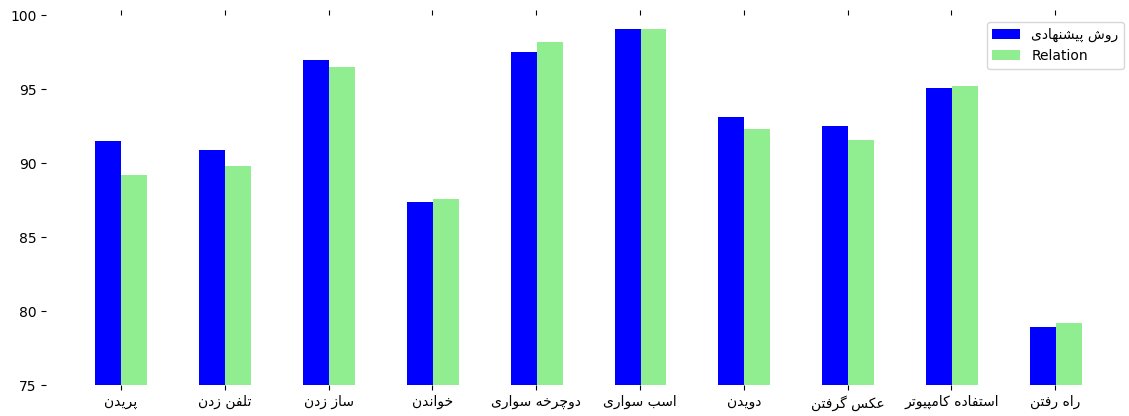
\includegraphics[width=0.9\textwidth]{nemodar_r_p}}
	\caption{نمودار مقایسه نتایج روش پیشنهادی توصیف کننده بدن با \lr{Relation}}
	\label{fig: nemodar_natije_relation_pish}
\end{figure}
\begin{figure}[ht]
	\centerline{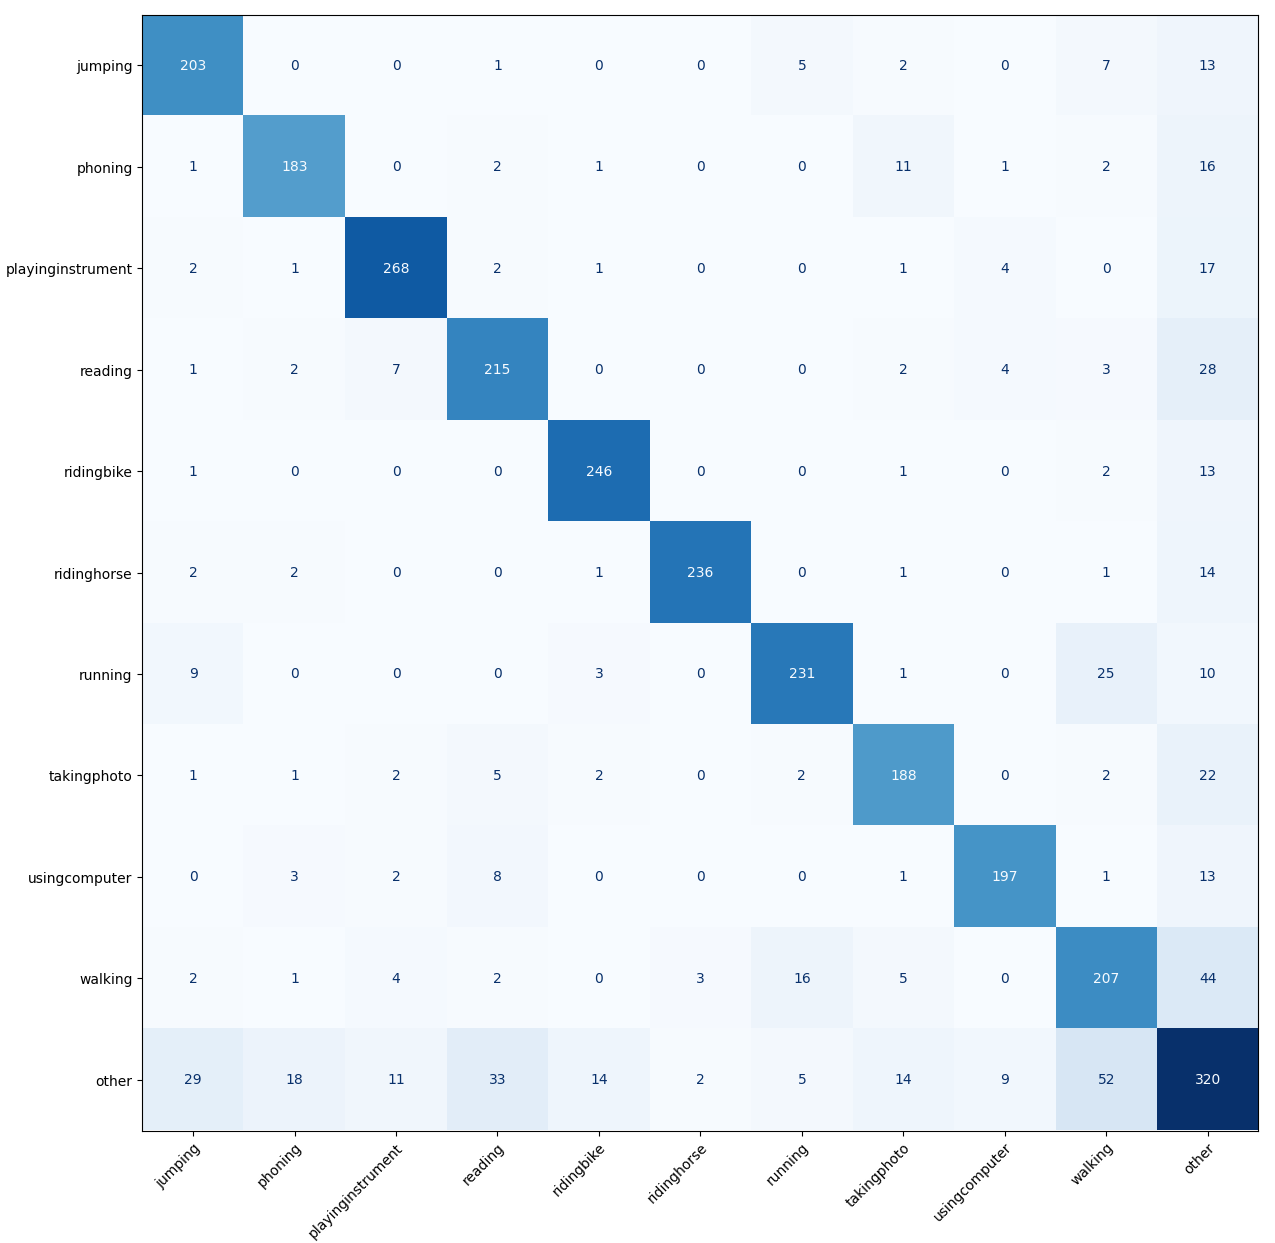
\includegraphics[width=0.66\textwidth]{confiution_matrix_voc}}
	\caption{ماتریس درهم ریختگی روش ارتباط‌سنج روی \lr{Voc 2012}}
	\label{fig: confiution_matrixvoc}
\end{figure}
\begin{figure}[ht]
	\centerline{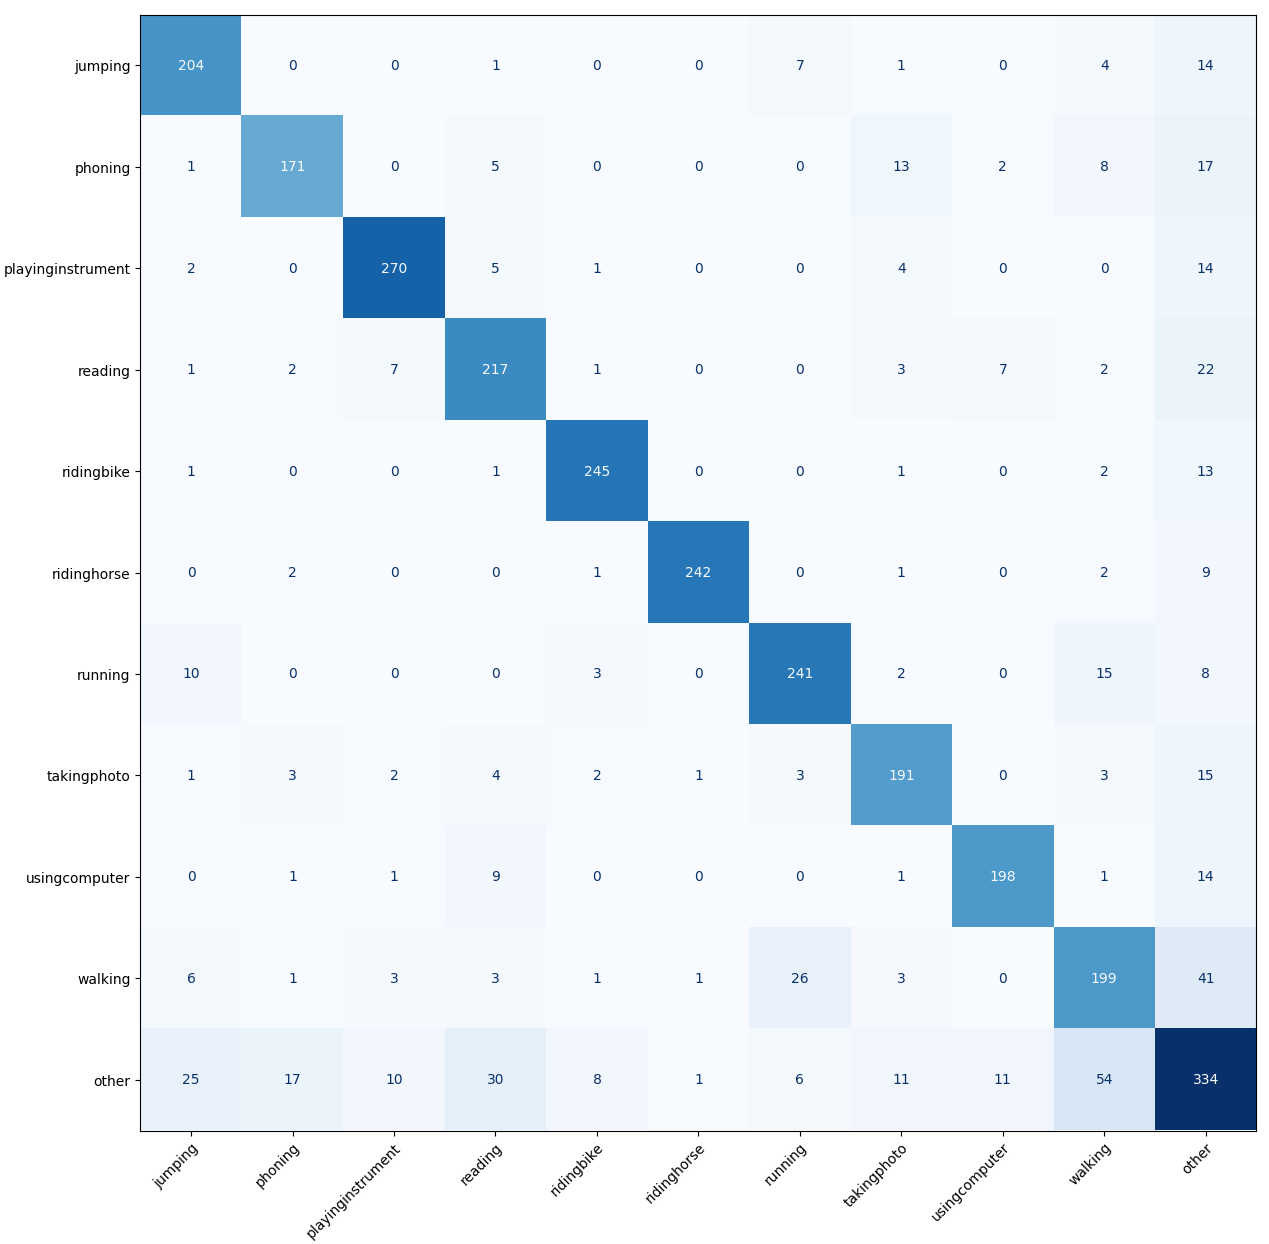
\includegraphics[width=0.66\textwidth]{confution_matrix_voc_lad}}
	\caption{ماتریس درهم ریختگی روش توصیف کننده زاویه بدن روی \lr{Voc 2012}}
	\label{fig: confution_matrix_voclad}
\end{figure}
\section{نگاه عمیق تر و تصویرسازی}\label{amig_negah}
تصاویر %
\ref{fig: confiution_matrixvoc}
از خروجی مدل در بخش %
\gls{Classifier}
قرار گرفته است. این تصاویر نشان می‌دهد که مدل به کدام بخش از ناحیه‌ی تصویر در جهت تشخیص فعالیت،‌ بیشترین توجه را دارد و بیشترین امتیاز را به کدام ناحیه اختصاص می‌دهد.
تصویر %
\ref{fig: myplot_voc}
یک نمونه تصویر از این مجموعه داده است که نشان می‌دهد 3 فعالیت در یک تصویر درحال انجام است که مدل تشخیص نقاط کلیدی بدن توانسته به صورت مجزا برای هرکدام ناحیه‌های بدن را ترسیم کند.
\begin{figure}[ht]
	\centerline{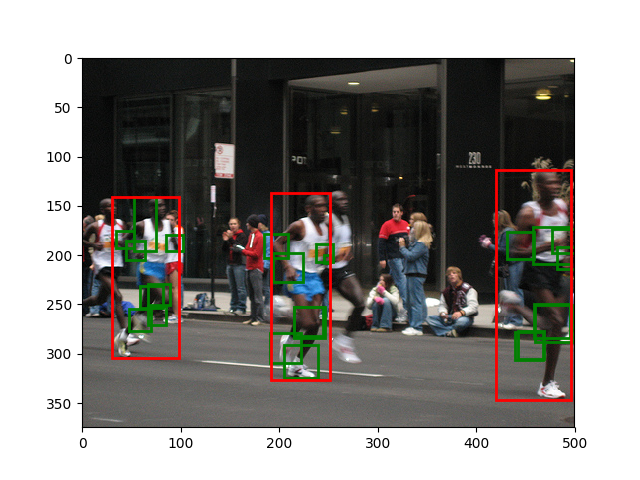
\includegraphics[width=0.8\textwidth]{myplot_voc}}
	\caption{نمونه تصویر فعالیت در \lr{Voc 2012}}
	\label{fig: myplot_voc}
\end{figure}

تصاویر %
\ref{fig:res_for_medioum images}
 از پیش‌بینی مدل در بخش ارتباط‌سنج نشان داده شده است. ناحیه سبز رنگ، ناحیه برجسته اشیاء و ناحیه آبی رنگ ناحیه برجسته اجزاء بدن را نشان می‌دهد.
   \begin{figure}
 	\centering
 	\subfloat[ ]{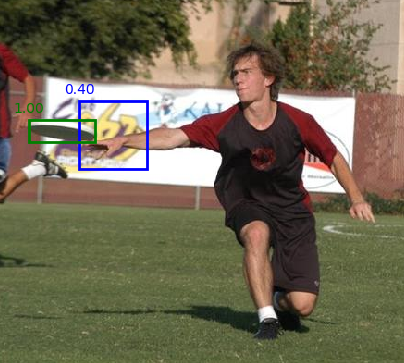
\includegraphics[width=0.24\textwidth]{res_playing}}
 	\hfill
 	\subfloat[ ]{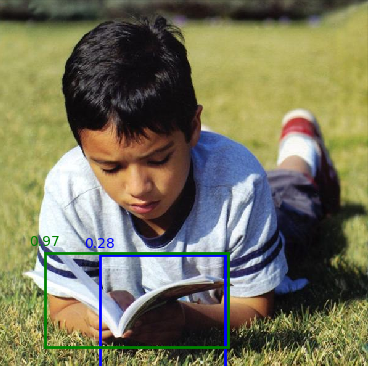
\includegraphics[width=0.24\textwidth]{res_reading}}
 	\hfill
 	\subfloat[ ]{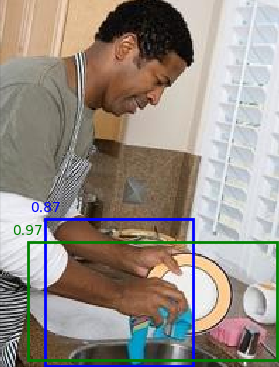
\includegraphics[width=0.24\textwidth]{res_washing_dishes}}
 	\hfill
 	\subfloat[ ]{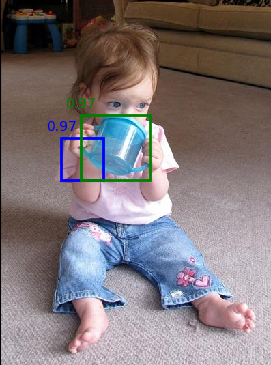
\includegraphics[width=0.24\textwidth]{res_drinking}}
 	\\
 	\subfloat[ ]{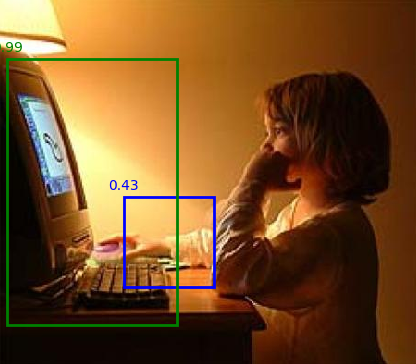
\includegraphics[width=0.24\textwidth]{res_computer}}
 	\hfill
 	\subfloat[ ]{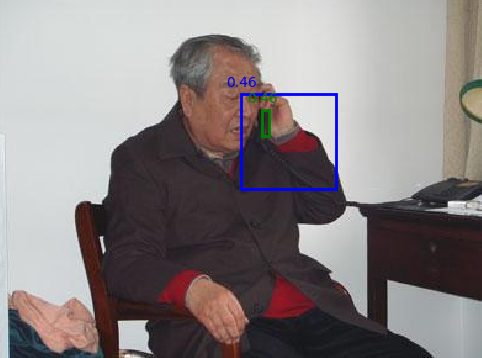
\includegraphics[width=0.24\textwidth]{res_phone_calling}}
 	\hfill
 	\subfloat[ ]{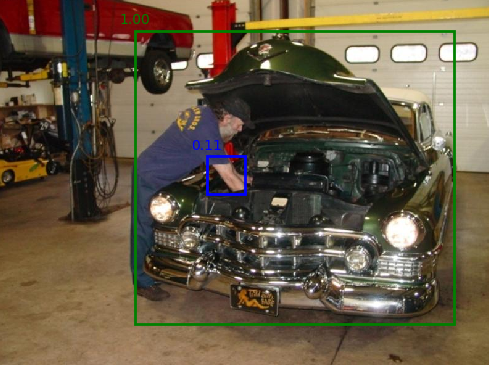
\includegraphics[width=0.24\textwidth]{res_fixing_car}}
 	\hfill
 	\subfloat[ ]{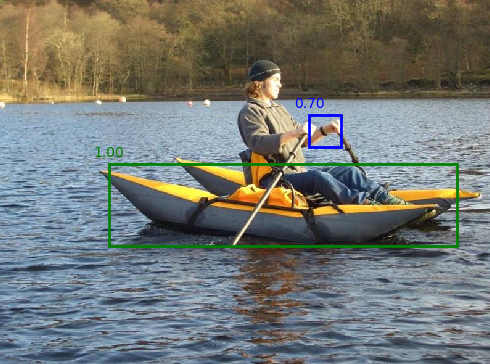
\includegraphics[width=0.24\textwidth]{res_gayeg_savari}}
 	\hfill
 	\caption{تصاویر %
 		\gls{BoundingBox}
 		 ژست بدست آمده از نقاط کلیدی}
 	\label{fig:res_for_medioum images}
 \end{figure}
همانطور که در این تصاویر مشاهده می‌شود، "دست" بیشتر عامل تاثیرگذار در تشخیص فعالیت‌هایی است که نیاز به استفاده از "دست" بیشتر است. همچنین شیء که بیشترین ارتباط را با فعالیت مورد نظر دارد نیز مشخص کرده است.

در تصاویر %
\ref{fig: confiution_matrixvoc}
یک سری از پیش‌ بینی‌های نادرست نشان داده شده است. تصاویر "آ" و "د" تقریبا باهم مشابه هستند و درهر دو دست بالا قرار گرفته است. ممکن است عاملی باشد که شبکه خروجی جا به جا تولید کرده باشد. همچنین جفت تصاویر "ب" و"ه" ظرف و شکل دست در هنگام ظرف شستن و آشپزی کردن باعث گمراهی شبکه شده و"ج" و "و" نیز به همین ترتیب. تصویر "ج" به دلیل اینکه شخص خودکار در دست گرفته است باعث شده شبکه خروجی نوشتن کتاب را پیش بینی کند.
  \begin{figure}
	\centering
	\subfloat[\color{red}تکان دادن دست
	]{
\includegraphics[width=0.25\textwidth]{applauding_216}}
	\hfill
	\subfloat[\color{red}آشپزی کردن
	]{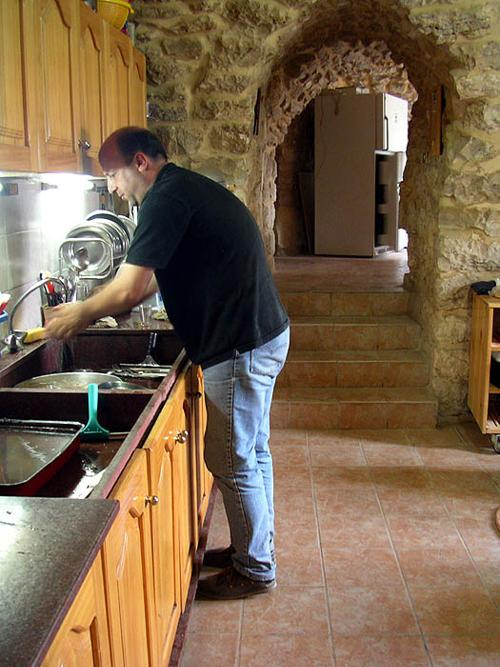
\includegraphics[width=0.25\textwidth]{washing_dishes_093}}
	\hfill
	\subfloat[\color{red}نوشتن کتاب]{
\includegraphics[width=0.30\textwidth]{reading_011}}
	\\
	\subfloat[\color{red}تشویق کردن]{
\includegraphics[width=0.25\textwidth]{waving_hands_210}}
	\hfill
	\subfloat[\color{red}ظرف شستن
	]{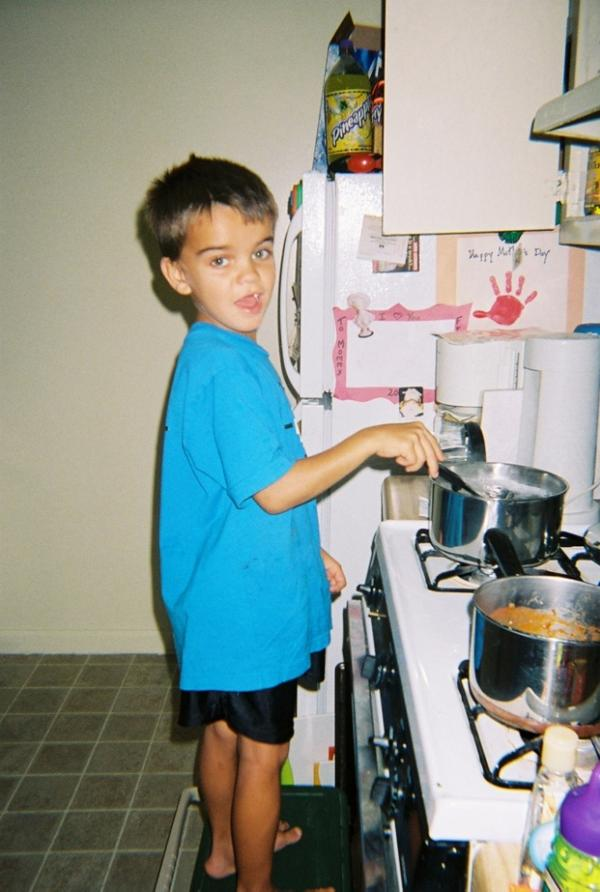
\includegraphics[width=0.25\textwidth]{cooking_006}}
	\hfill
	\subfloat[\color{red}خواندن کتاب
	]{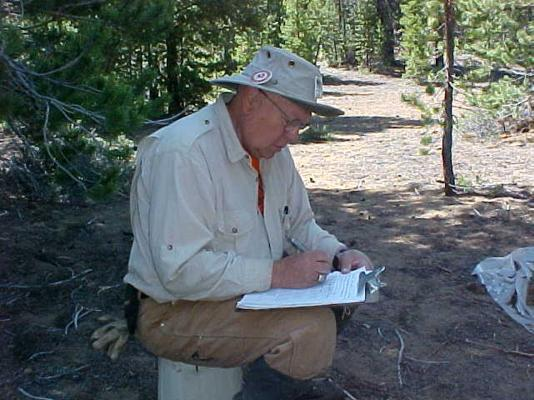
\includegraphics[width=0.30\textwidth]{writing_on_a_book_141}}
	\hfill
	\caption{تصاویری از پیش بینی‌های نادرست شبکه}
	\label{fig:res_for_false_prediction}
\end{figure}
 		% فصل چهارم: نتایج
% !TeX root=../main.tex
\chapter{نتیجه‌گیری و کارهای آتی}
%\thispagestyle{empty} 
\section{مقدمه}
تشخیص فعالیت انسان در تک تصویر به عنوان یکی از حوزه‌های پررنگ و مهم در زمینه هوش مصنوعی و بینایی ماشین مطرح است. این حوزه تحقیقاتی به تحلیل و تفسیر عملکرد انسان در محیط‌های مختلف و در زمان واقعی می‌پردازد. از آنجایی که فعالیت‌های انسانی حاصل ترکیبی پیچیده از حرکات بدنی و ارتباطات انسانی است، تشخیص این فعالیت‌ها در تک تصویر یک چالش فنی و معمولاً پیچیده است.

با توجه به پیچیدگی رفتار‌های انسانی،‌ تشخیص فعالیت انسان در تک تصویر می‌تواند در تشخیص الگو‌های رفتاری،‌ عادات و وضعیت‌های روانی افراد کمک کننده باشد. همچنین با پیشرفت تکنولوژی و توسعه روش‌های هوش مصنوعی و بینایی ماشین، امکانات بهتری برای تشخیص و تحلیل فعالیت‌های انسان در تک تصویر ایجاد شده است که این موضوع می‌تواند به توسعه کاربرد‌های جدید  و بهبود کارایی ماشین‌ها در تعامل با محیط کمک کنند. با توجه به این دلایل، تحقیقات در زمینه تشخیص فعالیت انسان در تک تصویر ارزشمند و حیاتی به نظر می‌رسد که می‌تواند به توسعه‌ی دانش و فناوری‌های مرتبط و بهبود شرایط زندگی انسان کمک کنند.

دراین پایان نامه از مکانیزم توجه که بخش مهمی از شبکه ترنسفرمر را شامل می‌شود، در کاربرد ارتباط‌سنج استفاده شد. از این شبکه در تعامل با مسیر توصیف کننده برای ژست استفاده شد که در این مسیر توصیف کننده ژست، مختصات ژست و ویژگی‌های استخراج شده از تصویر با هم ترکیب شدند و یک بردار ویژگی بهینه جهت تشخیص فعالیت ایجاد کردند. با درنظر گرفتن این مسیر نتیجه روی مجموعه داده %
\lr{VOC 2012}
دقت %
\lr{92.33\%}
را نشان داد که در حالتی که این مسیر درنظر گرفته نمی‌شود نزدیک %
\lr{4.4}
درصد بهتر عمل کرد که نشان می‌دهد استفاده از ژست انسان موجب بهتر شدن دقت تشخیص فعالیت می‌شود.

طبق نتایج بدست آمده مدل بیشتر از نقاط کلیدی ناحیه‌ی "دست" استفاده کرده است. البته بستگی به فعالیت دارد اما با این حال نمونه هایی که بررسی شد نشان می‌داد که ناحیه‌ی در ارتباط با اشیاء بیشترین تاثیر را در تشخیص فعالیت دارد. 
همچنین وجود ناحیه اشیاء نیز مهم است چون در یک شبکه ارتباط‌سنج ارتبط بین اشیاء و موقعیت بدنی انسان ایجاد شد که ترکیب این خروجی با معنادار با ژست توانسته به ناحیه‌ی مهم در ارتباط با اشیاء اشاره کند.

\section{پیشنهادات برای کارهای آتی}
برای استخراج ویژگی تصویر اغلب از ResNet استفاده می‌شود که برای نشان دادن شرایط یکسان است. درحالی که با پیشرفت روش های استخراج ویژگی و مدل های پیشرفته می‌توان از روش‌های به روزتری نیز استفاده کرد.

همچنین مدل فقط یک تصویر به عنوان ورودی جهت آموزش دریافت می‌کند که این روند آموزش را کند می‌کند. می‌توان از تکه تکه کردن تصویر استفاده کرد تا یک دسته تصویر از یک تصویر ورودی برای مدل فرستاده شود.

پیشنهاد دیگر هم وابسته نکردن مدل به ناحیه های انسان ، اشیاء و ژست است و به صورت مستقل خود مدل توانایی تشخیص این ناحیه ها را در یک رویکرد توجه داشته باشد. یعنی توجه کند که کدام ناحیه ها می‌تواند درتشخیص کمک کننده باشد و تمرکز روی آن نواحی داشته باشد.


		% فصل پنجم: بحث و نتیجه‌گیری

% مراجع
% اگر از استیل‌های natbib استفاده می‌کنید باید دو خط را در فایل commands.tex تغییر دهید.
\pagestyle{empty}
{
\small
\onehalfspacing
\bibliographystyle{unsrt-fa} % or plainnat-fa for author-date
\bibliography{./tex/MyReferences}
}

\pagestyle{fancy}

%\appendix
% فصلهای پس از این قسمت به عنوان ضمیمه خواهند آمد.

% دستورات لازم برای تبدیل «فصل آ» به «پیوست آ» در فهرست مطالب
\addtocontents{toc}{
    \protect\renewcommand\protect\cftchappresnum{\appendixname~}%
    \protect\setlength{\cftchapnumwidth}{\mylenapp}}
    
% دستورات لازم برای شماره‌گذاری صفحات پیوست‌ها بشکل آ-۱ (فعلا با glossaries سازگار نیست)
% \let\Chapter\chapter
%\pretocmd{\chapter}{
%  \clearpage
%  \pagenumbering{arabic}
%  \renewcommand*{\thepage}{\rl{\thechapter-\arabic{page}}}}{}{}
%%%%%%%%%%%%%%%%%%%%%%%%%%%%%%%%%%%%%
        

%% !TeX root=../main.tex

\chapter{آشنایی سریع با برخی دستورات لاتک}
\label{app:latexIntro}
%\thispagestyle{empty}
در این فصل ویژگی‌های مهم و پرکاربرد زی‌پرشین و لاتک معرفی می‌شود. برای راهنمایی بیشتر و به‌کاربردن ویژگی‌های پیشرفته‌تر به راهنمای زی‌پرشین و راهنمای لاتک مراجعه کنید. برای آگاهی از دستورات لاتک که این خروجی را تولید کرده‌اند فایل \lr{appendix1.tex} را ملاحظه فرمایید.
\footnote{بیشتر مطالب این بخش از مثال 
\lr{xepersian\_example.tex}
گرفته شده‌اند که توسط آقای امیرمسعود پورموسی آماده شده است.}

\section{بندها و زیرنویس‌ها}
هر جایی از نوشتهٔ خود، اگر می‌خواهید به سر سطر بروید و یک بند (پاراگراف) تازه را آغاز کنید، باید یک خط را خالی بگذارید%
\footnote{یعنی دوبار باید کلید \lr{Enter} را بزنید.}
 مانند این:

حالا که یک بند تازه آغاز شده است، یک زیرنویس انگلیسی%
\LTRfootnote{English Footnote!}
 هم می‌نویسیم!
\section{فرمول‌های ریاضی}
\label{formula}

اینجا هم یک فرمول می‌آوریم که شماره دارد:
\begin{equation}\label{eq:yek}
A=\frac{c}{d}+\frac{q^2}{\sin(\omega t)+\Omega_{12}}
\end{equation}
در لاتک می‌توان به کمک فرمان 
\lr{\textbackslash label\{\}}
به هر فرمول یک نام نسبت داد. در فرمول بالا نام \lr{eq:yek} را برایش گذاشته‌ایم (پروندهٔ \lr{tex} همراه با این مثال را ببینید). این نام ما را قادر می‌کند که بعداً بتوانیم با فرمان
\lr{\textbackslash ref\{eq:yek\}}
به آن فرمول با شماره ارجاع دهیم. یعنی بنویسیم فرمول \ref{eq:yek}. 
لاتک خودش شمارهٔ این فرمول‌ها را مدیریت می‌کند.\footnote{یعنی اگر بعداً فرمولی قبل از این فرمول بنویسیم، خودبه‌خود شمارهٔ این فرمول و شمارهٔ ارجاع‌ها به این فرمول یکی زیاد می‌شود. دیگر نگران شماره‌گذاری فرمول‌های خود نباشید!} این هم یک فرمول که شماره ندارد:
$$A=|\vec{a}\times \vec{b}| + \sum_{n=0}^\infty C_{ij}$$

این هم عبارتی ریاضی مانند 
$\sqrt{a^2+b^2}$
 که بین متن می‌آید.
\subsection{یک زیربخش}
\label{zirbakhsh}

این زیربخش \ref{zirbakhsh} است؛ یعنی یک بخش درون بخش \ref{formula} است.
\subsubsection{یک زیرزیربخش}
این هم یک زیرزیربخش است. در لاتک می‌توانید بخش‌های تودرتو در نوشته‌تان تعریف کنید تا ساختار منطقی نوشته را به خوبی نشان دهید. می‌توانید به این بخش‌ها هم با شماره ارجاع دهید، مثلاً بخش فرمول‌های ریاضی شماره‌اش \ref{formula} است.
\section{نوشته‌های فارسی و انگلیسی مخلوط}
نوشتن یک کلمهٔ انگلیسی بین متن فارسی بدیهی است، مانند Example در این جمله.\footnote{هرچند بهتر است باز هم آن کلمه را مانند \lr{Example} در این جمله بنویسید.}
نوشتن یک عبارت چندکلمه‌ای مانند
 \lr{More than one word} کمی پیچیده‌تر است.

اگر ناگهان تصمیم بگیرید که یک بند کاملاً انگلیسی را بنویسید، باید:
\begin{latin}
This is an English paragraph from left to right. You can write as much as you want in it.
\end{latin}
\section{افزودن تصویر به نوشته}
پروندهٔ تصویر دلخواه خود را در کنار پروندهٔ \lr{tex} قرار دهید. سپس به روش زیر تصویر را در نوشتهٔ خود بیاورید:
\begin{latin}
\begin{verbatim}
\includegraphics{YourImageFileName}
\end{verbatim}
\end{latin}
به تصویرها هم مانند فرمول‌ها و بخش‌ها می‌توان با شماره ارجاع داد. مثلاً تصویر \ref{fig:shir} یک شیر علاقه‌مند به لاتک را در حال دویدن نشان می‌دهد. برای جزئیات بیشتر دربارهٔ روش گذاشتن تصویرها در نوشته باید راهنماهای لاتک را بخوانید.
\begin{figure}[ht]
\centerline{\includegraphics[width=5cm]{lion}}
\caption{در این تصویر یک شیر علاقه‌مند به لاتک را در حال دویدن می‌بینید.}
\label{fig:shir}
\end{figure}

به تصویرها هم مانند فرمول‌ها و بخش‌ها می‌توان با شماره ارجاع داد. مثلاً تصویر بالا شماره‌اش \ref{fig:shir} است. برای جزئیات بیشتر دربارهٔ روش گذاشتن تصویرها در نوشته باید راهنماهای لاتک را بخوانید.

\section{محیط‌های شمارش و نکات}
برای فهرست‌کردن چندمورد، اگر ترتیب برایمان مهم نباشد:
\begin{itemize}
\item مورد یکم
\item مورد دوم
\item مورد سوم
\end{itemize}
و اگر ترتیب برایمان مهم باشد:
\begin{enumerate}
\item مورد یکم
\item مورد دوم
\item مورد سوم
\end{enumerate}
می‌توان موردهای تودرتو داشت:
\begin{enumerate}
\item مورد ۱
\item مورد ۲
\begin{enumerate}
\item مورد ۱ از ۲
\item مورد ۲ از ۲
\item مورد ۳ از ۲
\end{enumerate}
\item مورد ۳
\end{enumerate}
شماره‌گذاری این موردها را هم لاتک انجام می‌دهد.

\section{تعریف و قضیه}
برای ذکر تعریف، قضیه و مثال مثالهای ذیل را ببینید.
\begin{definition}
مجموعه همه ارزیابی‌های  (پیوسته)  روی $(X,\tau)$، دامنه توانی احتمالی
\index{دامنه توانی احتمالی}
$ X $
نامیده می‌شود.
\end{definition}
\begin{theorem}[باناخ-آلااغلو]
\index{قضیه باناخ-آلااغلو}
اگر $ V $ یک همسایگی $ 0 $ در فضای برداری 
\index{فضای!برداری}
 توپولوژیکی $ X $ باشد و 
\begin{equation}\label{eq1}
K=\left\lbrace \Lambda \in X^{*}:|\Lambda x|\leqslant 1 ; \ \forall x\in V\right\rbrace,
\end{equation}
آنگاه $ K $،  ضعیف*-فشرده است که در آن، $ X^{*} $ دوگان
\index{فضای!دوگان}
 فضای برداری توپولوژیکی $ X $ است به ‌طوری که عناصر آن،  تابعی‌های 
خطی پیوسته
\index{تابعی خطی پیوسته}
 روی $X$ هستند.
\end{theorem}
تساوی \eqref{eq1} یکی از مهم‌ترین تساوی‌ها در آنالیز تابعی است که در ادامه، به وفور از آن استفاده می‌شود.
\begin{example}
برای هر فضای مرتب، گردایه 
$$U:=\left\lbrace U\in O: U=\uparrow U\right\rbrace $$
از مجموعه‌های بالایی باز، یک توپولوژی تعریف می‌کند که از توپولوژی اصلی، درشت‌تر  است.
\end{example}
حال تساوی 
\begin{equation}\label{eq2}
\sum_{n=1}^{+\infty} 3^{n}x+7x=\int_{1}^{n}8nx+\exp{(2nx)}
\end{equation}
را در نظر بگیرید. با مقایسه تساوی \eqref{eq2} با تساوی \eqref{eq1} می‌توان نتیجه گرفت که ...


\section{چگونگی نوشتن و ارجاع به مراجع}
\label{Sec:Ref}


در لاتک به راحتی می‌توان مراجع خود را نوشت و به آنها ارجاع داد. به عنوان مثال برای معرفی کتاب گنزالس \cite{Gonzalez02book} به عنوان یک مرجع می‌توان آنرا به صورت زیر معرفی نمود:

\singlespacing
\begin{LTR}
\begin{verbatim}
\bibitem{Gonzalez02book}
Gonzalez, R.C., and Woods, R.E. {\em Digital Image Processing}, 3rd ed..
Prentice-Hall, Inc., Upper Saddle River, NJ, USA, 2006.
\end{verbatim}
\end{LTR}
\doublespacing

در دستورات فوق \lr{Gonzalez02book}  برچسبی است که به این مرجع داده شده است و با استفاده از دستور 
\verb!\cite{Gonzalez02book}!
می‌توان به آن ارجاع داد؛ بدون این که شماره‌اش را در فهرست مراجع‌مان بدانیم.

اگر این اولین مرجع ما باشد در قسمت مراجع به صورت زیر خواهد آمد:\\
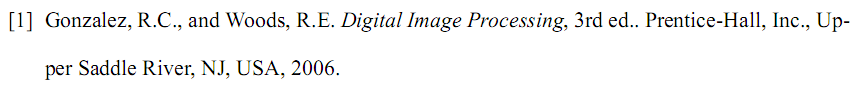
\includegraphics[width=\textwidth]{gonzalez.png}

این شیوهٔ تعریف مراجع بسیار ابتدایی است و اگر فرمت مراجع، ترتیب یا تعداد آنها را خواسته باشید تغییر دهید، به عنوان مثال ابتدا حرف اول نام نویسنده بیاید و سپس نام خانوادگی، باید همه کارها را به صورت دستی انجام دهید!
چون در یک \پ یا مقاله باید کنترل کاملی بر مراجع خود داشته باشید و به راحتی بتوانید قالب مراجع را عوض کنید، بنابراین می‌بایست از \lr{Bib\TeX} استفاده کنید که درپیوست  \ref{app:refMan} به  آن پرداخته خواهد شد.
		% پیوست اول: آشنایی مقدماتی با لاتک
%% !TeX root=../main.tex

\chapter{‌جدول، نمودار و الگوریتم در لاتک}
\label{app:latex:more}
%\thispagestyle{empty}

در این بخش نمونه مثالهایی از جدول، شکل، نمودار، الگوریتم و معادلات ریاضی را در لاتک خواهیم دید.
دقت کنید که در پایان‌نامه‌ها و مقالات، باید قاعدهٔ «ارجاع به جلو%
\LTRfootnote{Forward Referencing}»
رعایت شود؛ یعنی ابتدا در متن به شمارهٔ شکل، جدول یا معادله اشاره شود و بعد از آن (زیر آن) خود شکل، جدول یا معادله رسم شود. (توضیحات بیشتر در قسمت
\ref{sec:floatObjs}).

\section{جدول}
دستور اصلی برای رسم جدول در لاتک 
\verb|tabular|
می‌باشد که جدول
\eqref{tab:motionModels}
با استفاده از آن کشیده شده است؛ در
\verb|tabular|
عرض جدول برابر با مجموع عرض ستون‌ها و حداکثر مساوی عرض متن است.
\begin{table}[ht]
\caption{مدلهای تبدیل.}
\label{tab:motionModels}
\centering
\onehalfspacing
\begin{tabular}{|r|c|l|r|}
	\hline نام مدل & درجه آزادی & تبدیل مختصات & توضیح \\ 
	\hline انتقالی & ۲ & $\begin{aligned} x'=x+t_x \\ y'=y+t_y \end{aligned}$  &  انتقال دوبعدی\\ 
	\hline اقلیدسی & ۳ & $\begin{aligned} x'=x\cos\theta - y\sin\theta+t_x \\ y'=x\sin\theta+y\cos\theta+t_y \end{aligned}$  &  انتقالی+دوران \\ 
	\hline 
\end{tabular} 
\end{table}

برای اینکه عرض جدول قابل کنترل باشد، باید از دستورات
\verb|tabularx|،
\verb|tabulary| یا
\verb|tabu|
استفاده کرد که راهنمای آنها در اینترنت وجود دارد.
مثلاً جدول
\ref{tab:motionModelsCont}
با
\verb|tabularx|
رسم شده که عرض جدول در آن ثابت بوده و ستون‌های از نوع
\verb|X|
عرض خالی جدول را پر می‌کنند.
\begin{table}[ht]
	\caption{مدلهای تبدیل دیگر.}
	\label{tab:motionModelsCont}
	\centering
	\onehalfspacing
	\begin{tabularx}{\textwidth}{|r|c|l|X|}
		\hline نام مدل & درجه آزادی & تبدیل مختصات & توضیح \\ 
		\hline مشابهت & ۴ & $\begin{aligned} x'=sx\cos\theta - sy\sin\theta+t_x \\ y'=sx\sin\theta+sy\cos\theta+t_y  \end{aligned}$  & اقلیدسی+تغییرمقیاس \\ 		
		\hline آفین & ۶ & $\begin{aligned} x'=a_{11}x+a_{12}y+t_x \\ y'=a_{21}x+a_{22}y+t_y \end{aligned}$  & مشابهت+اریب‌شدگی \\
		\hline
	\end{tabularx}
\end{table}

\section{معادلات ریاضی و ماتریس‌ها}
تقریباً هر آنچه دانشجویان برای نوشتن فرمول‌های ریاضی لازم دارند، در کتاب 
\lr{mathmode}
آمده است. کافیست در خط فرمان، دستور زیر را وارد کنید:
\begin{latin}
	\texttt{texdoc mathmode}
\end{latin}
متن زیر شامل انواعی از اشیاء ریاضی است که با ملاحظه کدش می‌توانید با دستورات آن آشنا شوید.\\
شناخته‌شده‌ترین روش تخمین ماتریس هوموگرافی الگوریتم تبدیل خطی مستقیم (\lr{DLT\LTRfootnote{Direct Linear Transform}}) است.  فرض کنید چهار زوج نقطهٔ متناظر در دو تصویر در دست هستند،  $\mathbf{x}_i\leftrightarrow\mathbf{x}'_i$   و تبدیل با رابطهٔ
  $\mathbf{x}'_i = H\mathbf{x}_i$
  نشان داده می‌شود که در آن:
\[\mathbf{x}'_i=(x'_i,y'_i,w'_i)^\top  \]
و
\[ H=\left[
\begin{array}{ccc}
h_1 & h_2 & h_3 \\ 
h_4 & h_5 & h_6 \\ 
h_7 & h_8 & h_9
\end{array} 
\right]\]
رابطه زیر را برای الگوریتم  \eqref{alg:DLT} لازم داریم.
\begin{equation}
\label{eq:DLT_Ah}
\left[
\begin{array}{ccc}
	0^\top & -w'_i\mathbf{x}_i^\top & y'_i\mathbf{x}_i^\top \\ 
	w'_i\mathbf{x}_i & 0^\top & -x'_i\mathbf{x}_i^\top \\ 
	- y'_i\mathbf{x}_i^\top & x'_i\mathbf{x}_i^\top & 0^\top
\end{array} 
\right]
\left(
\begin{array}{c}
	\mathbf{h}^1 \\ 
	\mathbf{h}^2 \\ 
	\mathbf{h}^3
\end{array} 
\right)=0
\end{equation}

\section{الگوریتم}

\subsection{الگوریتم ساده با دستورهای فارسی}
با مفروضات فوق، الگوریتم \lr{DLT} به صورت نشان داده شده در الگوریتم \eqref{alg:DLT}  خواهد بود.
\begin{algorithm}[ht]
\onehalfspacing
\caption{الگوریتم \lr{DLT} برای تخمین ماتریس هوموگرافی.} \label{alg:DLT}
\begin{algorithmic}[1]
\REQUIRE $n\geq4$ زوج نقطهٔ متناظر در دو تصویر 
${\mathbf{x}_i\leftrightarrow\mathbf{x}'_i}$،\\
\ENSURE ماتریس هوموگرافی $H$ به نحوی‌که: 
$\mathbf{x}'_i = H \mathbf{x}_i$.
  \STATE برای هر زوج نقطهٔ متناظر
$\mathbf{x}_i\leftrightarrow\mathbf{x}'_i$ 
ماتریس $\mathbf{A}_i$ را با استفاده از رابطهٔ \ref{eq:DLT_Ah} محاسبه کنید.
  \STATE ماتریس‌های ۹ ستونی  $\mathbf{A}_i$ را در قالب یک ماتریس $\mathbf{A}$ ۹ ستونی ترکیب کنید. 
  \STATE تجزیهٔ مقادیر منفرد \lr{(SVD)}  ماتریس $\mathbf{A}$ را بدست آورید. بردار واحد متناظر با کمترین مقدار منفرد جواب $\mathbf{h}$ خواهد بود.
  \STATE  ماتریس هوموگرافی $H$ با تغییر شکل $\mathbf{h}$ حاصل خواهد شد.
\end{algorithmic}
\end{algorithm}

\subsection{الگوریتم پیچیده و تودرتو با دستورهای فارسی}
الگوریتم \ref{alg:simulation-random}، یک الگوریتم ترکیبی و تودرتو است که با کمک دستورهای بستهٔ \lr{algorithmic} نوشته شده است.

\begin{algorithm}[p]
    \onehalfspacing
    \caption{الگوریتم اجرای برنامهٔ شبیه‌سازی}
    \label{alg:simulation-random}
    \begin{algorithmic}[1]
        \REQUIRE زمان $t_{max}$ به عنوان زمان لازم برای انجام شبیه سازی،\\
        \REQUIRE  گراف شبکه برای شبیه سازی،
        \ENSURE جدول تغییرات گراف از لحظهٔ ۰ تا t.
        \FOR {تمام لحظات در بازهٔ ۰ تا $t_{max}$}
            \FOR {تمام پیوند‌ها}
                \STATE محاسبهٔ ضریب و نرخ انتقال پیوند
                \STATE محاسبهٔ کیفیت و نرخ یادگیری
            \ENDFOR
            \FOR {تمام گره‌ها}
                \STATE محاسبهٔ نرخ انتقال گره
                \STATE محاسبهٔ وضعیت جدید
            \ENDFOR
            \IF {تغییرات از مقدار $\delta$ کمتر است}
                \STATE شکستن حلقه
                \COMMENT{این شرط برای پایان قبل از رسیدن به محدودیت زمانی است، اگر تغییرات کمتر از $\delta$ باشد}
            \ELSIF {زمان اجرای برنامه بیش از حد طول کشیده \AND $t>100$}
                \STATE شکستن حلقه
            \ENDIF
        \ENDFOR
        \PRINT {زمان اجرای برنامه}
        \RETURN {ماتریس تغییرات زمانی}
    \end{algorithmic}
\end{algorithm}

\subsection{الگوریتم با دستورهای لاتین}
الگوریتم \ref{alg:RANSAC} یک الگوریتم با دستورهای لاتین است.

\begin{algorithm}[ht]
\onehalfspacing
\caption{الگوریتم \lr{RANSAC} برای تخمین ماتریس هوموگرافی.} \label{alg:RANSAC}
\begin{latin}
\begin{algorithmic}[1]
\REQUIRE $n\geq4$ putative correspondences, number of estimations, $N$, distance threshold $T_{dist}$.\\
\ENSURE Set of inliers and Homography matrix $H$.
\FOR{$k = 1$ to $N$}
  \STATE Randomly choose 4 correspondence,
  \STATE Check whether these points are colinear, if so, redo the above step
  \STATE Compute the homography $H_{curr}$ by DLT algorithm from the 4 points pairs,
  \STATE $\ldots$ % الگوریتم کامل نیست
  \ENDFOR
  \STATE Refinement: re-estimate H from all the inliers using the DLT algorithm.
\end{algorithmic}
\end{latin}
\end{algorithm}

\section{کد}
درج کد به زبان‌های مختلف به سادگی امکان‌پذیر است. برنامه
\ref{code:matlabEx}
یک قطعه کد
\lr{MATLAB}
را نشان می‌دهد.
\begin{figure}[ht]
	\begin{LTR}
        \singlespacing
		\lstinputlisting[language=MATLAB, caption={نمونه کد \lr{MATLAB}}, label={code:matlabEx}]{MatlabExample.m}
        % \doublespacing
	\end{LTR}
\end{figure}

\section{تصویر}
نمونهٔ یک تصویر را در فصل قبل دیدیم. دو تصویر شیر کنار هم را نیز در شکل
\ref{fig:twoLion}
مشاهده می‌کنید.
\begin{figure}[ht]
\centering 
\subfloat[شیر ۱]{ \label{fig:twolion:one}
\includegraphics[width=0.3\textwidth]{lion}}
%\hspace{2mm}
\subfloat[شیر ۲]{ \label{fig:twolion:two}
\includegraphics[width=0.3\textwidth]{lion}}%
\caption{دو شیر}
\label{fig:twoLion} %% label for entire figure
\end{figure}

\section{نمودار}
لاتک بسته‌هایی با قابلیت‌های زیاد برای رسم انواع مختلف نمودارها دارد. مانند بسته‌های \lr{Tikz} و  \lr{PSTricks}. توضیح اینها فراتر از این پیوست کوچک است.%
\footnote{
مثال‌هایی از بکارگیری بسته
\lr{Tikz}
را می‌توانید در
\url{http://www.texample.net/tikz/examples/}
ببینید. توصیه می‌شود دانشجویانی که قصد درج اشکالی مانند گراف را در سند خود دارند، مثالهایی از سایت مذکور را ملاحظه فرمایند.
}
یک نمودار رسم شده با بستهٔ 
\lr{TikZ}
 در شکل 
\ref{fig:parabola}
نشان داده شده است.
\begin{figure}[t]
\centering
\begin{tikzpicture}[scale=2.5]
  \shade[top color=blue,bottom color=gray!50] 
      (0,0) parabola (1.5,2.25) |- (0,0);
  \draw (1.05cm,2pt) node[above] 
      {$\displaystyle\int_0^{3/2} \!\!x^2\mathrm{d}x$};

  \draw[style=help lines] (0,0) grid (3.9,3.9)
       [step=0.25cm]      (1,2) grid +(1,1);

  \draw[->] (-0.2,0) -- (4,0) node[right] {$x$};
  \draw[->] (0,-0.2) -- (0,4) node[above] {$f(x)$};

  \foreach \x/\xtext in {1/1, 1.5/1\frac{1}{2}, 2/2, 3/3}
    \draw[shift={(\x,0)}] (0pt,2pt) -- (0pt,-2pt) node[below] {$\xtext$};

  \foreach \y/\ytext in {1/1, 2/2, 2.25/2\frac{1}{4}, 3/3}
    \draw[shift={(0,\y)}] (2pt,0pt) -- (-2pt,0pt) node[left] {$\ytext$};

  \draw (-.5,.25) parabola bend (0,0) (2,4) node[below right] {$x^2$};
\end{tikzpicture}
\caption{یک نمودار زیبا با ارقام فارسی و قابلیت بزرگ‌نمایی بسیار، بدون از دست دادن کیفیت.}
\label{fig:parabola}
\end{figure}

\section{نحوه قرارگیری اشیای شناور}
\label{sec:floatObjs}
شکل‌ها، جداول و الگوریتم‌ها در لاتک اشیای شناور محسوب می‌شوند؛ یعنی خود لاتک تصمیم می‌گیرد آنها را در کجای صفحه ترسیم کند تا زیباتر باشد. اما می‌توان به لاتک توصیه کرد که آن را در قسمت خاصی از صفحه رسم کند. برای اینکه قاعدهٔ «ارجاع به جلو» رعایت شود باید فقط از پرچم
\verb|[ht]|
استفاده کرد، که می‌گوید اگر جا شد شکل را دقیقاً در همین مکان و در غیراینصورت در بالای صفحه بعد رسم کن.
بنابراین دستورات درج تصویر، جدول و الگوریتم به صورت زیر باید باشند:

\begin{latin}
\begin{verbatim}
	\begin{figure/table/algorithm}[ht]
		...
	\end{figure/table/algorithm}
\end{verbatim}
\end{latin}
		% پیوست دوم: جدول، نمودار و الگوریتم در لاتک
%% !TeX root=../main.tex
\chapter{مراجع، واژه‌نامه و حاشیه‌نویسی}
\label{app:refMan}
%\thispagestyle{empty}

\section{مراجع و نقل‌قول‌ها}
\label{sec:refUsage}
منابعِ پایان‌نامه، پایه و اساس تحقیق شما به حساب می‌آیند و ضرورت انجام مطالعه و روش‌های به کار رفته در بسیاری از قسمت‌های آن، به کمک منابع صورت می‌گیرد. در استفاده از مراجع علمی در پایان‌نامه، باید سعی کنید بیشتر از
\textbf{منابع چاپ‌شده و مهم}
استفاده کنید و
\emph{ارجاع به داده‌های چاپ نشده، خلاصه‌ها و پایان‌نامه‌ها، سبب به‌هم‌خوردگی و کاهش اعتبار قسمت ارجاع منابع می‌شود.}
استفاده از منابع و نقل قول‌هایی به تحقیق شما ارزش می‌دهند که
\textbf{در راستای هدف تحقیق بوده و به آن اعتبار ببخشند.}
برخی از دانش‌جویان تصوّر می‌کنند که کثرت نقل‌قول‌ها و ارجاعات زیاد، مهم‌ترین معیار علمی شدن پایان‌نامه است؛ حال آنکه استناد به تعداد کثیری از منابع بدون مطالعه دقیق آنها و استفادهٔ مستقیم در پایان‌نامه، می‌تواند نشان‌دهندهٔ عدم احساس امنیت نویسنده باشد!

دو روش برای استفاده از نتایج، جملات، داده‌ها و روش‌های دیگران وجود دارد. یکی نقل‌قول مستقیم و دقیق است و دیگری استفاده غیرمستقیم در متن مقاله، که در ادامه به قواعد این دو نوع نقل‌قول و ارجاع‌دهی اشاره می‌کنیم:
\begin{description}
	\item[نقل‌قول مستقیم:]
	نقل‌قول مستقیم باید دقیق و بدون هیچ تغییری در جملات باشد. بهتر است این‌گونه نقل‌قول‌ها تا حد امکان کوتاه باشد. جملات کوتاه داخل گیومه قرار می‌گیرند و باید به منبع دقیق آن، طبق روش ارجاع‌دهی به منابع، اشاره شود. به عنوان مثال در
	\cite{persianbib87userguide}
	آمده است که:
	\begin{quote}
		«با استفاده از فیلد
		\lr{AUTHORFA}
		می‌توان معادل فارسی نام نویسندگان مقالات لاتین را در متن داشت. معمولاً در اسناد فارسی خواسته می‌شود که پس از ذکر معادل فارسی نام نویسنده، نام لاتین نویسنده(ها) به عنوان پاورقی درج شود
		\citep{persianbib87userguide}.»
	\end{quote}
	\item[نقل‌قول غیرمستقیم:]
	نقل‌قول غیرمستقیم به معنی استفاده از ایده‌ها، نتایج، روش‌ها و داده‌های دیگران در درون متنِ پایان‌نامه، ولی به سبک خودتان و متناسب و هماهنگ با روند پایان‌نامهٔ شماست. در این حالت نیز باید متناسب با شیوهٔ ارجاع‌دهی به آن استناد شود.
\end{description}

با توجه به وجود سبک‌های مختلف ارجاع‌دهی، باید
\textbf{روش قابل قبول و یکسانی}
در طول پایان‌نامه برای اشاره به مراجع در متن و همچنین تهیه فهرست مراجع در انتهای پایان‌نامه بکار رود. مثلاً برای پایان‌نامه‌های مهندسی می‌توان از سبک ارجاع‌دهی
\lr{IEEE}%
\LTRfootnote{\url{http://www.ieee.org/documents/ieeecitationref.pdf}}
یا
\lr{acm}
استفاده کرد. طبیعتاً باید تناظر یک‌به‌یک بین فهرست مراجع در انتهای گزارش و مراجع مورد استفاده در متن باشد%
\footnote{البته گاهی ممکن است محقق مرجعی را مورد مطالعه قرار داده لیکن در متن به آن اشاره نکرده باشد؛ برخی معتقدند در این موارد نیز آوردن آن در فهرست مراجع، اشکالی ندارد، به این شرط که از عنوان «فهرست منابع» به جای «فهرست مراجع» استفاده شود.}.

برای سهولت مدیریت مراجعِ \پ%
، اکیداً توصیه می‌شود از یک ابزار «مدیریت منابع» (با خروجی
\texorpdfstring{\lr{Bib\TeX}}{Bib\TeX}%
) همچون
\lr{Mendeley}،
\lr{Zotero},
\lr{EndNote}
یا
\lr{Citavi}
استفاده کنید.

\subsection{ مدیریت مراجع با  \texorpdfstring{\lr{Bib\TeX}}{Bib\TeX}}
در بخش \ref{Sec:Ref} اشاره شد که با دستور 
 \lr{\textbackslash bibitem}
  می‌توان یک مرجع را تعریف نمود و با فرمان
 \lr{\textbackslash cite}
  به آن ارجاع داد. این روش برای تعداد مراجع زیاد و تغییرات آنها مناسب نیست. برای مدیریت منابع زیاد، سه بستهٔ
\lr{BibTeX} (پیش‌فرض),
\lr{natbib}
(ارجاع‌دهی در متن به صورت نویسنده-سال)
و \lr{BibLaTeX} (جدید و منعطف‌پذیر)
وجود دارند. در ادامه توضیحاتی در مورد مدیریت منابع با \lr{BibTeX} و \lr{natbib} در زی‌پرشین خواهیم آورد که همراه با توزیع‌های معروف تِک عرضه می‌شوند
\footnote{روش \lr{BibLaTeX} هنوز برای متون فارسی به درستی ترجمه نشده است.}.

یکی از روش‌های قدرتمند و انعطاف‌پذیر برای نوشتن مراجعِ مقالات و مدیریت مراجع در لاتک، استفاده از  \lr{BibTeX} است.
 روش کار با بیب‌تک به این صورت است که مجموعهٔ همهٔ مراجعی را که در \پ استفاده کرده یا خواهیم کرد، 
در پروندهٔ جداگانه‌ای با پسوند
\lr{bib}
نوشته و به آن فایل در سند خودمان به صورت مناسب لینک می‌دهیم.
 کنفرانس‌ها یا مجله‌های گوناگون برای نوشتن مراجع، قالب‌ها یا قراردادهای متفاوتی دارند که به آنها استیل‌های مراجع گفته می‌شود.
 در این حالت به کمک ‌استیل‌های بیب‌تک خواهید توانست تنها با تغییر یک پارامتر در پروندهٔ ورودی خود، مراجع را مطابق قالب موردنظر تنظیم کنید. 
 بیشتر مجلات و کنفرانس‌های معتبر یک فایل سبک
 (\lr{BibTeX Style})
با پسوند \lr{bst} در وب‌گاه خود می‌گذارند که برای همین منظور طراحی شده است.

به جز نوشتن مقالات، این سبک‌ها کمک بسیار خوبی برای تهیهٔ مستندات علمی همچون پایان‌نامه‌هاست که فرد می‌تواند هر قسمت از کارش را که نوشت مراجع مربوطه را به بانک مراجع خود اضافه نماید. با داشتن چنین بانکی از مراجع، وی خواهد توانست به راحتی یک یا چند ارجاع به مراجع و یا یک یا چند بخش را حذف یا اضافه ‌نماید؛ 
مراجع به صورت خودکار مرتب شده و
\textbf{فقط مراجع ارجاع داده شده در قسمت کتاب‌نامه خواهندآمد.}
قالب مراجع به صورت یکدست مطابق سبک داده شده بوده و نیازی نیست که کاربر درگیر قالب‌دهی به مراجع باشد. 

\subsection{سبک‌های مورد تأیید دانشگاه تهران}
طبق «دستورالعمل نگارش و تدوین پایان‌نامه» دانشگاه تهران در
\cite{UTThesisGuide}،
ارجاع در متن می‌تواند مطابق با هر یک از دو الگوی هاروارد یا ونکوور باشد:
\singlespacing
\begin{description}
	\item[سیستم نویسنده-سال (هاروارد):]
	ذکر نام نویسنده و سال نشر در متن. در این الگو مراجع بر اساس حروف الفبا تنظیم می‌گردند.
	\item[سیستم شماره‌دار (ونکوور):]
	ارجاع به مراجع به کمک شماره در متن. در این الگو شماره هر مرجع به ترتیب ظاهر شدن آن در متن در داخل کروشه قرار می‌گیرد. فهرست مراجع نیز بر اساس شماره مرجع (نه حروف الفبا) تنظیم می‌گردد.
\end{description}
\doublespacing

در مدیریت منابع با
\lr{\textbf{BibTeX}}،
ارجاع‌ها در متن تنها به شکل
\textbf{شماره‌دار (ونکوور)}
امکان‌پذیر است، گرچه فهرست مراجع می‌تواند با روش‌های مختلف مرتب شود. اگر بخواهیم ارجاع‌ها در متن به صورت
\textbf{نویسنده-سال (هاروارد)}
باشد باید از بستهٔ
\lr{\textbf{natbib}}\LTRfootnote{Natural Sciences Citations \& References}
و استیل‌های مختلف آن استفاده کنیم.

هنگام استفاده از روش نویسنده-سال نوع پرانتزگذاری‌ها در وسط و انتهای جمله با هم فرق خواهد داشت. به مثال زیر مطابق با دستورالعمل
\cite{UTThesisGuide}
توجه کنید:

\textit{
ابتدا
\cite{Khalighi87xepersian}
بستهٔ زی‌پرشین را برای حروف‌چینی فارسی اختراع کرد. بعدها سبک‌های ارجاع‌دهی فارسی و قالب‌های پایان‌نامه نیز مبتنی بر آن ساخته شد
\citep{persianbib87userguide}.
ارجاع‌دهی به مراجع لاتین نیز در زی‌پرشین امکان‌پذیر است. مثلاً
\citelatin{Gonzalez02book}
یک کتاب انگلیسی است و به راحتی به مقالات انگلیسی نیز می‌توان ارجاع داد
\citeplatin{kim2016integrated}.}

در این مثال، ۴ ارجاع در وسط و انتهای جمله به مراجع فارسی و انگلیسی آمده است. وقتی از سیستم نویسنده-سال استفاده می‌کنید، بهتر است ارجاع‌های آخر جمله کلاً داخل پرانتر بیاید؛ بدین منظور باید به جای
\verb|\cite|
از
\verb|\citep|
استفاده کنید. اما در سیستم شماره‌دار چون تمام ارجاع‌ها داخل کروشه می‌آیند این امر اهمیت ندارد.\\
نمی‌توانید در متن فارسی، اسم لاتین محقق خارجی را بیاورید و برای جلوگیری از ایجاد ابهام، صرف‌نظر از نام لاتین هم مجاز نیست! توصیه می‌شود که نام محقق خارجی در متن با حروف فارسی و در پاورقی اسم تمام نویسندگان به صورت انگلیسی آورده شود. نحوهٔ رعایت این نکته را می‌توانید در کد مثال بالا ببینید.

گرچه در تمپلت ورد
\cite{UTThesisGuide}،
به صراحت ذکر شده که بهتر است برای پایان‌نامه‌های مهندسی از سبک 
\lr{IEEE}
استفاده شود (که از سیستم ونکوور تبعیت می‌کند)، اما ترتیب فهرست مراجع در
\lr{IEEE}
بر اساس ترتیب ارجاع در متن بوده و
\emph{مراجع انگلیسی و فارسی از هم تفکیک نمی‌شوند}
که متضاد با دستورالعمل
\cite{UTThesisGuide}
و نیز متضاد عرف اکثر پایان‌نامه‌های فارسی است.
بنابراین دقیقاً نمی‌توان سبک خاصی را برای مراجع پایان‌نامه‌های دانشگاه تهران اجبار کرد. مهم این است که
\textbf{سبک ارجاع‌دهی در تمام طول یک کتابچه}
(مثلاً پایان‌نامه، مقالات یک مجله یا کل یک کتاب) یکسان باشد. بهتر است
\textbf{بسته به حوزه پایان‌نامه}،
در این مورد با استاد راهنمای خود مشورت کنید.

\subsection{سبک‌های فارسی قابل استفاده در زی‌پرشین}
تعدادی از سبک‌های فارسی بسته
\lr{Persian-bib}%
\footnote{ برای اطلاع بیشتر به راهنمای بستهٔ
\lr{Persian-bib}
مراجعه فرمایید.}
که برای  زی‌پرشین آماده شده‌اند، عبارتند از:

\singlespacing
\begin{itemize}
\item \emph{سبک‌های شماره‌دار}:
	\begin{description}
	\item [unsrt-fa.bst] این سبک متناظر با \lr{unsrt.bst} می‌باشد. مراجع به ترتیب ارجاع در متن ظاهر می‌شوند.
	\item [plain-fa.bst] این سبک متناظر با \lr{plain.bst} می‌باشد. مراجع بر اساس نام‌خانوادگی نویسندگان، به ترتیب صعودی مرتب می‌شوند.
	 همچنین ابتدا مراجع فارسی و سپس مراجع انگلیسی خواهند آمد.
	\item [acm-fa.bst] این سبک متناظر با \lr{acm.bst} می‌باشد. شبیه \lr{plain-fa.bst} است.  قالب مراجع کمی متفاوت است. اسامی نویسندگان انگلیسی با حروف بزرگ انگلیسی نمایش داده می‌شوند. (مراجع مرتب می‌شوند)
	\item [ieeetr-fa.bst] این سبک متناظر با \lr{ieeetr.bst} می‌باشد. (مراجع مرتب نمی‌شوند)
	\end{description}
	
\item \emph{سبک‌های نویسنده-سال}:
	\begin{description}
	\item [plainnat-fa.bst] این سبک متناظر با \lr{plainnat.bst} می‌باشد. نیاز به بستهٔ \lr{natbib} دارد. (مراجع مرتب می‌شوند)
	\item [chicago-fa.bst] این سبک متناظر با \lr{chicago.bst} می‌باشد. نیاز به بستهٔ \lr{natbib} دارد. (مراجع مرتب می‌شوند)
	\item [asa-fa.bst] این سبک متناظر با \lr{asa.bst} می‌باشد. نیاز به بستهٔ \lr{natbib} دارد. (مراجع مرتب می‌شوند)
	\end{description}
\end{itemize}
\doublespacing

با استفاده از استیل‌های فوق می‌توانید به انواع مختلفی از مراجع فارسی و لاتین ارجاع دهید.
به عنوان مثال‌هایی از
\textbf{مراجع انگلیسی}،
مرجع
\cite{Baker02limits}\footnote{چون فیلد \lr{authorfa} برای این مرجع تعریف نشده در سبک نویسنده-سال با حروف لاتین به آن در متن ارجاع می‌شود که غلط است.}
مقالهٔ یک ژورنال، مرجع
\cite{Amintoosi09video}
مقالهٔ یک کنفرانس، مرجع
\citelatin{Gonzalez02book}
یک کتاب، مرجع
\cite{Khalighi07MscThesis}
پایان‌نامهٔ کارشناسی ارشد و مرجع
\citelatin{Borman04thesis}
یک رسالهٔ دکتری می‌باشد.\\
همچنین در میان
\textbf{مراجع فارسی},
مرجع
\cite{Vahedi87}
مقالهٔ یک مجله، مرجع
\cite{Amintoosi87afzayesh}
مقالهٔ یک کنفرانس، مرجع
\cite{Pedram80osool}
یک کتاب ترجمه‌شده با ذکر مترجمان و ویراستاران، مرجع
\cite{Pourmousa88mscThesis}
پایان‌نامهٔ کارشناسی ارشد%
\footnote{همان‌طور که در بخش
\ref{sec:refUsage}
اشاره شد، بهتر است زیاد از پایان‌نامه‌ها در مراجع استفاده نکنید.}،
مرجع
\cite{Omidali82phdThesis}
یک رسالهٔ دکتری و مراجع
\cite{persianbib87userguide, Khalighi87xepersian}
نمونه‌های متفرقه هستند.

\subsection{ساختار فایل مراجع}
برای استفاده از بیب‌تک باید مراجع خود را در یک فایل با پسوند \lr{bib} ذخیره نمایید. یک فایل \lr{bib} در واقع یک پایگاه داده از مراجع%
\LTRfootnote{Bibliography Database}
شماست که هر مرجع در آن به عنوان یک رکورد از این پایگاه داده
با قالبی خاص ذخیره می‌شود. به هر رکورد یک مدخل%
\LTRfootnote{Entry}
گفته می‌شود. یک نمونه مدخل برای معرفی کتاب \lr{Digital Image Processing} در ادامه آمده است:

\singlespacing
\begin{LTR}
\begin{verbatim}
@BOOK{Gonzalez02image,
  AUTHOR     = {Gonzalez,, Rafael C. and Woods,, Richard E.},
  TITLE      = {Digital Image Processing},
  PUBLISHER  = {Prentice-Hall, Inc.},
  YEAR       = {2006},
  ISBN       = {013168728X},
  EDITION    = {3rd},
  ADDRESS    = {Upper Saddle River, NJ, USA}
}
\end{verbatim}
\end{LTR}
\doublespacing

در مثال فوق، \lr{@BOOK} مشخصهٔ شروع یک مدخل مربوط به یک کتاب و \lr{Gonzalez02book} برچسبی است که به این مرجع منتسب شده است.
 این برچسب بایستی یکتا باشد. برای آنکه بتوان
\textbf{برچسب مراجع}
 را به راحتی به خاطر سپرد و حتی‌الامکان برچسب‌ها متفاوت با هم باشند، معمولاً از قوانین خاصی به این منظور استفاده می‌شود. یک قانون می‌تواند
\textbf{فامیل نویسنده اول + دورقم سال نشر + اولین کلمهٔ عنوان اثر}
باشد. به
\lr{AUTHOR}، \lr{TITLE}، $\dots$ و \lr{ADDRESS}
فیلدهای این مدخل گفته می‌شود، که هر یک با مقادیر مربوط به مرجع پر شده‌اند. ترتیب فیلدها مهم نیست. 

انواع متنوعی از مدخل‌ها برای اقسام مختلف مراجع همچون کتاب، مقالهٔ کنفرانس و مقالهٔ ژورنال وجود دارد که برخی فیلدهای آنها با هم متفاوت است. 
نام فیلدها بیانگر نوع اطلاعات آن می‌باشد. مثالهای ذکر شده در فایل \lr{MyReferences.bib} کمک خوبی برای شما خواهد بود. 
%این فایل یک فایل متنی بوده و با ویرایشگرهای معمول همچون \lr{Notepad++} قابل ویرایش می‌باشد. برنامه‌هایی همچون 
%\lr{TeXMaker}
% امکاناتی برای نوشتن این مدخل‌ها دارند و به صورت خودکار فیلدهای مربوطه را در فایل \lr{bib}  شما قرار می‌دهند.  
با استفاده از سبک‌های فارسی آماده شده، محتویات هر فیلد می‌تواند به فارسی نوشته شود؛ ترتیب مراجع و نحوهٔ چینش فیلدهای هر مرجع را سبک مورد استفاده  مشخص خواهد کرد.

\textbf{در فایل 
\lr{MyReferences.bib}
 که همراه با این \پ هست، مثال‌های مختلفی از مراجع آمده‌اند که برای درج مراجع خود، تنها کافیست مراجع‌تان را جایگزین موارد مندرج در آن نمایید.
}

برای بسیاری از مقالات لاتین حتی لازم نیست که مدخل مربوط به آنرا خودتان بنویسید. با جستجوی 
\textbf{نام مقاله + کلمه
\lr{bibtex}}
در اینترنت سایت‌های بسیاری همچون
\lr{ACM} و \lr{ScienceDirect}
را خواهید یافت که مدخل
\lr{bibtex}
مربوط به مقاله شما را دارند و کافیست آنرا به انتهای فایل
\lr{MyReferences.bib}
اضافه کنید.

\subsection{نحوه اجرای \texorpdfstring{\lr{Bib\TeX}}{Bib\TeX}}
پس از قرار دادن مراجع خود، برای ساخت فایل خروجی می‌توانید دستور زیر را (در ترمینال یا از طریق \lr{Texmaker}) اجرا کنید:%
\footnote{فایل \lr{latexmkrc} باید در کنار \lr{main.tex} وجود داشته باشد.}

\singlespacing
\begin{LTR}
	\begin{verbatim}
		latexmk -bibtex -pdf main.tex
	\end{verbatim}
\end{LTR}
\doublespacing
ابزار \lr{latexmk} مراحل مختلف ساخت خروجی لاتک را به طور خودکار و بهینه انجام می‌دهد و هر بار فقط مراحلی را که لازم باشد تکرار می‌کند.
روش دستی‌تر این است که یک بار \lr{XeLaTeX} را روی سند خود اجرا نمایید، سپس \lr{bibtex} و پس از آن هم ۲ بار \lr{XeLaTeX} را. در \lr{TeXMaker} کلید \lr{F11} و در \lr{TeXWorks} هم گزینهٔ \lr{BibTeX} از منوی \lr{Typeset}، \lr{BibTeX} را روی سند شما اجرا می‌کنند.

\section{واژه‌نامه‌ها و فهرست اختصارات}
\gls{Gloss}
یا فرهنگ لغات، مجموعه‌ای از اصطلاحات و تعاریف خاص و فنی است که معمولاً در انتهای یک کتاب می‌آید. چون پایان‌نامه خود یک متن تخصصی بلند محسوب می‌شود، استفاده از فرهنگ لغات در انتهای آن به شدت توصیه می‌شود، خصوصاً که احتمال استفاده از لغات تخصصی لاتین در آن بالاست.
واژه‌نامه‌هایی که در انتهای کتاب‌های انگلیسی می‌آیند معمولاً تک‌زبانه هستند و معنی یک اصطلاح تخصصی در آنها، عمدتاً به صورت یک
\gls{Description}
طولانی آورده می‌شود. اما چون در متون فارسی، آوردن لغات انگلیسی مجاز نیست و باید معادل فارسی آنها وارد شود، جهت رفع ابهام معمولاً واژه‌نامهٔ فارسی به انگلیسی (و برعکس) در انتهای کتاب درج شده و  
\glspl{Description}
در صورت نیاز در متن آورده می‌شوند.

فهرست
\glspl{Acronym}
شامل نمادهای کوتاهی است که اغلب از حروف ابتدایی کلمات یک عبارت طولانی ساخته شده‌اند. با اینکه
\glspl{Acronym}
با حروف (بزرگ) لاتین نوشته می‌شوند، اما چون کوتاهند استفاده از آنها در میان متن فارسی مجاز است. با این حال برای رفع ابهام، عرف است که فهرستی از آنها شامل معنی هر نماد، در کنار دیگر فهرست‌ها در ابتدای متن درج شود.

در این قالب پایان‌نامه، برای ساخت و مدیریت واژه‌نامه و فهرست اختصارات از بستهٔ پیشرفتهٔ
\lr{glossaries}
با موتور واژه‌نامه‌سازی
\lr{xindy}
استفاده می‌شود. تنظیمات بهینهٔ این بسته در فایل
\lr{glossaries-settings.tex}
عبارتند از:
\begin{itemize}
	\item
قبل از درج واژه‌ها در متن، باید مدخل آنها با دستور زیر (ترجیحاً در فایل جدای \lr{words.tex}) تعریف شود:
	\begin{LTR}
	\verb|\newword{Label}{Word}|\{واژه\}\{واژه‌ها\}
	\end{LTR}
	
	\item
قبل از وارد کردن علائم اختصاری در متن، باید مدخل آنها نیز (ترجیحاً در فایل \lr{acronyms.tex}) به صورت زیر تعریف شود:
	\begin{LTR}
	\verb|\newacronym{Label}{Acr}|\{معنی‌اختصار\}
	\end{LTR}

	\item
جهت درج یک علامت اختصاری یا معادل یک واژه تخصصی، کافی است از دستور
	\verb|gls{Label}|
در متن استفاده کنید. دستور
	\verb|glspl{Label}|
نیز برای آوردن معادل یک لغت در حالت جمع ساخته شده است.
	
	\item
هنگام اولین استفاده از یک معادل فارسی یا اختصار در متن، معادل انگلیسی یا معنی آن در پاورقی آورده می‌شود. در صورتی که هر یک از این پیش‌فرض‌ها را دوست ندارید با ویرایش فایل
	\lr{glossaries-settings.tex}
می‌توانید آن را تغییر دهید.

	\item
در انتهای پایان‌نامه با دستور
\verb|\printglossary|
فهرست کلمات استفاده‌شده به ترتیب الفبای فارسی (واژه‌نامه فارسی به انگلیسی) و الفبای انگلیسی (واژه‌نامه انگلیسی به فارسی) درج می‌شود.
\end{itemize}

به عنوان مثال، با مشاهدهٔ کد این نوشته، نحوهٔ درج معادل فارسی
\gls{RandomVariable}
را در متن مشاهده می‌کنید.
در نمایش واژهٔ
\gls{RandomVariable}
برای بار دوم، معادل لاتین در پاورقی نمی‌آید.
در مورد درج علائم اختصاری، مثلاً می‌توان به رابطهٔ
\gls{F}
اشاره کرد.

\section{حاشیه‌نویسی در نسخه پیش‌نویس}
اصلاح و بازبینی چندین و چندبارهٔ یک پایان‌نامه یا مقاله، از معمول‌ترین امور در نگارش آن می‌باشد. فرض کنید دانشجو پایان‌نامه یا مقالهٔ خود را (کامل یا ناقص) نوشته و می‌خواهد نظر استاد راهنما، اعضای آزمایشگاه یا دیگر متخصصین را در مورد آن جویا شود. به جز مشاورهٔ حضوری، تلفنی یا از طریق ایمیل، برای اظهارنظر دقیق بر نوشته، می‌توان از ابزارهای حاشیه‌نویسی در فایل
\lr{PDF}
یا \lr{tex}
نیز استفاده کرد.

یک راهکار مناسب برای حاشیه‌نویسی در فایل \lr{tex}، استفاده از بسته 
\lr{todonotes}
می‌باشد که آقای خلیقی به تازگی امکان استفاده از آن را برای فارسی‌زبانان نیز فراهم آورده‌اند.
بدین منظور، هر جایی که خواستید نکته یا نکاتی را در حاشیه متن یادداشت کنید، کافی است دستور زیر را وارد نمایید:
\begin{latin}
\verb|\todo{NOTE}|
\end{latin}
مثلاً استاد راهنما می‌تواند از دانشجو بخواهد که در بخشی توضیح بیشتری دهد.
\todo{
توضیح بیشتری لازم است.
}
استاد راهنما یا داور حتی می‌تواند محل پیشنهادی برای درج یک تصویر را نیز به راحتی برای دانشجو مشخص کند.
\missingfigure[figwidth=\textwidth,figcolor=white]{یک تصویر از خروجی الگوریتم 
\ref{alg:RANSAC}
را در اینجا قرار دهید.}
یکی دیگر از امکانات این بسته آن است که می‌توان فهرست نکات را در ابتدای سند داشت. بسته 
\lr{todonotes}
امکانات بسیاری دارد
\todo[fancyline,color=green!30]{مرجع این مطلب؟}
که در راهنمای آن معرفی شده است و با اجرای دستور زیر در خط فرمان می‌توانید آنها را مشاهده کنید:
\begin{latin}	
	\texttt{texdoc todonotes}
\end{latin}	
دقت کنید که توضیحات حاشیه‌ای و فهرست کارهای باقیمانده (نکات)،
\textbf{فقط در نسخه
\gls{Draft}}
قابل دیدن هستند و در نسخه نهایی، نمایش داده نخواهند شد.
برای استفاده از حالت
\gls{Draft}
باید گزینه 
\lr{draft}
به دستور 
\verb|\documentclass|
در ابتدای فایل 
\lr{main.tex}
اضافه شود.
هنگامی‌که سند شما در حالت 
\gls{Draft}
باشد:

\singlespacing
\begin{enumerate}
\item 
هیچ یک از صفحات آغازین پایان‌نامه، تا فهرست مطالب نمایش داده نمی‌شود (به جز صفحه اول).
\item
روی صفحه اول عبارت «پیش‌نویس» به صورت درشت و کم‌رنگ نمایش داده می‌شود.
\item
فهرست نکات درج شده توسط
\lr{todo}،
پس از فهرست اصلی و با عنوان «فهرست کارهای باقیمانده» نمایش داده می‌شود.
\item
شماره صفحاتی که به هر مرجع ارجاع داده شده است در بخش مراجع نمایش داده می‌شود
\footnote{اعمال گزینهٔ
\lr{pagebackref}
برای بستهٔ
\lr{hyperref}.
}.
\end{enumerate}
\doublespacing
هر یک از موارد بالا تا زمانی که نسخه نهایی \پ نیاز نباشد بسیار مورد توجه و مفید واقع می‌شوند.
   	% پیوست سوم: مراجع، واژه‌نامه و حاشیه‌نویسی

% برگرداندن شماره‌بندی صفحات فصول
 \let\chapter\Chapter
\pagenumbering{tartibi} % اول، دوم، ...
%\baselineskip=.75cm

% چاپ واژه‌نامه‌ها و نمایه 
\onehalfspacing
\printglossary
\printindex

\begin{latin}
\baselineskip=.6cm
\latinabstract
\latinTitlePage
\end{latin}
\label{LastPage}

\end{document}
